\documentclass{llncs}
\usepackage[letterpaper,margin=1in]{geometry}
\usepackage{amsmath,amssymb}
\usepackage{booktabs}
\usepackage{array}
\usepackage{graphicx}
\usepackage{pgfplots}
\usepgfplotslibrary{groupplots}
\usetikzlibrary{arrows.meta,positioning,calc}
\pgfplotsset{compat=1.18}
\usepackage[protrusion=false]{microtype}
\usepackage[numbers,sort&compress]{natbib}
\usepackage{placeins}
\usepackage{float}
\usepackage[T1]{fontenc}
\usepackage{lmodern}
\usepackage[hidelinks,hypertexnames=false]{hyperref}
\let\small\normalsize
\let\footnotesize\normalsize
\setlength{\tabcolsep}{6pt}
\makeatletter
\setlength{\@fptop}{0pt}
\setlength{\@fpsep}{12pt}
\makeatother
\renewcommand{\refname}{References}
\renewcommand{\bibsection}{\section*{\refname}\thispagestyle{plain}}
\renewcommand{\topfraction}{0.95}
\renewcommand{\bottomfraction}{0.85}
\renewcommand{\textfraction}{0.05}
\renewcommand{\floatpagefraction}{0.75}
\setcounter{topnumber}{3}
\setcounter{bottomnumber}{2}
\setcounter{totalnumber}{4}
\clubpenalty=10000
\widowpenalty=10000
\displaywidowpenalty=10000
\emergencystretch=1em
\title{\texorpdfstring{SCEPI: Single-Mutant-Conditioned Epistasis Prediction\\for Compensatory Protein Variant Discovery}{SCEPI: Single-Mutant-Conditioned Epistasis Prediction for Compensatory Protein Variant Discovery}}
\titlerunning{SCEPI for compensatory protein variant discovery}
\author{Dong Xu\inst{1,2,4} \and Jiayu Zhang\inst{2} \and Zhangfan Yang\inst{3} \and Jun Zhang\inst{1,4} \and Zexuan Zhu\inst{1,4} \and Junkai Ji\inst{1,2,4}\thanks{Corresponding author.}}
\authorrunning{Dong Xu et al.}
\institute{School of Artificial Intelligence, Shenzhen University, 518060 Shenzhen, China
\and EasternDawn, Shenzhen, China
\and School of Computer Science, University of Nottingham Ningbo, 315100 Ningbo, China
\and Intelligent Computing Center, Shenzhen University, 518060 Shenzhen, China}
\hypersetup{pdftitle={SCEPI: Single-Mutant-Conditioned Epistasis Prediction for Compensatory Protein Variant Discovery},pdfauthor={Dong Xu, Jiayu Zhang, Zhangfan Yang, Jun Zhang, Zexuan Zhu, Junkai Ji}}

\begin{document}
\maketitle
\pagestyle{plain}
\thispagestyle{plain}
\raggedbottom

\begin{abstract}
We introduce Single-mutant-Conditioned Epistasis Prediction (SCEPI) for discovering compensatory double mutants from individually damaging substitutions. A shared cross-protein interaction function receives measured single-mutant effects alongside protein representations. The same measurements calibrate individual effects outside the interaction network. Training uses source combination measurements and withholds target double-mutant labels. Across 155 held-out proteins, SCEPI achieves mean residual root mean squared error of 0.590 kcal/mol, compared with 0.805 for ThermoMPNN-D, 0.847 for Kermut, and 0.853 for calibrated StabilityArc. Selecting ten candidates per protein yields a compensation hit rate of 11.22\% across 120 proteins, compared with 7.07\%, 5.40\%, and 8.75\%, respectively. This is 4.27 times the 2.63\% expectation of uniform random selection from the same candidates. Matched controls separate numerical inputs from availability indicators while retaining external calibration. Measured values supply the main residual-prediction gain. Selection gains persist with the same measured single-effect sum, stricter homology grouping, and measurement-boundary analysis. Existing single-mutant measurements thus guide compensatory discovery in unseen proteins through a transferable interaction model.
\end{abstract}

\section{Introduction}

Compensatory substitutions recover stability or function lost through other sequence changes \citep{davis2009,gong2013,azbukina2022}. Discovering them requires selecting useful combinations of individually damaging substitutions. Single-mutant measurements provide target-specific information for spending a fixed experimental budget on these combinations.

Complete wild-type, single-mutant, and double-mutant measurements define observed nonadditivity \citep{tsuboyama2023}. This contrast includes global phenotype nonlinearity and pair-dependent effects \citep{otwinowski2018,tareen2022}. Measurements from source proteins can supervise a shared interaction function for predicting unmeasured target combinations. Transferable combination predictors already learn from structure or sequence representations \citep{dieckhaus2025,ouyang2023,feller2026}, and target-specific regression uses measured variants \citep{groth2024}. We ask whether target single-mutant measurements add predictive value when supplied directly to the shared interaction function.

SCEPI uses measured single effects in two places. They calibrate individual effects and condition a shared interaction function together with their observation indicators. Within this function, the measured inputs accompany reference and single-mutant representations. Subtraction around a double-mutant cycle cancels endpoint-only offsets and enforces zero interaction at either wild-type endpoint. Source combination measurements train the shared parameters; target single-mutant observations condition predictions at inference.

Under both homology groupings, measured inputs improve residual prediction and compensation selection. The input-removal controls retain external calibration, model capacity, training samples, and selection procedures. In the full-target comparison, SCEPI's top-10 hit rate is 11.22\%, compared with 7.07\% for ThermoMPNN-D, 5.40\% for Kermut, and 8.75\% for calibrated StabilityArc. Every method receives zero target double-mutant training labels. The selection gains persist after fixing the measured single-effect sum and excluding measurements near assay limits. A separate same-capacity direct-head comparison tests the reference constraints.

\section{Related work}

\noindent\textbf{Combination predictors from protein representations.} Transferable predictors use structural or sequence representations to model combinations. In ThermoMPNN-D, frozen ProteinMPNN features feed a Siamese head \citep{dieckhaus2025}. Mutate Everything composes reusable mutation representations \citep{ouyang2023}, and ESM-MSR encodes wild-type and mutant sequences \citep{reeves2026}. The StabilityArc preprint learns a shared wild-type decoder with a symmetric, contact-conditioned residual \citep{feller2026}.

\noindent\textbf{Using target measurements.} Single-mutant labels enter combination predictors at different stages (Table~\ref{tab:information}). Mutate Everything uses measured singles to construct training residuals, then supplies predicted effects at inference \citep{ouyang2023}. For target adaptation, StabilityArc provides a cross-protein prior to Kermut's Gaussian-process posterior \citep{feller2026,groth2024}. In SCEPI, measured effects enter both external calibration and the shared pair network. Matched input controls retain the calibration rule and test their contribution within that network.

\begin{table}[!b]
\centering
\setlength{\tabcolsep}{4pt}
\caption{Single-mutant information use. The final column records direct measured-value inputs to the pair network. ThermoMPNN-D target-head fitting refers to our single-only target protocol. Mutate Everything is included for the methodological comparison.}
\label{tab:information}
\begin{tabular}{@{}>{\raggedright\arraybackslash}p{0.30\textwidth}>{\raggedright\arraybackslash}p{0.20\textwidth}>{\raggedright\arraybackslash}p{0.24\textwidth}>{\raggedright\arraybackslash}p{0.20\textwidth}@{}}
\toprule
Method & Source use of single labels & Target-single use & Measured pair inputs \\
\midrule
ThermoMPNN-D \citep{dieckhaus2025} & Data augmentation & Head adaptation & No \\
Mutate Everything \citep{ouyang2023} & Residual targets & Predicted effects & No \\
StabilityArc + Kermut \citep{feller2026,groth2024} & Decoder supervision & Target GP posterior & No \\
SCEPI & Source fitting & Calibration and conditioning & Effects and masks \\
\bottomrule
\end{tabular}
\end{table}

\noindent\textbf{Phenotype maps and interaction terms.} MAVE-NN, MoCHI, and reference-free analysis fit genetic effects through nonlinear phenotype maps \citep{tareen2022,faure2024,park2024}. Global epistasis distinguishes this nonlinearity from pair-dependent contributions \citep{otwinowski2018}. Both enter SCEPI's predicted phenotype contrast. We evaluate the map and fitting objectives separately from measured-input conditioning.

\section{Methods}

Source combination measurements train SCEPI's shared interaction function (Figure~\ref{fig:method}). At inference, target single effects condition this function and calibrate the external single-effect sum. Target double-mutant outcomes are reserved for evaluation.

\begin{figure}[!b]
\centering
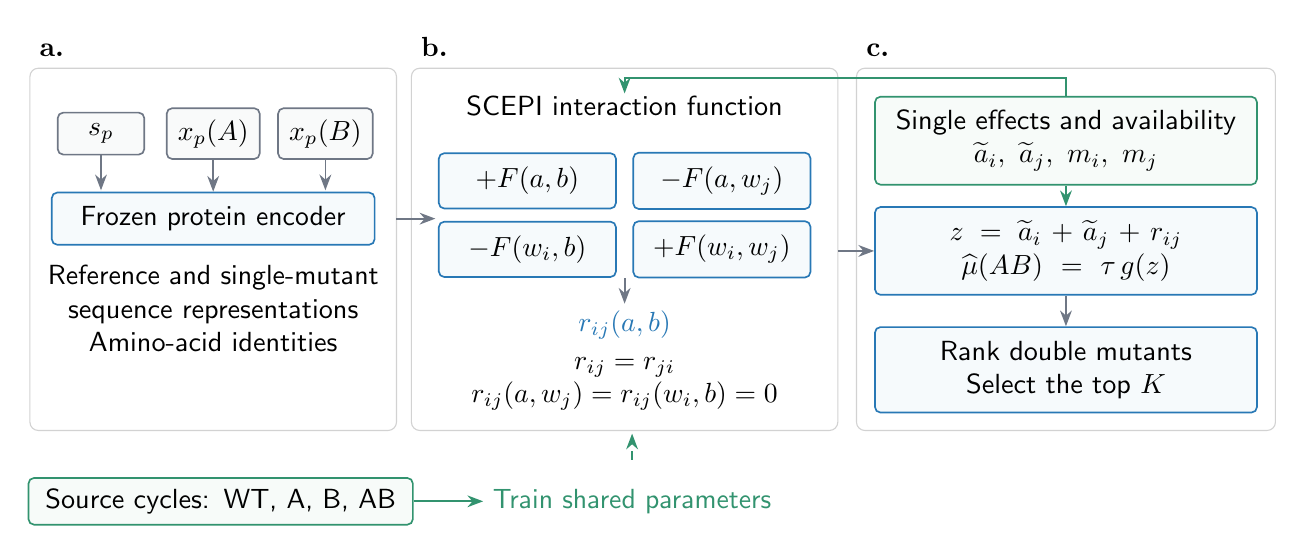
\begin{tikzpicture}[x=0.95cm,y=1cm,font=\sffamily\normalsize,
  modelbox/.style={draw=MethodBlue,fill=MethodBlue!4,rounded corners=2pt,
    line width=0.6pt,align=center,inner sep=5pt},
  inputbox/.style={draw=MethodGray,fill=MethodGray!4,rounded corners=2pt,
    line width=0.6pt,align=center,inner sep=4pt},
  signal/.style={-{Stealth[length=2mm]},draw=MethodGray,line width=0.65pt}]
\definecolor{MethodBlue}{HTML}{2878B5}
\definecolor{MethodGreen}{HTML}{32936F}
\definecolor{MethodGray}{HTML}{6F7785}
\draw[gray!35,rounded corners=3pt] (0,1.35) rectangle (4.9,5.95);
\draw[gray!35,rounded corners=3pt] (5.1,1.35) rectangle (10.8,5.95);
\draw[gray!35,rounded corners=3pt] (11.05,1.35) rectangle (16.65,5.95);
\node[anchor=south west,font=\bfseries\normalsize] at (0,5.98) {a.};
\node[anchor=south west,font=\bfseries\normalsize] at (5.1,5.98) {b.};
\node[anchor=south west,font=\bfseries\normalsize] at (11.05,5.98) {c.};
\node[inputbox,minimum width=1.1cm] (wt) at (0.95,5.12) {$s_p$};
\node[inputbox,minimum width=1.1cm] (singlea) at (2.45,5.12) {$x_p(A)$};
\node[inputbox,minimum width=1.1cm] (singleb) at (3.95,5.12) {$x_p(B)$};
\node[modelbox,minimum width=4.1cm,minimum height=0.65cm] (encoder) at (2.45,4.04) {Frozen protein encoder};
\draw[signal] (wt.south) -- (0.95,4.4);
\draw[signal] (singlea.south) -- (encoder.north);
\draw[signal] (singleb.south) -- (3.95,4.4);
\node[align=center,text width=4.2cm] at (2.45,2.9) {Reference and single-mutant\\sequence representations\\Amino-acid identities};
\node[align=center,text width=5.1cm] at (7.95,5.47) {SCEPI interaction function};
\node[modelbox,minimum width=2.25cm,minimum height=0.55cm] at (6.65,4.52) {$+F(a,b)$};
\node[modelbox,minimum width=2.25cm,minimum height=0.55cm] at (9.25,4.52) {$-F(a,w_j)$};
\node[modelbox,minimum width=2.25cm,minimum height=0.55cm] at (6.65,3.65) {$-F(w_i,b)$};
\node[modelbox,minimum width=2.25cm,minimum height=0.55cm] at (9.25,3.65) {$+F(w_i,w_j)$};
\draw[signal] (4.9,4.04) -- (5.42,4.04);
\draw[signal] (7.95,3.28) -- (7.95,2.96);
\node[text=MethodBlue,font=\normalsize] at (7.95,2.69) {$r_{ij}(a,b)$};
\node[align=center,font=\normalsize] at (7.95,1.94) {$r_{ij}=r_{ji}$\\$r_{ij}(a,w_j)=r_{ij}(w_i,b)=0$};
\node[modelbox,draw=MethodGreen,fill=MethodGreen!4,text width=4.5cm] (singles) at (13.85,5.03) {Single effects and availability\\$\widetilde a_i,\ \widetilde a_j,\ m_i,\ m_j$};
\draw[signal,draw=MethodGreen] (singles.north) -- (13.85,5.83) -- (7.95,5.83) -- (7.95,5.63);
\node[modelbox,text width=4.5cm,minimum height=0.87cm] (map) at (13.85,3.63) {$z=\widetilde a_i+\widetilde a_j+r_{ij}$\\$\widehat\mu(AB)=\tau\,g(z)$};
\draw[signal,draw=MethodGreen] (singles.south) -- (map.north);
\draw[signal] (10.8,3.63) -- (map.west);
\node[modelbox,text width=4.5cm,minimum height=0.7cm] (selection) at (13.85,2.12) {Rank double mutants\\Select the top $K$};
\draw[signal] (map.south) -- (selection.north);
\node[inputbox,draw=MethodGreen,fill=MethodGreen!4,text width=4.6cm] (quartets) at (2.55,0.45) {Source cycles: WT, A, B, AB};
\node[align=center,text=MethodGreen] (loss) at (8.05,0.45) {Train shared parameters};
\draw[signal,draw=MethodGreen] (quartets.east) -- (loss.west);
\draw[signal,draw=MethodGreen,dashed] (8.05,0.98) -- (8.05,1.31);
\end{tikzpicture}
\caption{SCEPI conditions shared interaction predictions on single-mutant measurements. (a) A frozen encoder supplies reference and mutation features from the reference sequence and its single mutants. (b) Calibrated single effects and their availability indicators condition every evaluation of the shared symmetric pair function. Subtraction around the double-mutant cycle enforces the reference constraints. (c) The same single effects enter the external sum before phenotype prediction. Double-mutant predictions then rank candidates at a fixed budget. Complete source cycles and source observations supervise SCEPI. Target double-mutant outcomes are reserved for evaluation.}
\label{fig:method}
\end{figure}

\subsection{Prediction problem}

Let $s_p$ be a reference protein and $M$ a set of substitutions at distinct sites. The predictor receives $s_p$, $M$, and the target measurements allowed by the information condition. It outputs the relative phenotype $\widehat\mu_p(M)$ and a candidate score. For two substitutions $A=(i,a)$ and $B=(j,b)$, the measured interaction is
\begin{equation}
\epsilon_p(A,B)=y_p(AB)-y_p(A)-y_p(B)+y_p(\varnothing).
\label{eq:observed}
\end{equation}
The four observations form a double-mutant cycle \citep{horovitz1996}. They share a reference background, assay condition, and phenotype scale. Stability is expressed as unfolding free energy, with positive changes indicating increased stability. Target single-mutant labels are available in the main compensation task. Target test double-mutant labels evaluate predictions and selected candidates.

\subsection{Mutation representations and calibrated single effects}

A frozen ESM-2 encoder $h$ supplies the sequence representations \citep{lin2023}. For substitution $A=(i,a)$, the endpoint representation contains $h_i(s_p)$, the local change $h_i(x_p(A))-h_i(s_p)$, amino-acid identities, and the pretrained substitution score. The single-effect head is shared across proteins and uses a reference subtraction,
\begin{equation}
a_i(a)=f_\phi(u_i(a))-f_\phi(u_i(w_i)),
\end{equation}
where $w_i$ is the reference residue, giving $a_i(w_i)=0$.

Available single-mutant effects enter through
\begin{equation}
\widetilde a_i(a)=a_i(a)+\omega m_i(a)\bigl[\mu_i^{\mathrm{obs}}(a)-a_i(a)\bigr],
\label{eq:calibration}
\end{equation}
where $\mu_i^{\mathrm{obs}}(a)=y_p(i,a)-y_p(\varnothing)$ is the measured effect relative to the same reference. The indicator $m_i(a)$ records label availability, and $\omega$ is selected on source-validation proteins. An observed zero remains an available label. The calibrated effects enter both the single-effect sum and the interaction network. Pair representations also include mutation-dependent cross-site context and sequence separation, defined with the structural variant in Appendix~\ref{app:parameterization}.

\subsection{Conditioning the shared interaction function}

For a candidate pair, collect the calibrated single effects and their availability indicators in
\begin{equation}
c_{ij}(a,b)=\bigl(\widetilde a_i(a),\widetilde a_j(b),m_i(a),m_j(b)\bigr).
\label{eq:conditioning}
\end{equation}
Together with the endpoint representations and site relation, $c_{ij}$ makes the shared network depend on measured effects from the target protein. Exchanging the endpoints also exchanges the entries of $c_{ij}$.

Let $\Psi_\theta(i,a;j,b\mid c_{ij})$ denote the ordered network. We average both orders:
\begin{equation}
F_\theta(i,a;j,b)=\tfrac12\bigl[\Psi_\theta(i,a;j,b\mid c_{ij})
+\Psi_\theta(j,b;i,a\mid c_{ji})\bigr].
\end{equation}
The conditioning inputs enter every evaluation of $F$. The pair output uses the same subtraction over the four states,
\begin{equation}
r_{ij}(a,b)=F(i,a;j,b)-F(i,a;j,w_j)-F(i,w_i;j,b)+F(i,w_i;j,w_j).
\label{eq:pair}
\end{equation}
Each call evaluates the specified amino-acid state. At a wild-type endpoint, the single effect and local representation change are zero. The context change caused by that endpoint at the other site is also removed.

The subtraction enforces symmetry, $r_{ij}(a,b)=r_{ji}(b,a)$, and zero reference effects, $r_{ij}(a,w_j)=r_{ij}(w_i,b)=0$. It also cancels every endpoint-only contribution, so replacing $F$ by $F+v_i(a)+v_j(b)+c$ leaves $r$ unchanged. We test the predictive contribution of these constraints against a matched direct head.

\subsection{Composition and phenotype prediction}

For a mutation set $M$, the latent effect sums single and pair contributions:
\begin{equation}
z_p(M)=\sum_{(i,a)\in M}\widetilde a_i(a)
+\sum_{\substack{(i,a),(j,b)\in M\\i<j}}r_{ij}(a,b).
\end{equation}
We predict $\widehat\mu_p(M)=\tau g(z_p(M))$, where $\tau>0$, $g(0)=0$, and $g'(0)=1$. The monotone map models global phenotype nonlinearity. Its parameterization is given in the appendix.

The model's interaction on the observed phenotype scale is always calculated from its four predictions:
\begin{equation}
\widehat\epsilon_p(A,B)=\widehat\mu_p(AB)-\widehat\mu_p(A)-\widehat\mu_p(B).
\label{eq:predicted}
\end{equation}
This contrast includes global phenotype nonlinearity and the learned pair contribution. It equals $r_{ij}$ under the identity map and unit scale. Appendix~\ref{app:parameterization} gives the decomposition.

\subsection{Learning from complete combination measurements}

After initialization on source single-mutant measurements, the single head, pair function, and phenotype map are fitted using source combinations. Source validation selects a phenotype likelihood or its combination with a Huber loss on the complete predicted residual. The likelihood retains point-valued and interval-valued observations. The residual loss balances proteins and site pairs.

To represent inference conditions, source training varies the permitted single-mutant information. Model configurations and the label-mixing weight are selected on source-validation proteins, excluding target homology groups from fitting and selection. Appendix~\ref{app:training} gives the criterion, observation model, and implementation. Residual-only and phenotype-only variants test the choice of objective.

\subsection{Compensatory candidate selection}

For a budget $K$, SCEPI selects the $K$ double mutants with the highest native phenotype predictions $\widehat\mu_p(AB)$. Recovery is measured relative to the better constituent single mutant,
\begin{equation}
R_p(A,B)=y_p(AB)-\max\{y_p(A),y_p(B)\}.
\end{equation}
A compensatory hit satisfies $R_p(A,B)\geq\delta$. The candidate task focuses on pairs whose two measured single effects are each at most $-\delta$. Here $K$ counts double-mutant measurements given the available single-mutant data.

To isolate interaction information, we fix the measured single-effect sum across methods. Each method $m$ ranks the same candidates by
\begin{equation}
s_m(A,B)=\mu_p^{\mathrm{obs}}(A)+\mu_p^{\mathrm{obs}}(B)+\widehat\epsilon_{m,p}(A,B).
\label{eq:selection}
\end{equation}
Each method retains its own four-prediction contrast, so scores differ through predicted nonadditivity. Native ranking evaluates the complete predictor; Equation~\eqref{eq:selection} isolates the selection value of its interaction predictions.

Uniform random selection samples $K$ candidates without replacement from the same protein-level pool. Its expected hit rate is the pool's hit fraction, and its expected mean recovery is the pool mean. Enrichment is the ratio of the model and random equal-protein mean hit rates. Appendix~\ref{app:random} gives the exact calculation and uncertainty analysis.

\section{Experimental setting}

The cDNA-display proteolysis measurements of Tsuboyama et al. provide stability data \citep{tsuboyama2023}. Among 182,663 accepted double mutants across 190 reference backgrounds, 127,892 form complete, point-valued cycles across 160 backgrounds and 488 site pairs. Retrospective evaluation requires all four measurements to lie strictly between $-1$ and 5 kcal/mol. Training additionally retains interval-valued observations through the observation likelihood.

In the primary S-all evaluation, all permitted target single-mutant labels are available and every target double-mutant label is withheld from fitting. We score all accepted double mutants in held-out homology groups. Groups use 30\% sequence identity and at least 80\% bidirectional coverage, keeping related reference backgrounds together. Annotated family relations further merge groups. Source training and validation exclude the outer test partition. Coverage is recorded separately for homology groups and annotated families.

We compare independently trained additive and global nonlinear models with ThermoMPNN-D, Kermut, StabilityArc + Kermut, mean ridge, and mean MLP. The global control keeps the monotone map and omits the pair term. Mean ridge and mean MLP fit ridge regression or a multilayer perceptron (MLP) to averaged mutation representations. For source-trained baselines, retraining uses the same source partitions and source-validation checkpoint selection. StabilityArc scores provide Kermut's prior mean during target calibration \citep{feller2026,groth2024}. All methods score the same candidates with zero target double-mutant labels. Their architectures, supervision, adaptation, and structural inputs are specified in Appendices~\ref{app:training} and~\ref{app:stabilityarc}.

Prediction error is measured by root mean squared error (RMSE). The phenotype cohort contains 159 proteins from 51 homology groups, each with at least 30 point-valued target measurements. Residual evaluation requires at least 30 complete, in-range cycles and retains 155 proteins from the same 51 groups. For compensation selection, we require at least 100 eligible candidates and reference stability at most 4.5 kcal/mol. This gives 120 proteins from 44 groups. Candidate budgets are $K\in\{1,3,10,30\}$, with recovery threshold $\delta=0.5$ kcal/mol.

Metrics are computed within protein, averaged over matched repetitions, and then averaged equally across proteins. Source-validation measurements determine hyperparameters and label-mixing weights.

Measurement-boundary analysis uses each cycle's smallest distance from either assay limit. Margins of 0.25 and 0.5 kcal/mol retain 120 and 115 compensation proteins, respectively; the latter covers 43 groups. The designated site-pair subset and target combination adaptation are evaluated separately. Statistical and repetition details appear in the appendix.

We vary target-label availability in additional information conditions. Z permits no target measurements; S32 and S128 permit the reference and the specified number of single-mutant labels. The C conditions also permit 128, 512, 2,048, or all available training double-mutant labels, excluding held-out test site pairs from target combination fitting. Separate adaptation experiments cover six functional assays and nine FLIP2 split protocols \citep{didi2026}. Appendix~\ref{app:externaladaptation} defines their measurement units, model variants, and evaluation populations.

\section{Results}
\interlinepenalty=10000

\subsection{Measured single effects improve interaction prediction and selection}

Measured inputs within the pair function reduce residual RMSE by 23.0\% under the primary grouping and 25.7\% under the stricter grouping (Table~\ref{tab:conditioning}; Figure~\ref{fig:components}). Native top-10 hit rates rise by 2.98 and 3.00 percentage points. Both mean gains are positive in every matched training repetition under each grouping. The controls independently vary numerical values and availability indicators inside $F$. Each is refitted with the same external calibration rule, capacity, initialization, source samples, objective, and stopping rule. All comparisons retain 155 residual-evaluation proteins and 120 compensation proteins.

Numerical values retain residual reductions of 0.172 and 0.193 kcal/mol when indicators are removed. Their native hit-rate gains are 3.20 and 2.97 percentage points. Adding indicators to measured values yields smaller residual reductions of 0.004 and 0.016 kcal/mol, with hit-rate changes of $-0.22$ and 0.03 points. Indicators alone leave residual error at 0.772 and 0.817 kcal/mol. The principal prediction benefit comes from the measured numerical effects.

Fixing the measured single-effect sum preserves hit-rate gains of 3.08 and 3.02 percentage points over the input-removal control. At the 0.5 kcal/mol measurement margin, these gains are 3.11 and 3.13 points. The pair network therefore uses measured effects to improve selection even when the external single-effect sum is identical.

\begin{table}[!tbp]
\centering
\setlength{\tabcolsep}{4pt}
\caption{Matched pair-function comparisons under 30\% and 25\% homology grouping. Residual prediction covers 155 proteins; native top-10 selection covers 120. Values only removes indicators from $F$. Indicators only retains indicators with predicted values. Predicted singles uses predicted values and zero indicators. Every control retains external calibration. The direct head retains both measured inputs and replaces cycle subtraction with the same network's direct output.}
\label{tab:conditioning}
\begin{tabular}{lrrrr}
\toprule
 & \multicolumn{2}{c}{Residual RMSE (kcal/mol)} & \multicolumn{2}{c}{Native hit rate (\%)} \\
Pair function & 30\% & 25\% & 30\% & 25\% \\
\midrule
SCEPI & 0.590 & 0.604 & 11.22 & 11.15 \\
Values only & 0.595 & 0.621 & 11.43 & 11.12 \\
Indicators only & 0.772 & 0.817 & 8.10 & 7.95 \\
Predicted singles & 0.767 & 0.814 & 8.23 & 8.15 \\
Direct residual head & 0.632 & 0.630 & 10.53 & 11.38 \\
\bottomrule
\end{tabular}
\end{table}

\begin{table}[t]
\centering
\setlength{\tabcolsep}{4pt}
\caption{Full-target prediction and native top-10 compensation selection in held-out homology groups. Phenotype, residual, and selection cohorts contain 159, 155, and 120 proteins. RMSE uses kcal/mol. Values are equal-protein means over matched repetitions. Enrichment is relative to uniform random selection from the same candidates. All models receive zero target double-mutant training labels.}
\label{tab:diagnostic}
\begin{tabular}{lrrrrr}
\toprule
Predictor & Phenotype & Residual & Hit rate & Recovery & Enrichment \\
 & RMSE & RMSE & (\%) & (kcal/mol) & ($\times$) \\
\midrule
SCEPI & \textbf{0.651} & \textbf{0.590} & 11.22 & \textbf{$-0.262$} & 4.27 \\
ThermoMPNN-D & 0.777 & 0.805 & 7.07 & $-0.440$ & 2.69 \\
Kermut & 0.798 & 0.847 & 5.40 & $-0.458$ & 2.05 \\
StabilityArc + Kermut & 0.815 & 0.853 & 8.75 & $-0.344$ & 3.33 \\
Global nonlinear & 0.911 & 0.635 & 4.45 & $-0.437$ & 1.69 \\
Additive & 0.893 & 1.091 & 6.38 & $-0.387$ & 2.43 \\
Mean MLP & 1.405 & 0.966 & 10.07 & $-0.413$ & 3.83 \\
Mean ridge & 1.328 & 1.002 & \textbf{11.42} & $-0.354$ & \textbf{4.34} \\
Uniform random & --- & --- & 2.63 & $-0.900$ & 1.00 \\
\bottomrule
\end{tabular}
\end{table}

\subsection{The conditional predictor improves compensatory candidate discovery}

At a budget of $K=10$ candidates, native SCEPI predictions yield an 11.22\% mean compensation hit rate (Table~\ref{tab:diagnostic}). ThermoMPNN-D reaches 7.07\%, Kermut 5.40\%, and the global nonlinear model 4.45\%. The corresponding hit-rate gains are 4.15, 5.82, and 6.77 percentage points, with mean recovery gains of 0.178, 0.195, and 0.175 kcal/mol. Higher recovery occurs in 86 of 120 proteins against ThermoMPNN-D and 94 of 120 against Kermut. StabilityArc + Kermut reaches an 8.75\% top-10 hit rate. Against this method, SCEPI gains 2.47 percentage points in hit rate and 0.082 kcal/mol in mean recovery, with higher recovery in 71 of 120 proteins. Both predictors learn pair effects across source proteins and use target single-mutant measurements. Figure~\ref{fig:compensation} shows the budget curves and protein-level hit-rate differences.

Mean selected recovery favors SCEPI over all seven baselines at every evaluated budget. At $K=10$, mean ridge has a slightly higher hit rate of 11.42\%, compared with SCEPI's 11.22\% and mean MLP's 10.07\%. SCEPI's recovery advantage over mean ridge is 0.092 kcal/mol. Relative to the additive model's 6.38\% hit rate, SCEPI gains 4.83 percentage points and 0.125 kcal/mol mean recovery.

Uniform random selection from the same 79,564 candidates across 120 proteins has an expected equal-protein hit rate of 2.63\% and mean recovery of $-0.900$ kcal/mol. At $K=10$, SCEPI enriches hits 4.27-fold, gaining 8.59 percentage points in hit rate and 0.637 kcal/mol in mean recovery. Enrichment decreases from 5.26 to 4.80, 4.27, and 3.28 as the budget increases through 1, 3, 10, and 30 candidates (Figure~\ref{fig:compensation}a,b).

\begin{figure}[!tbp]
\centering
% Self-contained PGFPlots fragment generated from the verified family30 S-all selection tables.
% The 120 protein-level coordinates for each control in panels c and d are embedded explicitly.
% Self-contained PGFPlots fragment generated from the verified family30 S-all selection tables.
% The 120 protein-level coordinates for each control in panels c and d are embedded explicitly.
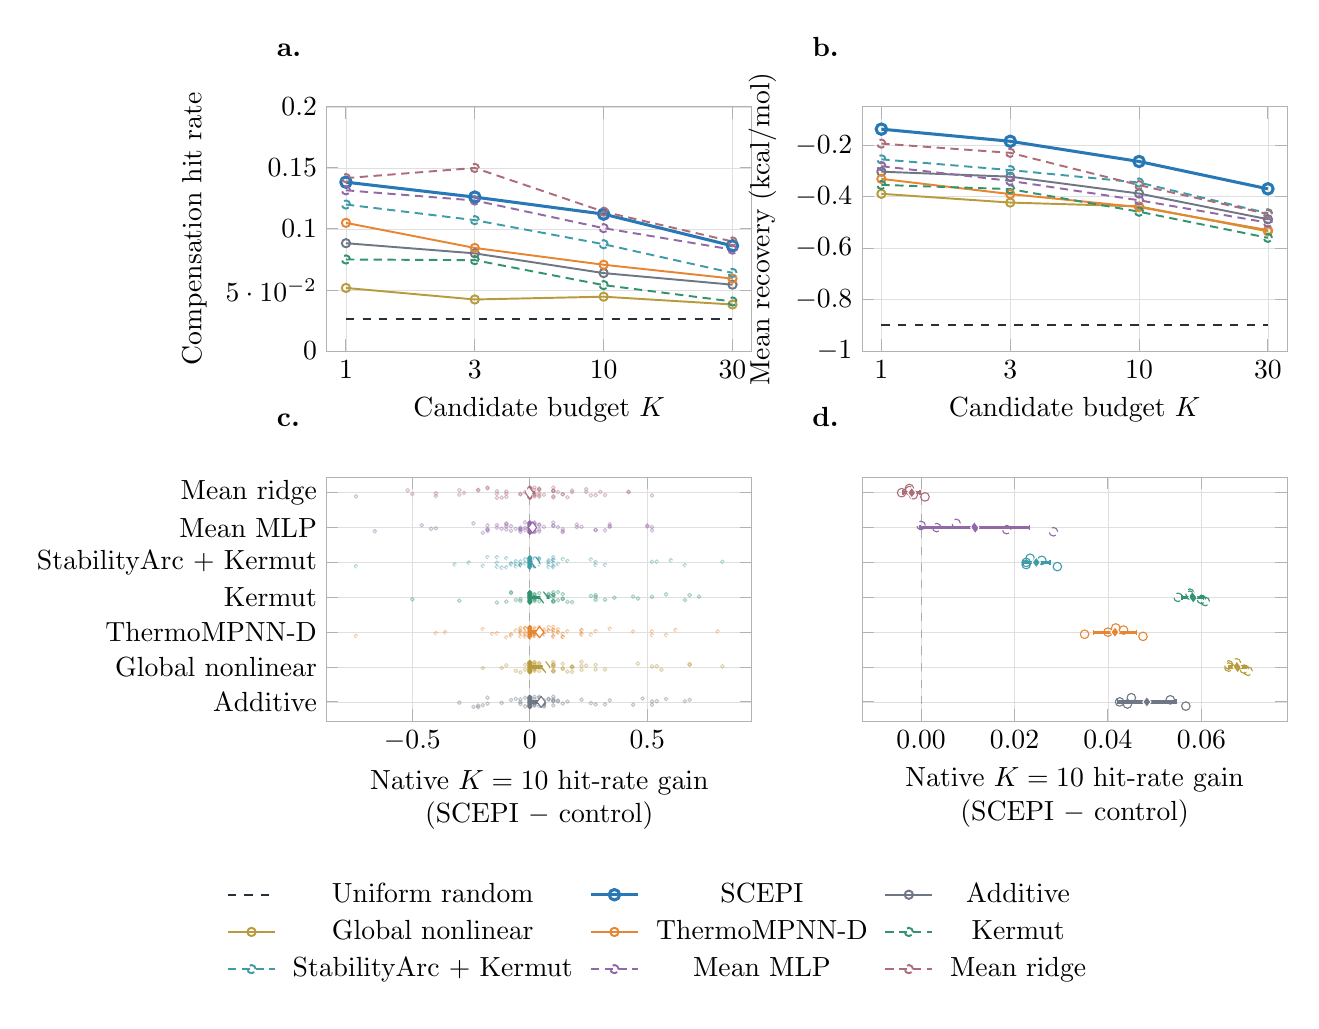
\begin{tikzpicture}
\definecolor{SharedBlue}{HTML}{2878B5}
\definecolor{AdditiveGray}{HTML}{6F7785}
\definecolor{GlobalGold}{HTML}{B89B3C}
\definecolor{ThermoOrange}{HTML}{E68632}
\definecolor{KermutGreen}{HTML}{32936F}
\definecolor{StabilityArcTeal}{HTML}{3F9BA8}
\definecolor{MeanMlpPurple}{HTML}{9368A6}
\definecolor{MeanRidgeRose}{HTML}{AC6D79}
\definecolor{CompensationDark}{HTML}{26313A}
\pgfplotsset{compat=1.18}
\begin{groupplot}[
  group style={group size=2 by 2, horizontal sep=14mm, vertical sep=16mm},
  width=54mm, height=31mm, scale only axis,
  tick label style={font=\normalsize}, label style={font=\normalsize},
  axis line style={draw={gray!60}, line width=0.35pt},
  grid=major, grid style={draw={gray!25}, line width=0.25pt},
  tick style={draw={gray!60}, line width=0.35pt},
  every axis plot/.append style={line join=round},
]
\nextgroupplot[
  title={\textbf{a.}}, title style={at={(axis description cs:-0.14,1.10)}, anchor=south west, font=\normalsize},
  ylabel={Compensation hit rate}, xmin=-0.15, xmax=3.15, ymin=0, ymax=0.2,
  xtick={0,1,2,3}, xticklabels={1,3,10,30}, xlabel={Candidate budget $K$},
  legend to name=compensationdiscoverylegend, legend style={draw=none, legend columns=3, font=\normalsize, column sep=4pt, row sep=1pt},
]
  \addplot+[color=CompensationDark, dashed, line width=0.7pt, mark=none] coordinates {(0,0.026290797875) (1,0.026290797875) (2,0.026290797875) (3,0.026290797875)};
  \addlegendentry{Uniform random}
  \addplot+[color=SharedBlue, line width=1.1pt, mark=o, mark size=1.9pt, mark options={fill=white}] coordinates {(0,0.138333333333) (1,0.126111111111) (2,0.112166666667) (3,0.086166666667)};
  \addlegendentry{SCEPI}
  \addplot+[color=AdditiveGray, line width=0.7pt, mark=o, mark size=1.5pt, mark options={fill=white}] coordinates {(0,0.088333333333) (1,0.08) (2,0.063833333333) (3,0.054333333333)};
  \addlegendentry{Additive}
  \addplot+[color=GlobalGold, line width=0.7pt, mark=o, mark size=1.5pt, mark options={fill=white}] coordinates {(0,0.051666666667) (1,0.042222222222) (2,0.0445) (3,0.038111111111)};
  \addlegendentry{Global nonlinear}
  \addplot+[color=ThermoOrange, line width=0.7pt, mark=o, mark size=1.5pt, mark options={fill=white}] coordinates {(0,0.105) (1,0.084444444444) (2,0.070666666667) (3,0.059333333333)};
  \addlegendentry{ThermoMPNN-D}
  \addplot+[color=KermutGreen, line width=0.7pt, mark=o, mark size=1.5pt, mark options={fill=white}] coordinates {(0,0.075) (1,0.074444444444) (2,0.054) (3,0.040555555556)};
  \addlegendentry{Kermut}
  \addplot+[color=StabilityArcTeal, line width=0.7pt, mark=o, mark size=1.5pt, mark options={fill=white}] coordinates {(0,0.12) (1,0.107222222222) (2,0.0875) (3,0.064)};
  \addlegendentry{StabilityArc + Kermut}
  \addplot+[color=MeanMlpPurple, line width=0.7pt, mark=o, mark size=1.5pt, mark options={fill=white}] coordinates {(0,0.131666666667) (1,0.123333333333) (2,0.100666666667) (3,0.083055555556)};
  \addlegendentry{Mean MLP}
  \addplot+[color=MeanRidgeRose, line width=0.7pt, mark=o, mark size=1.5pt, mark options={fill=white}] coordinates {(0,0.141666666667) (1,0.15) (2,0.114166666667) (3,0.089722222222)};
  \addlegendentry{Mean ridge}
\nextgroupplot[
  title={\textbf{b.}}, title style={at={(axis description cs:-0.14,1.10)}, anchor=south west, font=\normalsize},
  ylabel={Mean recovery (kcal/mol)}, xmin=-0.15, xmax=3.15, ymin=-1, ymax=-0.05,
  xtick={0,1,2,3}, xticklabels={1,3,10,30}, xlabel={Candidate budget $K$},
]
  \addplot+[color=CompensationDark, dashed, line width=0.7pt, mark=none] coordinates {(0,-0.899620802378) (1,-0.899620802378) (2,-0.899620802378) (3,-0.899620802378)};
  \addplot+[color=SharedBlue, line width=1.1pt, mark=o, mark size=1.9pt, mark options={fill=white}] coordinates {(0,-0.136561651345) (1,-0.183766769106) (2,-0.262424771069) (3,-0.368884227779)};
  \addplot+[color=AdditiveGray, line width=0.7pt, mark=o, mark size=1.5pt, mark options={fill=white}] coordinates {(0,-0.302084650293) (1,-0.321524772155) (2,-0.387166470503) (3,-0.487273898384)};
  \addplot+[color=GlobalGold, line width=0.7pt, mark=o, mark size=1.5pt, mark options={fill=white}] coordinates {(0,-0.388216650076) (1,-0.422298604783) (2,-0.437107837454) (3,-0.534390046825)};
  \addplot+[color=ThermoOrange, line width=0.7pt, mark=o, mark size=1.5pt, mark options={fill=white}] coordinates {(0,-0.330163027865) (1,-0.389229391704) (2,-0.439989897835) (3,-0.529539584243)};
  \addplot+[color=KermutGreen, line width=0.7pt, mark=o, mark size=1.5pt, mark options={fill=white}] coordinates {(0,-0.353548993619) (1,-0.369886322374) (2,-0.457853837912) (3,-0.55944331145)};
  \addplot+[color=StabilityArcTeal, line width=0.7pt, mark=o, mark size=1.5pt, mark options={fill=white}] coordinates {(0,-0.254131768125) (1,-0.295844002785) (2,-0.344276096869) (3,-0.463920626297)};
  \addplot+[color=MeanMlpPurple, line width=0.7pt, mark=o, mark size=1.5pt, mark options={fill=white}] coordinates {(0,-0.280689535249) (1,-0.337920062969) (2,-0.413362681969) (3,-0.500511039679)};
  \addplot+[color=MeanRidgeRose, line width=0.7pt, mark=o, mark size=1.5pt, mark options={fill=white}] coordinates {(0,-0.192865610602) (1,-0.228774345629) (2,-0.354448706602) (3,-0.466990646203)};
\nextgroupplot[
  xlabel={Native $K=10$ hit-rate gain\\(SCEPI $-$ control)},
  xlabel style={align=center},
  ymin=-0.55, ymax=6.45, xmin=-0.8648, xmax=0.9448,
  ytick={0,1,2,3,4,5,6}, yticklabels={Additive,Global nonlinear,ThermoMPNN-D,Kermut,StabilityArc + Kermut,Mean MLP,Mean ridge},
  title={\textbf{c.}}, title style={at={(axis description cs:-0.14,1.10)}, anchor=south west, font=\normalsize},
]
  \addplot+[only marks, mark=o, mark size=0.65pt, mark options={draw=AdditiveGray, fill=white, opacity=0.42}] coordinates {(-0.22,-0.15) (0,-0.147478991597) (0,-0.144957983193) (0,-0.14243697479) (-0.24,-0.139915966387) (0,-0.137394957983) (0,-0.13487394958) (0.06,-0.132352941176) (-0.02,-0.129831932773) (0,-0.12731092437) (0,-0.124789915966) (0,-0.122268907563) (0,-0.11974789916) (0,-0.117226890756) (0,-0.114705882353) (0.04,-0.11218487395) (0.02,-0.109663865546) (-0.22,-0.107142857143) (0.06,-0.104621848739) (0.1,-0.102100840336) (0,-0.099579831933) (-0.2,-0.097058823529) (0,-0.094537815126) (0,-0.092016806723) (0,-0.089495798319) (0,-0.086974789916) (0,-0.084453781513) (0.52,-0.081932773109) (0.44,-0.079411764706) (0.02,-0.076890756303) (0,-0.074369747899) (0.28,-0.071848739496) (0.32,-0.069327731092) (0,-0.066806722689) (0,-0.064285714286) (-0.04,-0.061764705882) (0,-0.059243697479) (0.06,-0.056722689076) (0.02,-0.054201680672) (0.06,-0.051680672269) (-0.18,-0.049159663866) (0.14,-0.046638655462) (0.06,-0.044117647059) (0,-0.041596638655) (0,-0.039075630252) (0.26,-0.036554621849) (0,-0.034033613445) (0.06,-0.031512605042) (-0.12,-0.028991596639) (0,-0.026470588235) (0.02,-0.023949579832) (-0.3,-0.021428571429) (0,-0.018907563025) (0,-0.016386554622) (0,-0.013865546218) (0.02,-0.011344537815) (0,-0.008823529412) (0,-0.006302521008) (-0.04,-0.003781512605) (0.04,-0.001260504202) (0,0.001260504202) (0,0.003781512605) (0,0.006302521008) (0,0.008823529412) (0.16,0.011344537815) (0.12,0.013865546218) (0.52,0.016386554622) (0.66,0.018907563025) (0.54,0.021428571429) (0.1,0.023949579832) (0,0.026470588235) (0.1,0.028991596639) (0,0.031512605042) (0,0.034033613445) (0,0.036554621849) (0,0.039075630252) (0.12,0.041596638655) (0.34,0.044117647059) (0.06,0.046638655462) (0,0.049159663866) (-0.08,0.051680672269) (0,0.054201680672) (0,0.056722689076) (0,0.059243697479) (0.68,0.061764705882) (0.22,0.064285714286) (0.08,0.066806722689) (0,0.069327731092) (-0.04,0.071848739496) (0.1,0.074369747899) (0,0.076890756303) (0.02,0.079411764706) (0,0.081932773109) (0.58,0.084453781513) (-0.06,0.086974789916) (0,0.089495798319) (0.08,0.092016806723) (0,0.094537815126) (0.48,0.097058823529) (0,0.099579831933) (0,0.102100840336) (0,0.104621848739) (0,0.107142857143) (0,0.109663865546) (0,0.11218487395) (0,0.114705882353) (0.04,0.117226890756) (-0.02,0.11974789916) (-0.18,0.122268907563) (0,0.124789915966) (0,0.12731092437) (0,0.129831932773) (0,0.132352941176) (0,0.13487394958) (0,0.137394957983) (0,0.139915966387) (0,0.14243697479) (0.04,0.144957983193) (0.02,0.147478991597) (0.1,0.15)};
  \addplot[color=AdditiveGray, line width=1.25pt] coordinates {(0,0) (0.06,0)};
  \addplot[color=CompensationDark, line width=0.5pt] coordinates {(0,-0.1) (0,0.1)};
  \addplot+[only marks, mark=diamond*, mark size=2.0pt, mark options={draw=AdditiveGray, fill=white}] coordinates {(0.048333333333,0)};
  \addplot+[only marks, mark=o, mark size=0.65pt, mark options={draw=GlobalGold, fill=white, opacity=0.42}] coordinates {(-0.04,0.85) (0,0.852521008403) (0,0.855042016807) (0,0.85756302521) (0.18,0.860084033613) (0,0.862605042017) (0.1,0.86512605042) (0.16,0.867647058824) (0,0.870168067227) (0,0.87268907563) (0,0.875210084034) (0,0.877731092437) (0,0.88025210084) (0,0.882773109244) (0,0.885294117647) (0.04,0.88781512605) (0.02,0.890336134454) (-0.06,0.892857142857) (0.1,0.895378151261) (0.1,0.897899159664) (0,0.900420168067) (0,0.902941176471) (0,0.905462184874) (0,0.907983193277) (0,0.910504201681) (0,0.913025210084) (0,0.915546218487) (0.22,0.918067226891) (0.56,0.920588235294) (-0.02,0.923109243697) (0.02,0.925630252101) (0.28,0.928151260504) (0.32,0.930672268908) (0,0.933193277311) (0,0.935714285714) (0,0.938235294118) (0,0.940756302521) (0.06,0.943277310924) (0.02,0.945798319328) (0.06,0.948319327731) (0,0.950840336134) (0.14,0.953361344538) (0.14,0.955882352941) (0,0.958403361345) (0,0.960924369748) (0.06,0.963445378151) (0,0.965966386555) (0.06,0.968487394958) (-0.2,0.971008403361) (0,0.973529411765) (0.02,0.976050420168) (-0.12,0.978571428571) (0,0.981092436975) (0,0.983613445378) (0,0.986134453782) (0.18,0.988655462185) (0,0.991176470588) (0,0.993697478992) (0.02,0.996218487395) (0,0.998739495798) (0,1.001260504202) (0,1.003781512605) (0,1.006302521008) (0.1,1.008823529412) (0.18,1.011344537815) (0.18,1.013865546218) (0.52,1.016386554622) (0.82,1.018907563025) (0.54,1.021428571429) (0,1.023949579832) (0,1.026470588235) (0.22,1.028991596639) (0,1.031512605042) (0.1,1.034033613445) (0,1.036554621849) (0,1.039075630252) (0.24,1.041596638655) (0,1.044117647059) (0,1.046638655462) (-0.1,1.049159663866) (0,1.051680672269) (0,1.054201680672) (0,1.056722689076) (0.02,1.059243697479) (0.68,1.061764705882) (0.28,1.064285714286) (-0.02,1.066806722689) (0,1.069327731092) (0.1,1.071848739496) (0.1,1.074369747899) (0,1.076890756303) (0.02,1.079411764706) (0,1.081932773109) (0.68,1.084453781513) (0.04,1.086974789916) (0,1.089495798319) (0.14,1.092016806723) (0,1.094537815126) (0.46,1.097058823529) (0,1.099579831933) (0,1.102100840336) (0,1.104621848739) (0,1.107142857143) (0,1.109663865546) (0,1.11218487395) (0,1.114705882353) (0.04,1.117226890756) (0,1.11974789916) (0.02,1.122268907563) (0,1.124789915966) (0,1.12731092437) (0,1.129831932773) (0,1.132352941176) (0,1.13487394958) (0,1.137394957983) (0,1.139915966387) (0,1.14243697479) (0.1,1.144957983193) (0.02,1.147478991597) (0.22,1.15)};
  \addplot[color=GlobalGold, line width=1.25pt] coordinates {(0,1) (0.07,1)};
  \addplot[color=CompensationDark, line width=0.5pt] coordinates {(0,0.9) (0,1.1)};
  \addplot+[only marks, mark=diamond*, mark size=2.0pt, mark options={draw=GlobalGold, fill=white}] coordinates {(0.067666666667,1)};
  \addplot+[only marks, mark=o, mark size=0.65pt, mark options={draw=ThermoOrange, fill=white, opacity=0.42}] coordinates {(-0.1,1.85) (0,1.852521008403) (0,1.855042016807) (0,1.85756302521) (0.14,1.860084033613) (0,1.862605042017) (0.1,1.86512605042) (0.14,1.867647058824) (-0.02,1.870168067227) (0,1.87268907563) (0,1.875210084034) (-0.04,1.877731092437) (0,1.88025210084) (0,1.882773109244) (0,1.885294117647) (0.04,1.88781512605) (0.02,1.890336134454) (-0.74,1.892857142857) (0.02,1.895378151261) (0.1,1.897899159664) (0,1.900420168067) (-0.08,1.902941176471) (0,1.905462184874) (0,1.907983193277) (0,1.910504201681) (0,1.913025210084) (0,1.915546218487) (0.52,1.918067226891) (0.58,1.920588235294) (0.04,1.923109243697) (0.02,1.925630252101) (0.22,1.928151260504) (0.26,1.930672268908) (0,1.933193277311) (0,1.935714285714) (-0.02,1.938235294118) (-0.08,1.940756302521) (0.06,1.943277310924) (0.02,1.945798319328) (0.06,1.948319327731) (-0.16,1.950840336134) (0.04,1.953361344538) (0.14,1.955882352941) (0,1.958403361345) (0,1.960924369748) (0.22,1.963445378151) (0,1.965966386555) (-0.14,1.968487394958) (-0.4,1.971008403361) (0,1.973529411765) (0.02,1.976050420168) (-0.04,1.978571428571) (0,1.981092436975) (0,1.983613445378) (-0.02,1.986134453782) (0.12,1.988655462185) (0,1.991176470588) (0,1.993697478992) (-0.36,1.996218487395) (0.1,1.998739495798) (0,2.001260504202) (0,2.003781512605) (-0.04,2.006302521008) (0,2.008823529412) (0.12,2.011344537815) (0.06,2.013865546218) (0.44,2.016386554622) (0.8,2.018907563025) (0.52,2.021428571429) (0.16,2.023949579832) (0,2.026470588235) (0.28,2.028991596639) (0,2.031512605042) (0,2.034033613445) (0,2.036554621849) (0,2.039075630252) (0.08,2.041596638655) (0.22,2.044117647059) (0.08,2.046638655462) (-0.06,2.049159663866) (-0.04,2.051680672269) (0,2.054201680672) (0,2.056722689076) (0.1,2.059243697479) (0.62,2.061764705882) (0.22,2.064285714286) (0.04,2.066806722689) (0,2.069327731092) (0.06,2.071848739496) (0.1,2.074369747899) (0,2.076890756303) (0.02,2.079411764706) (0,2.081932773109) (0.12,2.084453781513) (0,2.086974789916) (0,2.089495798319) (-0.2,2.092016806723) (0,2.094537815126) (0.34,2.097058823529) (0,2.099579831933) (0,2.102100840336) (0,2.104621848739) (-0.02,2.107142857143) (0,2.109663865546) (0,2.11218487395) (0,2.114705882353) (-0.02,2.117226890756) (-0.04,2.11974789916) (0.02,2.122268907563) (0,2.124789915966) (0,2.12731092437) (0,2.129831932773) (0,2.132352941176) (0,2.13487394958) (0,2.137394957983) (0,2.139915966387) (0,2.14243697479) (0.04,2.144957983193) (0.08,2.147478991597) (0.1,2.15)};
  \addplot[color=ThermoOrange, line width=1.25pt] coordinates {(0,2) (0.06,2)};
  \addplot[color=CompensationDark, line width=0.5pt] coordinates {(0,1.9) (0,2.1)};
  \addplot+[only marks, mark=diamond*, mark size=2.0pt, mark options={draw=ThermoOrange, fill=white}] coordinates {(0.0415,2)};
  \addplot+[only marks, mark=o, mark size=0.65pt, mark options={draw=KermutGreen, fill=white, opacity=0.42}] coordinates {(-0.14,2.85) (0,2.852521008403) (0,2.855042016807) (0,2.85756302521) (0.18,2.860084033613) (0,2.862605042017) (0.1,2.86512605042) (0.16,2.867647058824) (0,2.870168067227) (0,2.87268907563) (0,2.875210084034) (-0.1,2.877731092437) (0,2.88025210084) (0,2.882773109244) (0,2.885294117647) (0.04,2.88781512605) (0.02,2.890336134454) (-0.04,2.892857142857) (0.1,2.895378151261) (0.1,2.897899159664) (0,2.900420168067) (-0.3,2.902941176471) (0,2.905462184874) (0,2.907983193277) (0,2.910504201681) (0,2.913025210084) (0,2.915546218487) (0.12,2.918067226891) (0.66,2.920588235294) (-0.06,2.923109243697) (0.02,2.925630252101) (0.28,2.928151260504) (0.32,2.930672268908) (0,2.933193277311) (0,2.935714285714) (0,2.938235294118) (-0.5,2.940756302521) (0.06,2.943277310924) (0.02,2.945798319328) (-0.04,2.948319327731) (0,2.950840336134) (0.14,2.953361344538) (0.14,2.955882352941) (0,2.958403361345) (0,2.960924369748) (0.46,2.963445378151) (0,2.965966386555) (0.06,2.968487394958) (0,2.971008403361) (0,2.973529411765) (0.02,2.976050420168) (0,2.978571428571) (0,2.981092436975) (0,2.983613445378) (0,2.986134453782) (0.36,2.988655462185) (0,2.991176470588) (0,2.993697478992) (0.02,2.996218487395) (0.1,2.998739495798) (0,3.001260504202) (0,3.003781512605) (0,3.006302521008) (0.08,3.008823529412) (0.28,3.011344537815) (0.08,3.013865546218) (0.52,3.016386554622) (0.72,3.018907563025) (0.44,3.021428571429) (0,3.023949579832) (0,3.026470588235) (0.02,3.028991596639) (0,3.031512605042) (0,3.034033613445) (0,3.036554621849) (0,3.039075630252) (0.26,3.041596638655) (0,3.044117647059) (0,3.046638655462) (0,3.049159663866) (0,3.051680672269) (0,3.054201680672) (0,3.056722689076) (0.1,3.059243697479) (0.68,3.061764705882) (0.28,3.064285714286) (0.08,3.066806722689) (0,3.069327731092) (0.1,3.071848739496) (0.1,3.074369747899) (0,3.076890756303) (0.02,3.079411764706) (0,3.081932773109) (0.58,3.084453781513) (0.02,3.086974789916) (0,3.089495798319) (0.14,3.092016806723) (0,3.094537815126) (0.08,3.097058823529) (0,3.099579831933) (0,3.102100840336) (0,3.104621848739) (0,3.107142857143) (0,3.109663865546) (0,3.11218487395) (0,3.114705882353) (0.04,3.117226890756) (0,3.11974789916) (-0.08,3.122268907563) (0,3.124789915966) (0,3.12731092437) (0,3.129831932773) (0,3.132352941176) (0,3.13487394958) (0,3.137394957983) (0,3.139915966387) (0,3.14243697479) (0.1,3.144957983193) (-0.08,3.147478991597) (0.12,3.15)};
  \addplot[color=KermutGreen, line width=1.25pt] coordinates {(0,3) (0.08,3)};
  \addplot[color=CompensationDark, line width=0.5pt] coordinates {(0,2.9) (0,3.1)};
  \addplot+[only marks, mark=diamond*, mark size=2.0pt, mark options={draw=KermutGreen, fill=white}] coordinates {(0.058166666667,3)};
  \addplot+[only marks, mark=o, mark size=0.65pt, mark options={draw=StabilityArcTeal, fill=white, opacity=0.42}] coordinates {(-0.12,3.85) (0,3.852521008403) (0,3.855042016807) (0,3.85756302521) (-0.1,3.860084033613) (0,3.862605042017) (0.1,3.86512605042) (0.08,3.867647058824) (0,3.870168067227) (0,3.87268907563) (0,3.875210084034) (-0.14,3.877731092437) (0,3.88025210084) (0,3.882773109244) (0,3.885294117647) (-0.06,3.88781512605) (0.02,3.890336134454) (-0.74,3.892857142857) (0.02,3.895378151261) (0.1,3.897899159664) (0,3.900420168067) (-0.2,3.902941176471) (0,3.905462184874) (0,3.907983193277) (0,3.910504201681) (0,3.913025210084) (0,3.915546218487) (-0.04,3.918067226891) (0.66,3.920588235294) (-0.04,3.923109243697) (0.02,3.925630252101) (0.28,3.928151260504) (0.32,3.930672268908) (0,3.933193277311) (0,3.935714285714) (0,3.938235294118) (-0.32,3.940756302521) (0.04,3.943277310924) (-0.08,3.945798319328) (-0.04,3.948319327731) (0,3.950840336134) (0.08,3.953361344538) (0.12,3.955882352941) (0,3.958403361345) (0,3.960924369748) (-0.06,3.963445378151) (0,3.965966386555) (0.02,3.968487394958) (-0.08,3.971008403361) (0,3.973529411765) (0.02,3.976050420168) (-0.02,3.978571428571) (0,3.981092436975) (0,3.983613445378) (0,3.986134453782) (-0.14,3.988655462185) (0,3.991176470588) (0,3.993697478992) (-0.26,3.996218487395) (0.1,3.998739495798) (0,4.001260504202) (0,4.003781512605) (0,4.006302521008) (0,4.008823529412) (0.28,4.011344537815) (0.08,4.013865546218) (0.52,4.016386554622) (0.82,4.018907563025) (0.54,4.021428571429) (0,4.023949579832) (0,4.026470588235) (-0.04,4.028991596639) (0,4.031512605042) (-0.06,4.034033613445) (0,4.036554621849) (0,4.039075630252) (0.16,4.041596638655) (0,4.044117647059) (0.02,4.046638655462) (0,4.049159663866) (0,4.051680672269) (0,4.054201680672) (0,4.056722689076) (0.08,4.059243697479) (0.6,4.061764705882) (0,4.064285714286) (0.04,4.066806722689) (0,4.069327731092) (0.1,4.071848739496) (0.1,4.074369747899) (0,4.076890756303) (0.02,4.079411764706) (0,4.081932773109) (0.26,4.084453781513) (-0.02,4.086974789916) (0,4.089495798319) (0.04,4.092016806723) (0,4.094537815126) (0.14,4.097058823529) (0,4.099579831933) (0,4.102100840336) (0,4.104621848739) (0,4.107142857143) (0,4.109663865546) (0,4.11218487395) (0,4.114705882353) (0.04,4.117226890756) (-0.1,4.11974789916) (0.02,4.122268907563) (0,4.124789915966) (0,4.12731092437) (0,4.129831932773) (0,4.132352941176) (0,4.13487394958) (0,4.137394957983) (0,4.139915966387) (0,4.14243697479) (0.1,4.144957983193) (-0.14,4.147478991597) (-0.18,4.15)};
  \addplot[color=StabilityArcTeal, line width=1.25pt] coordinates {(0,4) (0.02,4)};
  \addplot[color=CompensationDark, line width=0.5pt] coordinates {(0,3.9) (0,4.1)};
  \addplot+[only marks, mark=diamond*, mark size=2.0pt, mark options={draw=StabilityArcTeal, fill=white}] coordinates {(0.024666666667,4)};
  \addplot+[only marks, mark=o, mark size=0.65pt, mark options={draw=MeanMlpPurple, fill=white, opacity=0.42}] coordinates {(-0.2,4.85) (0,4.852521008403) (0,4.855042016807) (0,4.85756302521) (0,4.860084033613) (0,4.862605042017) (0.02,4.86512605042) (0.14,4.867647058824) (0,4.870168067227) (0,4.87268907563) (0,4.875210084034) (-0.04,4.877731092437) (0,4.88025210084) (0,4.882773109244) (0,4.885294117647) (0.04,4.88781512605) (0.02,4.890336134454) (-0.66,4.892857142857) (0.14,4.895378151261) (0.02,4.897899159664) (0,4.900420168067) (-0.18,4.902941176471) (0,4.905462184874) (-0.08,4.907983193277) (0,4.910504201681) (0,4.913025210084) (0,4.915546218487) (0.52,4.918067226891) (0.32,4.920588235294) (-0.04,4.923109243697) (-0.02,4.925630252101) (0.28,4.928151260504) (0.28,4.930672268908) (0,4.933193277311) (0,4.935714285714) (0,4.938235294118) (-0.18,4.940756302521) (0.04,4.943277310924) (-0.1,4.945798319328) (-0.04,4.948319327731) (-0.18,4.950840336134) (0.14,4.953361344538) (0,4.955882352941) (0,4.958403361345) (-0.42,4.960924369748) (-0.06,4.963445378151) (0,4.965966386555) (-0.04,4.968487394958) (-0.12,4.971008403361) (0,4.973529411765) (0.02,4.976050420168) (-0.4,4.978571428571) (0,4.981092436975) (0,4.983613445378) (0,4.986134453782) (-0.02,4.988655462185) (0,4.991176470588) (0,4.993697478992) (-0.14,4.996218487395) (-0.04,4.998739495798) (0,5.001260504202) (0,5.003781512605) (0,5.006302521008) (0,5.008823529412) (0.2,5.011344537815) (0.12,5.013865546218) (0.52,5.016386554622) (0.34,5.018907563025) (0.06,5.021428571429) (0.22,5.023949579832) (0,5.026470588235) (0.5,5.028991596639) (0,5.031512605042) (-0.1,5.034033613445) (0,5.036554621849) (0,5.039075630252) (-0.08,5.041596638655) (0.34,5.044117647059) (0.1,5.046638655462) (0,5.049159663866) (0,5.051680672269) (0,5.054201680672) (0,5.056722689076) (0.1,5.059243697479) (0.5,5.061764705882) (-0.18,5.064285714286) (-0.46,5.066806722689) (0,5.069327731092) (0.04,5.071848739496) (-0.14,5.074369747899) (0,5.076890756303) (0.02,5.079411764706) (0,5.081932773109) (0.2,5.084453781513) (0.04,5.086974789916) (0,5.089495798319) (-0.1,5.092016806723) (0,5.094537815126) (0.34,5.097058823529) (0,5.099579831933) (0,5.102100840336) (0,5.104621848739) (0,5.107142857143) (0,5.109663865546) (0,5.11218487395) (0,5.114705882353) (0.02,5.117226890756) (-0.24,5.11974789916) (-0.1,5.122268907563) (0,5.124789915966) (0,5.12731092437) (0,5.129831932773) (0,5.132352941176) (0,5.13487394958) (0,5.137394957983) (0,5.139915966387) (0,5.14243697479) (0.1,5.144957983193) (0.02,5.147478991597) (-0.02,5.15)};
  \addplot[color=MeanMlpPurple, line width=1.25pt] coordinates {(0,5) (0.02,5)};
  \addplot[color=CompensationDark, line width=0.5pt] coordinates {(0,4.9) (0,5.1)};
  \addplot+[only marks, mark=diamond*, mark size=2.0pt, mark options={draw=MeanMlpPurple, fill=white}] coordinates {(0.0115,5)};
  \addplot+[only marks, mark=o, mark size=0.65pt, mark options={draw=MeanRidgeRose, fill=white, opacity=0.42}] coordinates {(-0.14,5.85) (0,5.852521008403) (0,5.855042016807) (0,5.85756302521) (-0.12,5.860084033613) (0,5.862605042017) (0.1,5.86512605042) (0.16,5.867647058824) (0,5.870168067227) (0,5.87268907563) (0,5.875210084034) (-0.1,5.877731092437) (0,5.88025210084) (0,5.882773109244) (0,5.885294117647) (0.04,5.88781512605) (0.02,5.890336134454) (-0.74,5.892857142857) (0.1,5.895378151261) (0,5.897899159664) (0,5.900420168067) (-0.4,5.902941176471) (0,5.905462184874) (0,5.907983193277) (0,5.910504201681) (0,5.913025210084) (0,5.915546218487) (0.52,5.918067226891) (0.26,5.920588235294) (0.04,5.923109243697) (0.02,5.925630252101) (0.28,5.928151260504) (0.32,5.930672268908) (0,5.933193277311) (0,5.935714285714) (0,5.938235294118) (-0.3,5.940756302521) (0.06,5.943277310924) (0.02,5.945798319328) (-0.04,5.948319327731) (0,5.950840336134) (0.14,5.953361344538) (0.14,5.955882352941) (0,5.958403361345) (-0.5,5.960924369748) (-0.14,5.963445378151) (0,5.965966386555) (-0.04,5.968487394958) (-0.1,5.971008403361) (0,5.973529411765) (0.02,5.976050420168) (-0.4,5.978571428571) (0,5.981092436975) (0,5.983613445378) (0,5.986134453782) (0.04,5.988655462185) (0,5.991176470588) (0,5.993697478992) (-0.28,5.996218487395) (0,5.998739495798) (0,6.001260504202) (0,6.003781512605) (0,6.006302521008) (0,6.008823529412) (0.18,6.011344537815) (-0.02,6.013865546218) (0.42,6.016386554622) (0.12,6.018907563025) (0.24,6.021428571429) (0.3,6.023949579832) (0,6.026470588235) (0.42,6.028991596639) (0,6.031512605042) (-0.1,6.034033613445) (0,6.036554621849) (0,6.039075630252) (-0.14,6.041596638655) (0.1,6.044117647059) (0.1,6.046638655462) (0,6.049159663866) (0,6.051680672269) (0,6.054201680672) (0,6.056722689076) (0.1,6.059243697479) (0.18,6.061764705882) (-0.22,6.064285714286) (-0.52,6.066806722689) (0,6.069327731092) (0,6.071848739496) (-0.3,6.074369747899) (0,6.076890756303) (0.02,6.079411764706) (0,6.081932773109) (-0.22,6.084453781513) (0.04,6.086974789916) (0,6.089495798319) (0.04,6.092016806723) (0,6.094537815126) (0.24,6.097058823529) (0,6.099579831933) (0,6.102100840336) (0,6.104621848739) (0,6.107142857143) (0,6.109663865546) (0,6.11218487395) (0,6.114705882353) (0.04,6.117226890756) (0,6.11974789916) (-0.18,6.122268907563) (0,6.124789915966) (0,6.12731092437) (0,6.129831932773) (0,6.132352941176) (0,6.13487394958) (0,6.137394957983) (0,6.139915966387) (0,6.14243697479) (0.1,6.144957983193) (0.02,6.147478991597) (-0.18,6.15)};
  \addplot[color=MeanRidgeRose, line width=1.25pt] coordinates {(0,6) (0.02,6)};
  \addplot[color=CompensationDark, line width=0.5pt] coordinates {(0,5.9) (0,6.1)};
  \addplot+[only marks, mark=diamond*, mark size=2.0pt, mark options={draw=MeanRidgeRose, fill=white}] coordinates {(-0.002,6)};
  \addplot[color=gray!65, dashed, line width=0.35pt] coordinates {(0,-0.55) (0,6.45)};
  \node[anchor=south east, font=\normalsize, text=gray!70] at (axis description cs:1,1) {n=120 proteins};
\nextgroupplot[
  xlabel={Native $K=10$ hit-rate gain\\(SCEPI $-$ control)},
  xlabel style={align=center},
  xmin=-0.012632865966, xmax=0.07837408315, ymin=-0.55, ymax=6.45, scaled x ticks=false,
  xtick={0,0.02,0.04,0.06,0.08}, xticklabels={0.00,0.02,0.04,0.06,0.08},
  ytick={0,1,2,3,4,5,6}, yticklabels={},
  title={\textbf{d.}}, title style={at={(axis description cs:-0.14,1.10)}, anchor=south west, font=\normalsize},
]
  \addplot+[only marks, mark=o, mark size=1.55pt, mark options={draw=AdditiveGray, fill=white}] coordinates {(0.056666666667,-0.12) (0.044166666667,-0.06) (0.0425,0) (0.053333333333,0.06) (0.045,0.12)};
  \addplot[color=AdditiveGray, line width=1.15pt] coordinates {(0.042069459842,0) (0.054597206824,0)};
  \addplot[color=AdditiveGray, line width=0.6pt] coordinates {(0.042069459842,-0.07) (0.042069459842,0.07)};
  \addplot[color=AdditiveGray, line width=0.6pt] coordinates {(0.054597206824,-0.07) (0.054597206824,0.07)};
  \addplot+[only marks, mark=diamond*, mark size=2.0pt, mark options={draw=white, fill=AdditiveGray}] coordinates {(0.048333333333,0)};
  \addplot+[only marks, mark=o, mark size=1.55pt, mark options={draw=GlobalGold, fill=white}] coordinates {(0.07,0.88) (0.069166666667,0.94) (0.065833333333,1) (0.065833333333,1.06) (0.0675,1.12)};
  \addplot[color=GlobalGold, line width=1.15pt] coordinates {(0.065766374292,1) (0.069566959042,1)};
  \addplot[color=GlobalGold, line width=0.6pt] coordinates {(0.065766374292,0.93) (0.065766374292,1.07)};
  \addplot[color=GlobalGold, line width=0.6pt] coordinates {(0.069566959042,0.93) (0.069566959042,1.07)};
  \addplot+[only marks, mark=diamond*, mark size=2.0pt, mark options={draw=white, fill=GlobalGold}] coordinates {(0.067666666667,1)};
  \addplot+[only marks, mark=o, mark size=1.55pt, mark options={draw=ThermoOrange, fill=white}] coordinates {(0.0475,1.88) (0.035,1.94) (0.04,2) (0.043333333333,2.06) (0.041666666667,2.12)};
  \addplot[color=ThermoOrange, line width=1.15pt] coordinates {(0.036920456112,2) (0.046079543888,2)};
  \addplot[color=ThermoOrange, line width=0.6pt] coordinates {(0.036920456112,1.93) (0.036920456112,2.07)};
  \addplot[color=ThermoOrange, line width=0.6pt] coordinates {(0.046079543888,1.93) (0.046079543888,2.07)};
  \addplot+[only marks, mark=diamond*, mark size=2.0pt, mark options={draw=white, fill=ThermoOrange}] coordinates {(0.0415,2)};
  \addplot+[only marks, mark=o, mark size=1.55pt, mark options={draw=KermutGreen, fill=white}] coordinates {(0.060833333333,2.88) (0.06,2.94) (0.055,3) (0.0575,3.06) (0.0575,3.12)};
  \addplot[color=KermutGreen, line width=1.15pt] coordinates {(0.055854260512,3) (0.060479072821,3)};
  \addplot[color=KermutGreen, line width=0.6pt] coordinates {(0.055854260512,2.93) (0.055854260512,3.07)};
  \addplot[color=KermutGreen, line width=0.6pt] coordinates {(0.060479072821,2.93) (0.060479072821,3.07)};
  \addplot+[only marks, mark=diamond*, mark size=2.0pt, mark options={draw=white, fill=KermutGreen}] coordinates {(0.058166666667,3)};
  \addplot+[only marks, mark=o, mark size=1.55pt, mark options={draw=StabilityArcTeal, fill=white}] coordinates {(0.029166666667,3.88) (0.0225,3.94) (0.0225,4) (0.025833333333,4.06) (0.023333333333,4.12)};
  \addplot[color=StabilityArcTeal, line width=1.15pt] coordinates {(0.02180407266,4) (0.027529260673,4)};
  \addplot[color=StabilityArcTeal, line width=0.6pt] coordinates {(0.02180407266,3.93) (0.02180407266,4.07)};
  \addplot[color=StabilityArcTeal, line width=0.6pt] coordinates {(0.027529260673,3.93) (0.027529260673,4.07)};
  \addplot+[only marks, mark=diamond*, mark size=2.0pt, mark options={draw=white, fill=StabilityArcTeal}] coordinates {(0.024666666667,4)};
  \addplot+[only marks, mark=o, mark size=1.55pt, mark options={draw=MeanMlpPurple, fill=white}] coordinates {(0.028333333333,4.88) (0.018333333333,4.94) (0.003333333333,5) (0,5.06) (0.0075,5.12)};
  \addplot[color=MeanMlpPurple, line width=1.15pt] coordinates {(-0.00017261753,5) (0.02317261753,5)};
  \addplot[color=MeanMlpPurple, line width=0.6pt] coordinates {(-0.00017261753,4.93) (-0.00017261753,5.07)};
  \addplot[color=MeanMlpPurple, line width=0.6pt] coordinates {(0.02317261753,4.93) (0.02317261753,5.07)};
  \addplot+[only marks, mark=diamond*, mark size=2.0pt, mark options={draw=white, fill=MeanMlpPurple}] coordinates {(0.0115,5)};
  \addplot+[only marks, mark=o, mark size=1.55pt, mark options={draw=MeanRidgeRose, fill=white}] coordinates {(0.000833333333,5.88) (-0.001666666667,5.94) (-0.004166666667,6) (-0.0025,6.06) (-0.0025,6.12)};
  \addplot[color=MeanRidgeRose, line width=1.15pt] coordinates {(-0.003825741858,6) (-0.000174258142,6)};
  \addplot[color=MeanRidgeRose, line width=0.6pt] coordinates {(-0.003825741858,5.93) (-0.003825741858,6.07)};
  \addplot[color=MeanRidgeRose, line width=0.6pt] coordinates {(-0.000174258142,5.93) (-0.000174258142,6.07)};
  \addplot+[only marks, mark=diamond*, mark size=2.0pt, mark options={draw=white, fill=MeanRidgeRose}] coordinates {(-0.002,6)};
  \addplot[color=gray!65, dashed, line width=0.35pt] coordinates {(0,-0.55) (0,6.45)};
  \node[anchor=south east, font=\normalsize, text=gray!70] at (axis description cs:1,1) {5 repeats};
\end{groupplot}
\node[anchor=north, yshift=-3mm] at (current bounding box.south) {\pgfplotslegendfromname{compensationdiscoverylegend}};
\end{tikzpicture}
\caption{SCEPI compensatory discovery in full-target S-all evaluation. (a) Native hit rate and (b) mean recovery across candidate budgets. Dashed black lines show exact uniform-random expectations from the same candidates. (c) Protein-level top-10 hit-rate gains after averaging repetitions within each of 120 proteins. Open points denote proteins; segments, ticks, and diamonds denote interquartile ranges, medians, and means. (d) Repetition-level gains in the same control order. Open points are equal-protein means; diamonds and whiskers show their mean and standard deviation. All predictors use identical candidates and native phenotype scores. StabilityArc + Kermut uses source-held-out scores with target calibration.}
\label{fig:compensation}
\end{figure}

\subsection{The learned function predicts interactions in unseen combinations}

\begin{figure}[!tbp]
\centering
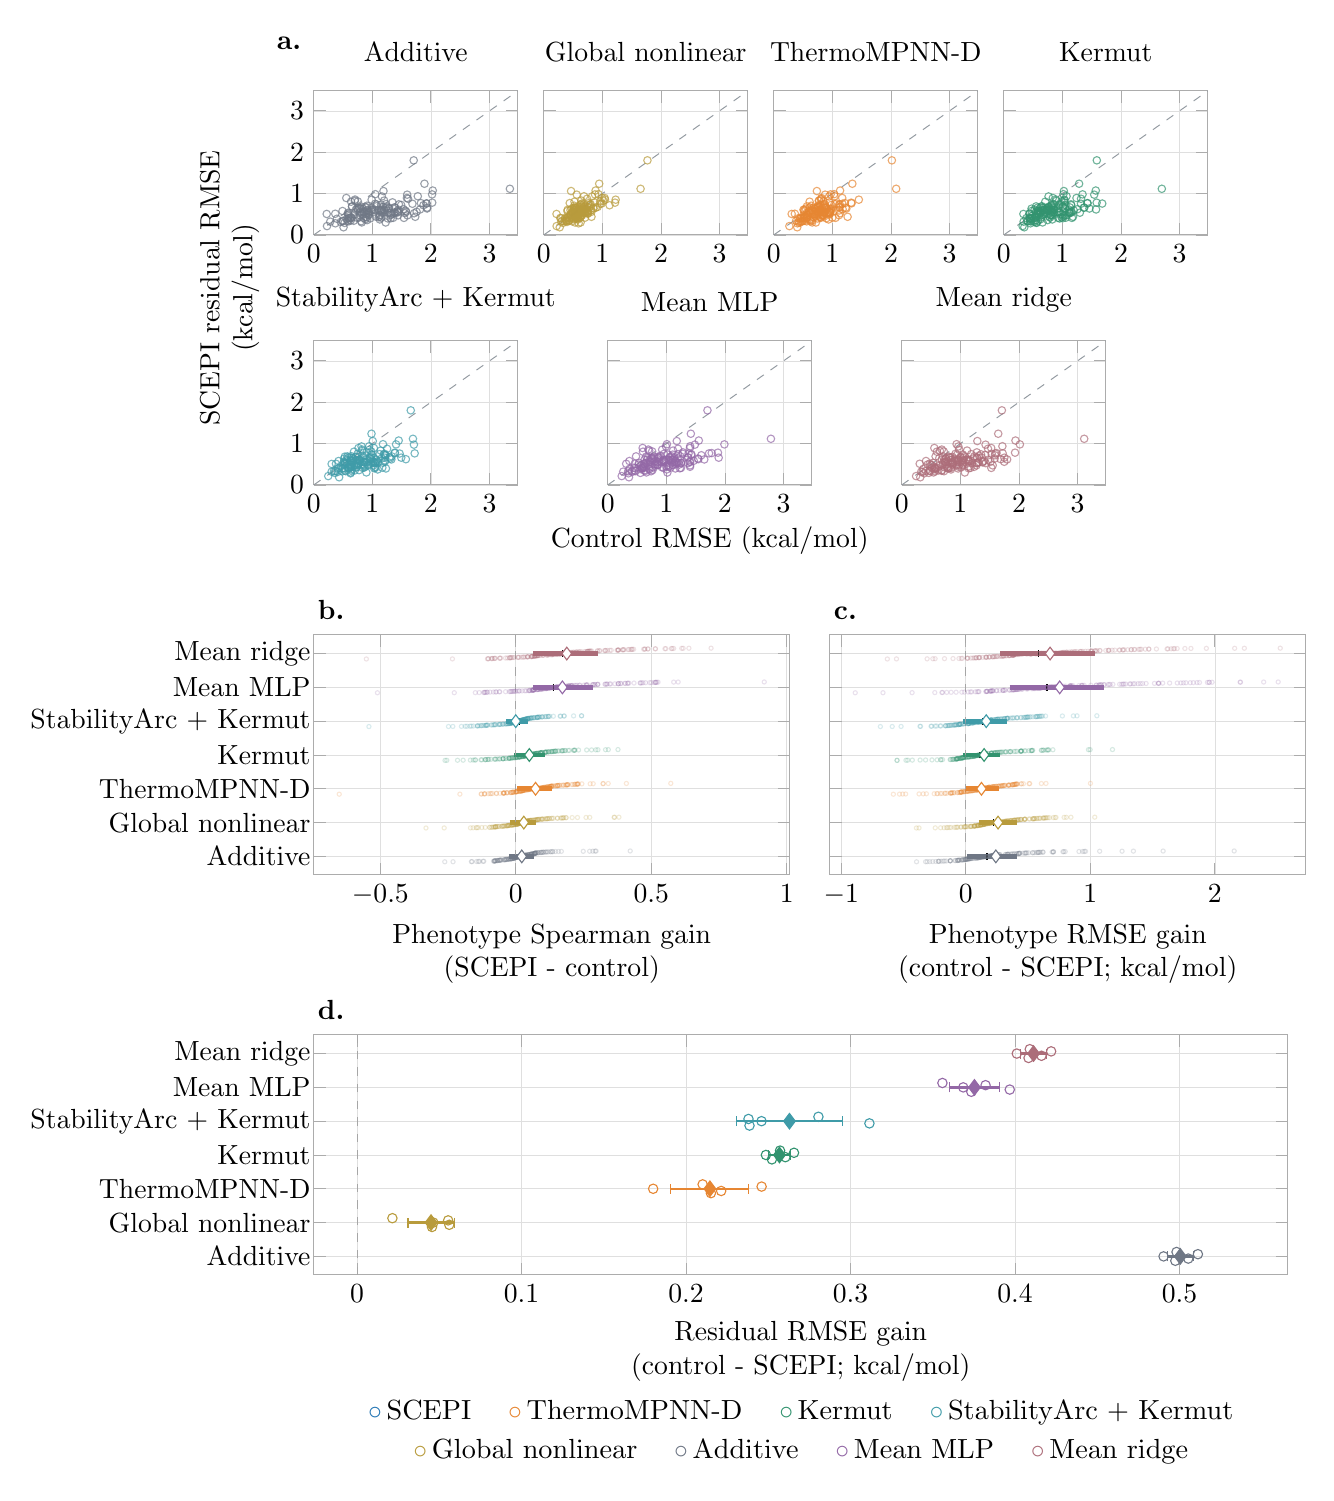
\begin{tikzpicture}[font=\sffamily]
% Self-contained PGFPlots source generated from the verified full-target S-all export.
% The parent manuscript wraps this fragment in a tikzpicture at native size.
\definecolor{predblue}{HTML}{2878B5}
\definecolor{predorange}{HTML}{E68632}
\definecolor{predgreen}{HTML}{32936F}
\definecolor{predteal}{HTML}{3F9BA8}
\definecolor{predgold}{HTML}{B89B3C}
\definecolor{predgray}{HTML}{6F7785}
\definecolor{predpurple}{HTML}{9368A6}
\definecolor{predrose}{HTML}{AC6D79}
\definecolor{preddiag}{HTML}{9299A0}
\begin{groupplot}[
  group style={group name=predtoprowone, group size=4 by 1, horizontal sep=0.13in},
  scale only axis, width=1.02in, height=0.72in, xmin=0, ymin=0,
  xmax=3.481901636, ymax=3.481901636,
  grid=major, grid style={draw=gray!25, line width=0.25pt},
  axis line style={draw=gray!65, line width=0.35pt},
  tick style={draw=gray!65, line width=0.3pt},
  tick label style={font=\normalsize}, label style={font=\normalsize},
  title style={font=\normalsize, yshift=1pt},
]
\nextgroupplot[title={Additive}]
\addplot[only marks, mark=o, mark size=1.35pt, mark options={fill=white}, color=predgray, opacity=0.70] coordinates {(1.1628066637,0.5478488265) (0.7008638006,0.8262331205) (1.4340746459,0.5453556383) (1.7762319142,0.9370040454) (1.0595014981,0.4436593065) (1.1549820867,0.6135008045) (0.7046783491,0.8560432545) (1.1383169246,0.4853682255) (0.2215110595,0.5082911429) (1.0737590192,0.6954799923) (0.6377833988,0.804618651) (0.9646939767,0.4012284104) (0.7493011888,0.6090111844) (1.7559418111,0.5612634826) (1.7063569434,1.8048058015) (1.3541283427,0.4141962736) (1.5323039691,0.6235943884) (1.4418655745,0.5643514921) (1.3066624038,0.52583927) (0.9095499251,0.7075487553) (1.568478433,0.5853323135) (1.2656386972,0.3994164497) (1.4530260243,0.7410623184) (3.3479823423,1.1166104286) (0.6331925985,0.4280839515) (0.8470631037,0.5569190067) (0.7837722664,0.5350809132) (1.0359162966,0.6092270414) (0.7411416521,0.4147232314) (1.2846847495,0.6551101166) (1.4429452464,0.6109087214) (0.9924403279,0.6594113837) (1.5899509181,0.8942509713) (0.226687443,0.2149622621) (0.9332297671,0.5281411994) (0.8484737635,0.4110623019) (1.3126217301,0.4037561263) (0.9367529524,0.5625788946) (1.1110562512,0.4273721696) (0.5875168878,0.407899123) (0.8282295359,0.5030034952) (0.7175220222,0.6102387229) (0.6547082638,0.6916588219) (1.1775959839,0.5466435359) (0.7418824617,0.6492241535) (0.9136983918,0.6004969522) (0.4607052033,0.3149668601) (0.7749685774,0.6362796494) (0.8393561282,0.6329682548) (0.6438392242,0.4085659864) (0.5861048689,0.536775446) (1.1504223387,0.6001500769) (0.8827156406,0.4393127439) (0.9316893848,0.4909958142) (1.1551671866,0.5852679399) (1.2531849478,0.5921357493) (0.5835573205,0.3469081335) (1.6845508836,0.7546195273) (1.6101055028,0.8756709573) (0.526480767,0.2920434567) (0.8993475655,0.6667505376) (1.3759553529,0.54520087) (1.233817173,0.746888189) (0.4911560223,0.5792907785) (1.5950500604,0.9749399244) (2.0223576512,0.7814074893) (0.5960069383,0.3300406351) (0.8590728063,0.5476597743) (1.9283297499,0.7645188029) (0.367405019,0.5129896946) (0.5610813361,0.3861604689) (2.0314933488,1.0745592436) (1.9212804022,0.7596931685) (0.4921092661,0.3413010897) (0.8090180296,0.3328654222) (0.8688781885,0.5502240134) (1.5991901218,0.4734236789) (0.6291577484,0.4190660274) (0.5558332202,0.894213539) (1.5396885037,0.4136783269) (0.6315994271,0.3507987876) (2.0203399605,0.9815739314) (1.2289908913,0.6502015209) (1.1237655793,0.4478133423) (1.9343432293,0.6401703592) (0.9877773508,0.853334288) (1.2407286132,0.6917853192) (0.9048171469,0.4271401092) (1.304809633,0.4773243771) (1.2018412074,0.8319513168) (1.0001850185,0.6162023255) (1.2276601066,0.3022061769) (1.492132524,0.7256757814) (1.2010655751,0.5933708198) (1.0748787637,0.7365427789) (0.7826440539,0.6577294035) (1.3631267574,0.516575917) (0.7902801777,0.5622752283) (0.7879177638,0.4779177953) (1.0505923202,0.9864264805) (0.7991921311,0.6383843765) (1.2816257103,0.6426472002) (1.3849466535,0.661003242) (0.6945970193,0.493972413) (1.7326024769,0.4399729621) (1.8290770108,0.7712603801) (1.1274132269,0.5948282429) (1.3781560817,0.6680084995) (1.0061384396,0.5507805548) (0.9003883458,0.496335552) (0.9140564873,0.5885356615) (0.9494942904,0.579804918) (1.7135058637,0.5258642658) (1.4395797997,0.4745981322) (1.1812811953,0.6768621185) (1.1542829539,0.418389126) (1.2754895129,0.5339254207) (1.3202861959,0.4960109729) (1.393647999,0.5382557492) (0.9390222938,0.4794607811) (0.9792352476,0.5917401421) (1.5555131224,0.5276480472) (1.8719431409,0.7188517767) (1.1483660064,0.733764914) (1.4254833062,0.5699211636) (0.8759459518,0.6780597887) (1.8898689022,1.2391006459) (0.6537828722,0.6861246272) (0.6037137317,0.4568004068) (1.1635917397,0.9316424987) (1.3440611579,0.7886666813) (1.201511634,0.6120483833) (1.0469206235,0.7534562288) (0.911159805,0.3599272856) (0.5012740579,0.3337187762) (0.8179149065,0.6832072207) (1.1055795914,0.6093868258) (0.7714376306,0.4211634684) (0.5829834559,0.5147987886) (1.5773645027,0.5610879331) (1.8145836642,0.6172969729) (1.1903314436,1.0620823257) (1.9353899467,0.6603523384) (0.7529089886,0.8111981887) (0.6078994942,0.4025132735) (0.3962304042,0.3917141594) (0.6829306186,0.3433088627) (0.5085034888,0.1865318263) (0.8828007782,0.3789865754) (1.127278146,0.3759181493) (0.3688592487,0.2824383075) (0.591363819,0.4865240709) (0.8199620362,0.3037412097) (0.281620803,0.3223665106) (1.1242162711,0.4825886046)};
\addplot[no marks, dashed, color=preddiag, line width=0.35pt] coordinates {(0,0) (3.481901636,3.481901636)};
\nextgroupplot[title={Global nonlinear},yticklabels=\empty]
\addplot[only marks, mark=o, mark size=1.35pt, mark options={fill=white}, color=predgold, opacity=0.70] coordinates {(0.5315441109,0.5478488265) (1.0172263349,0.8262331205) (0.4918990451,0.5453556383) (0.6870902264,0.9370040454) (0.4914443733,0.4436593065) (0.6946958479,0.6135008045) (1.0442622607,0.8560432545) (0.537589096,0.4853682255) (0.2182255991,0.5082911429) (0.6131710564,0.6954799923) (0.5250344195,0.804618651) (0.5620663301,0.4012284104) (0.4089645878,0.6090111844) (0.755718387,0.5612634826) (1.7700899148,1.8048058015) (0.5574345621,0.4141962736) (0.7334421966,0.6235943884) (0.6946447937,0.5643514921) (0.599798725,0.52583927) (0.5202957845,0.7075487553) (0.7362504681,0.5853323135) (0.5738282996,0.3994164497) (0.8012877258,0.7410623184) (1.6525547803,1.1166104286) (0.5418480439,0.4280839515) (0.6739418054,0.5569190067) (0.6212932678,0.5350809132) (0.6252234282,0.6092270414) (0.3679643904,0.4147232314) (0.5211797559,0.6551101166) (0.6717945583,0.6109087214) (0.5616873706,0.6594113837) (0.9944463604,0.8942509713) (0.2201019277,0.2149622621) (0.4976209499,0.5281411994) (0.2824026954,0.4110623019) (0.3982235751,0.4037561263) (0.7441301391,0.5625788946) (0.5822451229,0.4273721696) (0.4430909773,0.407899123) (0.501570368,0.5030034952) (0.5229987187,0.6102387229) (0.653375279,0.6916588219) (0.611218486,0.5466435359) (0.6746619905,0.6492241535) (0.613759635,0.6004969522) (0.39607244,0.3149668601) (0.4767953706,0.6362796494) (0.6785691032,0.6329682548) (0.5022157979,0.4085659864) (0.6569315316,0.536775446) (0.4563496189,0.6001500769) (0.4172574581,0.4393127439) (0.4698862588,0.4909958142) (0.5206972068,0.5852679399) (0.680469785,0.5921357493) (0.3917007507,0.3469081335) (0.9636954857,0.7546195273) (0.7389999016,0.8756709573) (0.3279906974,0.2920434567) (0.5422551114,0.6667505376) (0.6824378603,0.54520087) (0.6868099324,0.746888189) (0.4038747689,0.5792907785) (0.5629393571,0.9749399244) (1.2170209684,0.7814074893) (0.4852506747,0.3300406351) (0.6291773469,0.5476597743) (0.7606248377,0.7645188029) (0.4593401104,0.5129896946) (0.36184117,0.3861604689) (0.8849279237,1.0745592436) (0.9876570788,0.7596931685) (0.3130335639,0.3413010897) (0.3567835003,0.3328654222) (0.7081431767,0.5502240134) (0.6537939874,0.4734236789) (0.4299729568,0.4190660274) (1.0397629457,0.894213539) (0.6185185709,0.4136783269) (0.4364012781,0.3507987876) (0.8746878261,0.9815739314) (0.8449273861,0.6502015209) (0.6104170946,0.4478133423) (0.8513427368,0.6401703592) (1.2275990278,0.853334288) (0.697797206,0.6917853192) (0.5904143905,0.4271401092) (0.6464280644,0.4773243771) (0.6425648052,0.8319513168) (0.6109236073,0.6162023255) (0.5340042575,0.3022061769) (0.6317157174,0.7256757814) (0.8056112102,0.5933708198) (0.6270982576,0.7365427789) (0.5179075335,0.6577294035) (0.7529533394,0.516575917) (0.4965921201,0.5622752283) (0.5945901495,0.4779177953) (0.9334103691,0.9864264805) (0.6138703231,0.6383843765) (0.5511886326,0.6426472002) (0.7683022483,0.661003242) (0.5358929857,0.493972413) (0.8147684364,0.4399729621) (0.443816298,0.7712603801) (0.5342306938,0.5948282429) (0.6026911938,0.6680084995) (0.4890630795,0.5507805548) (0.5524235172,0.496335552) (0.6081928058,0.5885356615) (0.6669998017,0.579804918) (0.7560175041,0.5258642658) (0.5666293062,0.4745981322) (0.7450890098,0.6768621185) (0.7046245918,0.418389126) (0.5333229789,0.5339254207) (0.5524937332,0.4960109729) (0.6954227825,0.5382557492) (0.4599646893,0.4794607811) (0.57694874,0.5917401421) (0.7371544075,0.5276480472) (1.1236178609,0.7188517767) (0.7871562555,0.733764914) (0.5427047191,0.5699211636) (0.9192382575,0.6780597887) (0.9468441156,1.2391006459) (0.7992208906,0.6861246272) (0.529850292,0.4568004068) (0.824151091,0.9316424987) (0.8660720285,0.7886666813) (0.629438391,0.6120483833) (0.6409595756,0.7534562288) (0.3822664198,0.3599272856) (0.3863356386,0.3337187762) (0.7165154076,0.6832072207) (0.5331944688,0.6093868258) (0.6244227113,0.4211634684) (0.5690874798,0.5147987886) (0.814146654,0.5610879331) (0.6940865926,0.6172969729) (0.4666706916,1.0620823257) (0.8883400744,0.6603523384) (0.9625468055,0.8111981887) (0.2948276579,0.4025132735) (0.5378288195,0.3917141594) (0.4291568042,0.3433088627) (0.2729877924,0.1865318263) (0.5166411822,0.3789865754) (0.5828465871,0.3759181493) (0.596184405,0.2824383075) (0.5932681219,0.4865240709) (0.6295902228,0.3037412097) (0.2993852518,0.3223665106) (0.6439835054,0.4825886046)};
\addplot[no marks, dashed, color=preddiag, line width=0.35pt] coordinates {(0,0) (3.481901636,3.481901636)};
\nextgroupplot[title={ThermoMPNN-D},yticklabels=\empty]
\addplot[only marks, mark=o, mark size=1.35pt, mark options={fill=white}, color=predorange, opacity=0.70] coordinates {(0.9568483718,0.5478488265) (0.7685519886,0.8262331205) (0.8448775896,0.5453556383) (1.0376133045,0.9370040454) (0.7980784872,0.4436593065) (0.9741025507,0.6135008045) (0.8106492606,0.8560432545) (0.7670722028,0.4853682255) (0.3060622978,0.5082911429) (0.7578497369,0.6954799923) (0.6122553227,0.804618651) (0.5554128482,0.4012284104) (0.5212000693,0.6090111844) (0.8695614575,0.5612634826) (2.0163960963,1.8048058015) (1.0540643054,0.4141962736) (1.1761144704,0.6235943884) (0.7653711071,0.5643514921) (0.7538530254,0.52583927) (0.6389079152,0.7075487553) (0.7832041583,0.5853323135) (0.7480956053,0.3994164497) (1.1250143826,0.7410623184) (2.0897117914,1.1166104286) (0.6782165728,0.4280839515) (0.8041882183,0.5569190067) (0.5962787549,0.5350809132) (0.7852257193,0.6092270414) (0.5058235016,0.4147232314) (0.8780539626,0.6551101166) (0.8307366037,0.6109087214) (0.7215021969,0.6594113837) (1.1691424013,0.8942509713) (0.2669351803,0.2149622621) (0.5677812822,0.5281411994) (0.4816110399,0.4110623019) (0.8958237456,0.4037561263) (0.8535074659,0.5625788946) (0.6836769361,0.4273721696) (0.4587400806,0.407899123) (0.6984871963,0.5030034952) (0.5073567578,0.6102387229) (0.5662322679,0.6916588219) (0.9537822528,0.5466435359) (0.9041372946,0.6492241535) (0.6500589543,0.6004969522) (0.461373799,0.3149668601) (0.5467576221,0.6362796494) (0.7070698884,0.6329682548) (0.5699493387,0.4085659864) (0.6396350754,0.536775446) (0.6407630339,0.6001500769) (0.5737176908,0.4393127439) (0.8282406745,0.4909958142) (0.9766522152,0.5852679399) (0.9572942353,0.5921357493) (0.3823828813,0.3469081335) (1.1718907923,0.7546195273) (0.8078223144,0.8756709573) (0.436212131,0.2920434567) (0.6141877374,0.6667505376) (0.9557339198,0.54520087) (1.037888958,0.746888189) (0.524796881,0.5792907785) (0.8766771438,0.9749399244) (1.3219410665,0.7814074893) (0.5614967418,0.3300406351) (0.8269469715,0.5476597743) (1.3278030067,0.7645188029) (0.3602260292,0.5129896946) (0.518002544,0.3861604689) (1.1324672023,1.0745592436) (1.0724470526,0.7596931685) (0.4976742587,0.3413010897) (0.6309167086,0.3328654222) (0.6679839045,0.5502240134) (0.8373069774,0.4734236789) (0.5365508404,0.4190660274) (0.8152471449,0.894213539) (0.8009825782,0.4136783269) (0.6535533131,0.3507987876) (0.9699945722,0.9815739314) (0.8265527332,0.6502015209) (0.8596560729,0.4478133423) (1.2399522782,0.6401703592) (1.45247472,0.853334288) (0.8666883608,0.6917853192) (0.8011279391,0.4271401092) (1.1136500835,0.4773243771) (0.7767026636,0.8319513168) (0.7894374525,0.6162023255) (0.7201605318,0.3022061769) (0.9802946043,0.7256757814) (1.1162702961,0.5933708198) (0.7930086833,0.7365427789) (0.6824250025,0.6577294035) (0.9600644344,0.516575917) (0.6034858496,0.5622752283) (0.8515649772,0.4779177953) (1.0292906481,0.9864264805) (0.9730506003,0.6383843765) (0.6972868505,0.6426472002) (0.8529434536,0.661003242) (0.7457396273,0.493972413) (1.2607907064,0.4399729621) (1.2144261763,0.7712603801) (0.6005810529,0.5948282429) (1.1135333571,0.6680084995) (0.8021688984,0.5507805548) (0.6652363396,0.496335552) (0.7313415161,0.5885356615) (0.6579666347,0.579804918) (1.132121772,0.5258642658) (0.8213322205,0.4745981322) (1.1264998799,0.6768621185) (1.0003364443,0.418389126) (0.8617254955,0.5339254207) (0.9339855184,0.4960109729) (0.9057417479,0.5382557492) (0.5049319716,0.4794607811) (0.8099011028,0.5917401421) (0.9300951165,0.5276480472) (1.1126667796,0.7188517767) (0.8713874899,0.733764914) (0.7727217069,0.5699211636) (0.7691993129,0.6780597887) (1.3414808337,1.2391006459) (0.7514374313,0.6861246272) (0.5215446152,0.4568004068) (0.9443916707,0.9316424987) (0.9496007368,0.7886666813) (0.7672381516,0.6120483833) (0.8532780491,0.7534562288) (0.6241027633,0.3599272856) (0.4835358019,0.3337187762) (0.8863582979,0.6832072207) (0.7870660164,0.6093868258) (0.5648530312,0.4211634684) (0.7190643776,0.5147987886) (0.9597671843,0.5610879331) (0.9043813262,0.6172969729) (0.736480765,1.0620823257) (1.2266270869,0.6603523384) (0.8476129708,0.8111981887) (0.4193283252,0.4025132735) (0.4481687919,0.3917141594) (0.5274535583,0.3433088627) (0.4012788364,0.1865318263) (0.6087130043,0.3789865754) (0.9348423202,0.3759181493) (0.404734975,0.2824383075) (0.5828077192,0.4865240709) (0.655644918,0.3037412097) (0.4247625068,0.3223665106) (0.7300308969,0.4825886046)};
\addplot[no marks, dashed, color=preddiag, line width=0.35pt] coordinates {(0,0) (3.481901636,3.481901636)};
\nextgroupplot[title={Kermut},yticklabels=\empty]
\addplot[only marks, mark=o, mark size=1.35pt, mark options={fill=white}, color=predgreen, opacity=0.70] coordinates {(0.8579191276,0.5478488265) (0.8970689066,0.8262331205) (0.948513695,0.5453556383) (1.0717554458,0.9370040454) (0.7778177441,0.4436593065) (0.859947777,0.6135008045) (0.8895988081,0.8560432545) (0.8027259609,0.4853682255) (0.3352512474,0.5082911429) (0.6523344078,0.6954799923) (0.7088231198,0.804618651) (0.4480261755,0.4012284104) (0.686485844,0.6090111844) (0.8250908697,0.5612634826) (1.5884504305,1.8048058015) (0.9267091101,0.4141962736) (1.2587318663,0.6235943884) (0.5841455712,0.5643514921) (0.5829454457,0.52583927) (0.8155062606,0.7075487553) (0.6243397317,0.5853323135) (0.9531129036,0.3994164497) (1.1471117277,0.7410623184) (2.6979703626,1.1166104286) (0.5527254192,0.4280839515) (0.6962911966,0.5569190067) (0.6304082319,0.5350809132) (0.8251311095,0.6092270414) (0.525762648,0.4147232314) (0.8480216162,0.6551101166) (0.7572965025,0.6109087214) (0.5771659649,0.6594113837) (1.2414379435,0.8942509713) (0.3214715095,0.2149622621) (0.5833231136,0.5281411994) (0.4806542186,0.4110623019) (1.0061094538,0.4037561263) (1.0225012508,0.5625788946) (0.9858636041,0.4273721696) (0.3866231688,0.407899123) (0.6911071152,0.5030034952) (0.5262454171,0.6102387229) (0.551841322,0.6916588219) (1.1121336715,0.5466435359) (0.618735549,0.6492241535) (0.8469239624,0.6004969522) (0.5258811868,0.3149668601) (0.4740694914,0.6362796494) (0.7952777699,0.6329682548) (0.4569559491,0.4085659864) (0.5494733435,0.536775446) (0.653706663,0.6001500769) (0.5487392321,0.4393127439) (0.6690439074,0.4909958142) (0.5908416724,0.5852679399) (0.7790814277,0.5921357493) (0.5118827283,0.3469081335) (1.3188494301,0.7546195273) (1.3188442056,0.8756709573) (0.5593531358,0.2920434567) (0.7714682412,0.6667505376) (1.1275130745,0.54520087) (0.9764647855,0.746888189) (0.4749050531,0.5792907785) (1.5439541839,0.9749399244) (1.5856524035,0.7814074893) (0.4657152453,0.3300406351) (0.6321413043,0.5476597743) (1.4266102244,0.7645188029) (0.4406286816,0.5129896946) (0.463385323,0.3861604689) (1.5709373976,1.0745592436) (1.6808373105,0.7596931685) (0.4038667684,0.3413010897) (0.4572695008,0.3328654222) (0.8168894045,0.5502240134) (0.8330703742,0.4734236789) (0.5486423731,0.4190660274) (0.8372637952,0.894213539) (1.1638437075,0.4136783269) (0.5394049038,0.3507987876) (1.3451548646,0.9815739314) (1.0404528708,0.6502015209) (1.0144197281,0.4478133423) (1.4618388932,0.6401703592) (1.0362590794,0.853334288) (1.0099330244,0.6917853192) (0.6446206432,0.4271401092) (1.0766931518,0.4773243771) (1.0325323504,0.8319513168) (0.8666908328,0.6162023255) (0.5584612927,0.3022061769) (1.0536980518,0.7256757814) (1.1942760491,0.5933708198) (0.9478956138,0.7365427789) (0.6700062676,0.6577294035) (0.8387490028,0.516575917) (0.623847752,0.5622752283) (0.6468978147,0.4779177953) (1.018748661,0.9864264805) (0.7339275353,0.6383843765) (0.9201988039,0.6426472002) (1.3752818136,0.661003242) (0.5712665808,0.493972413) (1.1821072854,0.4399729621) (1.4303299155,0.7712603801) (0.760553959,0.5948282429) (1.126714339,0.6680084995) (0.9210725045,0.5507805548) (0.9714431603,0.496335552) (0.6756416954,0.5885356615) (0.5575179294,0.579804918) (0.7132472938,0.5258642658) (1.0397404718,0.4745981322) (1.0038134163,0.6768621185) (1.0593838495,0.418389126) (1.1425528508,0.5339254207) (1.0011317377,0.4960109729) (1.2992814673,0.5382557492) (0.7959488758,0.4794607811) (0.7356558558,0.5917401421) (1.1190805293,0.5276480472) (1.1513843726,0.7188517767) (0.8559195124,0.733764914) (0.7964300895,0.5699211636) (0.8140836629,0.6780597887) (1.286208639,1.2391006459) (0.6384706214,0.6861246272) (0.4759677561,0.4568004068) (0.7646344949,0.9316424987) (1.033773592,0.7886666813) (1.1140983963,0.6120483833) (0.8340767185,0.7534562288) (0.7493974363,0.3599272856) (0.4128768736,0.3337187762) (0.7637759162,0.6832072207) (0.6966554867,0.6093868258) (0.7905193837,0.4211634684) (0.4362546621,0.5147987886) (1.1586811517,0.5610879331) (1.5758745344,0.6172969729) (1.0263907123,1.0620823257) (1.3661093261,0.6603523384) (0.9839862399,0.8111981887) (0.4405479861,0.4025132735) (0.4405059088,0.3917141594) (0.584854641,0.3433088627) (0.3505113656,0.1865318263) (0.6269060441,0.3789865754) (0.8280802945,0.3759181493) (0.4555332326,0.2824383075) (0.6041967125,0.4865240709) (0.6625571024,0.3037412097) (0.33878183,0.3223665106) (0.8046019231,0.4825886046)};
\addplot[no marks, dashed, color=preddiag, line width=0.35pt] coordinates {(0,0) (3.481901636,3.481901636)};
\end{groupplot}
\begin{scope}[yshift=-1.25in]
\begin{groupplot}[
  group style={group name=predtoprowtwo, group size=3 by 1, horizontal sep=0.45in},
  scale only axis, width=1.02in, height=0.72in, xmin=0, ymin=0,
  xmax=3.481901636, ymax=3.481901636,
  grid=major, grid style={draw=gray!25, line width=0.25pt},
  axis line style={draw=gray!65, line width=0.35pt},
  tick style={draw=gray!65, line width=0.3pt},
  tick label style={font=\normalsize}, label style={font=\normalsize},
  title style={font=\normalsize, yshift=1pt},
]
\nextgroupplot[title={StabilityArc + Kermut}]
\addplot[only marks, mark=o, mark size=1.35pt, mark options={fill=white}, color=predteal, opacity=0.70] coordinates {(1.0136426323,0.5478488265) (0.8290695747,0.8262331205) (0.8686113673,0.5453556383) (0.9459939418,0.9370040454) (0.8789479333,0.4436593065) (0.766946855,0.6135008045) (0.8265723728,0.8560432545) (0.8637289531,0.4853682255) (0.3056530527,0.5082911429) (0.6412431903,0.6954799923) (0.6865711974,0.804618651) (0.5338294733,0.4012284104) (0.7875528714,0.6090111844) (1.0236016931,0.5612634826) (1.655939242,1.8048058015) (1.0477752198,0.4141962736) (1.5730589785,0.6235943884) (0.5163268133,0.5643514921) (0.7574125045,0.52583927) (0.8376252179,0.7075487553) (0.7813644602,0.5853323135) (1.2325207149,0.3994164497) (1.195487378,0.7410623184) (1.693357692,1.1166104286) (0.6353978906,0.4280839515) (0.8526728956,0.5569190067) (0.5349160046,0.5350809132) (0.8925402633,0.6092270414) (0.5864136827,0.4147232314) (0.9606020854,0.6551101166) (0.7814620592,0.6109087214) (0.5887235726,0.6594113837) (1.0260974225,0.8942509713) (0.2476850542,0.2149622621) (0.5629465704,0.5281411994) (0.5851771704,0.4110623019) (1.0316469111,0.4037561263) (0.982302793,0.5625788946) (0.7268097059,0.4273721696) (0.4955406949,0.407899123) (0.7641913674,0.5030034952) (0.5631246657,0.6102387229) (0.5742611348,0.6916588219) (1.0937217395,0.5466435359) (0.6664046025,0.6492241535) (0.7405852313,0.6004969522) (0.408829058,0.3149668601) (0.5188241212,0.6362796494) (0.8048951853,0.6329682548) (0.4233593555,0.4085659864) (0.5122549463,0.536775446) (0.7155470815,0.6001500769) (0.6280549749,0.4393127439) (0.6319417169,0.4909958142) (0.64148429,0.5852679399) (0.7781725086,0.5921357493) (0.5329678088,0.3469081335) (1.2074332567,0.7546195273) (1.252175934,0.8756709573) (0.3614361744,0.2920434567) (0.8459062919,0.6667505376) (1.056435365,0.54520087) (1.1232610483,0.746888189) (0.4238991548,0.5792907785) (1.7100998668,0.9749399244) (1.3825422928,0.7814074893) (0.4873664488,0.3300406351) (0.6225071608,0.5476597743) (1.7228427671,0.7645188029) (0.3792767501,0.5129896946) (0.4834038488,0.3861604689) (1.4502363618,1.0745592436) (1.4661672372,0.7596931685) (0.3724662436,0.3413010897) (0.5479543344,0.3328654222) (0.853827081,0.5502240134) (0.7381828002,0.4734236789) (0.6030393871,0.4190660274) (0.7648828101,0.894213539) (0.8353948748,0.4136783269) (0.7001818553,0.3507987876) (1.404928268,0.9815739314) (1.0289250704,0.6502015209) (0.6539367184,0.4478133423) (1.3068832082,0.6401703592) (0.9513535009,0.853334288) (1.3302772055,0.6917853192) (0.7293560999,0.4271401092) (0.9242888985,0.4773243771) (1.1432155239,0.8319513168) (0.9742701364,0.6162023255) (0.6314489532,0.3022061769) (1.2157579017,0.7256757814) (1.217215098,0.5933708198) (0.9940876598,0.7365427789) (0.6484586052,0.6577294035) (0.7410253562,0.516575917) (0.7406386042,0.5622752283) (0.7228803064,0.4779177953) (1.181947157,0.9864264805) (0.9601672514,0.6383843765) (1.1591471878,0.6426472002) (1.211874096,0.661003242) (0.5989227211,0.493972413) (1.0492662132,0.4399729621) (1.3855534634,0.7712603801) (0.6361984269,0.5948282429) (1.2915556784,0.6680084995) (0.9018438694,0.5507805548) (0.844084216,0.496335552) (0.644594352,0.5885356615) (0.5719003625,0.579804918) (1.0427420529,0.5258642658) (1.0222982567,0.4745981322) (0.9734980492,0.6768621185) (1.1709632919,0.418389126) (1.0434510626,0.5339254207) (0.9331963746,0.4960109729) (1.1805569802,0.5382557492) (0.6916259515,0.4794607811) (0.7170407844,0.5917401421) (1.0060293751,0.5276480472) (1.2275835548,0.7188517767) (0.9803617645,0.733764914) (1.0795594453,0.5699211636) (0.7178819618,0.6780597887) (0.9858908226,1.2391006459) (0.5318028478,0.6861246272) (0.460843262,0.4568004068) (0.8160144375,0.9316424987) (0.9031640927,0.7886666813) (1.0703512286,0.6120483833) (0.7485287982,0.7534562288) (0.7749555371,0.3599272856) (0.3458141957,0.3337187762) (0.721082764,0.6832072207) (0.6619191006,0.6093868258) (0.8615004497,0.4211634684) (0.5269606354,0.5147987886) (1.2142263077,0.5610879331) (1.3254223366,0.6172969729) (1.007658551,1.0620823257) (1.4938558784,0.6603523384) (0.981355813,0.8111981887) (0.6045164711,0.4025132735) (0.4109115606,0.3917141594) (0.6459694352,0.3433088627) (0.4340121891,0.1865318263) (0.6423943706,0.3789865754) (1.0923536445,0.3759181493) (0.6285072729,0.2824383075) (0.6356426923,0.4865240709) (0.8986410328,0.3037412097) (0.3057719087,0.3223665106) (0.8086992791,0.4825886046)};
\addplot[no marks, dashed, color=preddiag, line width=0.35pt] coordinates {(0,0) (3.481901636,3.481901636)};
\nextgroupplot[title={Mean MLP},yticklabels=\empty]
\addplot[only marks, mark=o, mark size=1.35pt, mark options={fill=white}, color=predpurple, opacity=0.70] coordinates {(0.9645219646,0.5478488265) (0.7086067929,0.8262331205) (1.1577077344,0.5453556383) (1.4063098841,0.9370040454) (1.0418838695,0.4436593065) (1.1185236273,0.6135008045) (0.693436552,0.8560432545) (1.1061328982,0.4853682255) (0.6153847771,0.5082911429) (1.0896381664,0.6954799923) (0.6017000257,0.804618651) (0.6977355824,0.4012284104) (0.67259786,0.6090111844) (1.408240837,0.5612634826) (1.7020428821,1.8048058015) (0.9530078091,0.4141962736) (1.5467180053,0.6235943884) (0.9544672734,0.5643514921) (1.2526849052,0.52583927) (0.8998406966,0.7075487553) (1.4682031735,0.5853323135) (1.1532132011,0.3994164497) (1.428171625,0.7410623184) (2.7852771126,1.1166104286) (0.6245258931,0.4280839515) (0.7988696854,0.5569190067) (0.6572131524,0.5350809132) (0.9540954296,0.6092270414) (0.6089534436,0.4147232314) (1.0660672155,0.6551101166) (1.2350565066,0.6109087214) (0.860726402,0.6594113837) (1.4028090381,0.8942509713) (0.2384924262,0.2149622621) (0.6316327219,0.5281411994) (0.5910265829,0.4110623019) (1.2302786522,0.4037561263) (0.8420938046,0.5625788946) (0.9263395754,0.4273721696) (0.5856754961,0.407899123) (0.8121205367,0.5030034952) (0.627843735,0.6102387229) (0.4830015454,0.6916588219) (1.095891708,0.5466435359) (0.6825052503,0.6492241535) (0.7608795192,0.6004969522) (0.4150102514,0.3149668601) (0.7633345967,0.6362796494) (0.8459467483,0.6329682548) (0.4670456617,0.4085659864) (0.5345135354,0.536775446) (0.7118263363,0.6001500769) (0.7607378249,0.4393127439) (0.845806933,0.4909958142) (1.1469930524,0.5852679399) (1.0482622745,0.5921357493) (0.4594287784,0.3469081335) (1.2789729986,0.7546195273) (1.1997554964,0.8756709573) (0.5575272046,0.2920434567) (0.8884909584,0.6667505376) (1.1738071037,0.54520087) (1.2006798456,0.746888189) (0.3692886145,0.5792907785) (1.4871842193,0.9749399244) (1.8810374525,0.7814074893) (0.3478844455,0.3300406351) (0.7225861031,0.5476597743) (1.7293615784,0.7645188029) (0.314724098,0.5129896946) (0.5527946842,0.3861604689) (1.5544573846,1.0745592436) (1.3788304473,0.7596931685) (0.4164535281,0.3413010897) (0.7392811274,0.3328654222) (0.8750101412,0.5502240134) (1.4047391194,0.4734236789) (0.448581116,0.4190660274) (0.5956785508,0.894213539) (1.2501153433,0.4136783269) (0.619947849,0.3507987876) (1.9910446944,0.9815739314) (1.1366083224,0.6502015209) (0.9977318601,0.4478133423) (1.5398123653,0.6401703592) (0.9291329649,0.853334288) (1.241035809,0.6917853192) (0.6142460163,0.4271401092) (1.1149138928,0.4773243771) (1.1151855285,0.8319513168) (1.0004411859,0.6162023255) (1.0181546607,0.3022061769) (1.4228423913,0.7256757814) (1.1056726976,0.5933708198) (1.0247228118,0.7365427789) (0.7564347216,0.6577294035) (1.1358513276,0.516575917) (0.7205200613,0.5622752283) (0.6403245194,0.4779177953) (1.0099802671,0.9864264805) (0.7419208925,0.6383843765) (1.1927360133,0.6426472002) (1.3664367212,0.661003242) (0.5274322642,0.493972413) (1.4044465916,0.4399729621) (1.7745867355,0.7712603801) (0.9577312554,0.5948282429) (1.3756210021,0.6680084995) (0.920428911,0.5507805548) (0.8070888373,0.496335552) (0.8792454964,0.5885356615) (0.8095686198,0.579804918) (1.1777867277,0.5258642658) (1.0116028007,0.4745981322) (1.0599109888,0.6768621185) (1.0704127427,0.418389126) (1.2516036047,0.5339254207) (1.2231964472,0.4960109729) (1.2082565319,0.5382557492) (0.8471069518,0.4794607811) (0.9675242853,0.5917401421) (1.3709103203,0.5276480472) (1.5976537697,0.7188517767) (1.1089135141,0.733764914) (0.9606709896,0.5699211636) (0.857273756,0.6780597887) (1.4183026253,1.2391006459) (0.6564795745,0.6861246272) (0.600973318,0.4568004068) (0.9936268321,0.9316424987) (1.2831354751,0.7886666813) (1.0948286406,0.6120483833) (0.9600646689,0.7534562288) (0.7642683158,0.3599272856) (0.4767437012,0.3337187762) (0.7919353586,0.6832072207) (1.0418300005,0.6093868258) (0.7740953934,0.4211634684) (0.4605984331,0.5147987886) (1.3968726536,0.5610879331) (1.647926194,0.6172969729) (1.1786651994,1.0620823257) (1.8936182693,0.6603523384) (0.7584632038,0.8111981887) (0.5828847527,0.4025132735) (0.3737393983,0.3917141594) (0.6448714758,0.3433088627) (0.3628408425,0.1865318263) (0.7107830948,0.3789865754) (1.0076399584,0.3759181493) (0.3524580181,0.2824383075) (0.5723083372,0.4865240709) (0.6597673114,0.3037412097) (0.2646235298,0.3223665106) (0.8600666194,0.4825886046)};
\addplot[no marks, dashed, color=preddiag, line width=0.35pt] coordinates {(0,0) (3.481901636,3.481901636)};
\nextgroupplot[title={Mean ridge},yticklabels=\empty]
\addplot[only marks, mark=o, mark size=1.35pt, mark options={fill=white}, color=predrose, opacity=0.70] coordinates {(0.8737350718,0.5478488265) (0.6504511716,0.8262331205) (1.3793087434,0.5453556383) (1.71790006,0.9370040454) (0.9669136933,0.4436593065) (1.1442218225,0.6135008045) (0.6839412448,0.8560432545) (0.9806703965,0.4853682255) (0.8772533154,0.5082911429) (1.0722345159,0.6954799923) (0.5997118606,0.804618651) (0.7929704141,0.4012284104) (0.685761457,0.6090111844) (1.7499171807,0.5612634826) (1.7091676111,1.8048058015) (1.1746085916,0.4141962736) (1.6894329834,0.6235943884) (1.3845376704,0.5643514921) (1.2002434844,0.52583927) (1.3191289759,0.7075487553) (1.4078751943,0.5853323135) (0.9623104657,0.3994164497) (1.3529909767,0.7410623184) (3.1141058458,1.1166104286) (0.5590739078,0.4280839515) (0.7370927762,0.5569190067) (0.707141805,0.5350809132) (0.9663719988,0.6092270414) (0.60288419,0.4147232314) (1.2895465748,0.6551101166) (1.473754959,0.6109087214) (1.0018385017,0.6594113837) (1.5268243398,0.8942509713) (0.2449172159,0.2149622621) (0.8407527146,0.5281411994) (0.8395786078,0.4110623019) (1.1422688689,0.4037561263) (0.7877926562,0.5625788946) (1.017141861,0.4273721696) (0.5694010402,0.407899123) (0.7614990652,0.5030034952) (0.7273207578,0.6102387229) (0.5774982424,0.6916588219) (1.0437076865,0.5466435359) (0.6406052156,0.6492241535) (0.8354352246,0.6004969522) (0.3564032065,0.3149668601) (0.7511087087,0.6362796494) (0.9023293151,0.6329682548) (0.5722152365,0.4085659864) (0.5359611756,0.536775446) (0.8399484616,0.6001500769) (0.7828585477,0.4393127439) (0.8616849457,0.4909958142) (1.141003521,0.5852679399) (1.0336197194,0.5921357493) (0.4735760655,0.3469081335) (1.5347561238,0.7546195273) (1.4721995415,0.8756709573) (0.4621244974,0.2920434567) (0.8277915535,0.6667505376) (1.311715692,0.54520087) (1.1867930874,0.746888189) (0.4140915183,0.5792907785) (1.4307466126,0.9749399244) (1.9341863503,0.7814074893) (0.5654148094,0.3300406351) (0.7487058024,0.5476597743) (1.7227502634,0.7645188029) (0.3066642637,0.5129896946) (0.5792399054,0.3861604689) (1.9410899797,1.0745592436) (1.597681918,0.7596931685) (0.4100637646,0.3413010897) (0.7210785019,0.3328654222) (0.8599041162,0.5502240134) (1.5524550157,0.4734236789) (0.5118853423,0.4190660274) (0.5561002904,0.894213539) (1.5287007312,0.4136783269) (0.625672374,0.3507987876) (2.0166068975,0.9815739314) (1.0547777084,0.6502015209) (1.1440657329,0.4478133423) (1.5861923491,0.6401703592) (0.9816189959,0.853334288) (1.2382202877,0.6917853192) (0.7308679876,0.4271401092) (1.0371547325,0.4773243771) (1.115123353,0.8319513168) (0.957698684,0.6162023255) (1.0766865776,0.3022061769) (1.4274020611,0.7256757814) (1.0504294394,0.5933708198) (1.0412861971,0.7365427789) (0.8049201717,0.6577294035) (1.1092923812,0.516575917) (0.7463286941,0.5622752283) (0.5187915893,0.4779177953) (0.9361879567,0.9864264805) (0.7554790069,0.6383843765) (1.2227981491,0.6426472002) (1.3673248323,0.661003242) (0.4410933422,0.493972413) (1.2374165014,0.4399729621) (1.6176382314,0.7712603801) (1.058896285,0.5948282429) (1.2796290879,0.6680084995) (0.9780012612,0.5507805548) (0.9342811483,0.496335552) (0.9625792429,0.5885356615) (0.9009082071,0.579804918) (1.2797369219,0.5258642658) (1.2747736905,0.4745981322) (1.0042037033,0.6768621185) (0.8182446677,0.418389126) (1.2724449985,0.5339254207) (1.0426444944,0.4960109729) (1.2936194639,0.5382557492) (0.9469910316,0.4794607811) (0.9269681274,0.5917401421) (1.4323109685,0.5276480472) (1.5899607199,0.7188517767) (0.9462334928,0.733764914) (1.1418184634,0.5699211636) (0.8660508061,0.6780597887) (1.6468779388,1.2391006459) (0.7051517749,0.6861246272) (0.6328652712,0.4568004068) (0.9664632002,0.9316424987) (1.2812901942,0.7886666813) (1.1233197871,0.6120483833) (0.9167479987,0.7534562288) (0.6840092911,0.3599272856) (0.4829924157,0.3337187762) (0.8065030749,0.6832072207) (1.0948477393,0.6093868258) (0.7668749531,0.4211634684) (0.4778818204,0.5147987886) (1.5150527604,0.5610879331) (1.799017258,0.6172969729) (1.2904382542,1.0620823257) (1.7510787716,0.6603523384) (0.7170597806,0.8111981887) (0.7896253408,0.4025132735) (0.3711468745,0.3917141594) (0.6812490798,0.3433088627) (0.3161400776,0.1865318263) (0.5517517888,0.3789865754) (0.8409718103,0.3759181493) (0.3825881217,0.2824383075) (0.6992090071,0.4865240709) (0.5430487516,0.3037412097) (0.3332004499,0.3223665106) (0.4985758491,0.4825886046)};
\addplot[no marks, dashed, color=preddiag, line width=0.35pt] coordinates {(0,0) (3.481901636,3.481901636)};
\end{groupplot}
\end{scope}
\node[anchor=south east, xshift=-1pt, yshift=0.16in, font=\bfseries\normalsize] at (predtoprowone c1r1.north west) {a.};
\node[rotate=90, align=center, font=\normalsize] at ($(predtoprowone c1r1.west)!0.5!(predtoprowtwo c1r1.west)+(-0.42in,0)$) {SCEPI residual RMSE\\(kcal/mol)};
\node[align=center, font=\normalsize] at ($(predtoprowtwo c1r1.south)!0.5!(predtoprowtwo c3r1.south)+(0,-0.28in)$) {Control RMSE (kcal/mol)};
\begin{scope}[yshift=-3.20in]
\begin{groupplot}[
  group style={group name=predlower, group size=2 by 1, horizontal sep=0.20in},
  scale only axis, width=2.38in, height=1.20in, ymin=-0.55, ymax=6.55,
  ytick={0,1,2,3,4,5,6}, yticklabels={Additive,Global nonlinear,ThermoMPNN-D,Kermut,StabilityArc + Kermut,Mean MLP,Mean ridge},
  grid=major, grid style={draw=gray!25, line width=0.25pt},
  axis line style={draw=gray!65, line width=0.35pt}, tick style={draw=gray!65, line width=0.3pt},
  tick label style={font=\normalsize}, label style={font=\normalsize},
  yticklabel style={font=\normalsize, inner xsep=1pt}, xlabel style={font=\normalsize, align=center},
]
\nextgroupplot[xmin=-0.7460245336,xmax=1.0111344724,xlabel={Phenotype Spearman gain\\(SCEPI - control)}]
\addplot[only marks, mark=o, mark size=0.75pt, mark options={fill=predgray!25}, color=predgray, opacity=0.20] coordinates {(-0.262254574,-0.16) (-0.2317290984,-0.1579746835) (-0.1640468954,-0.1559493671) (-0.161644899,-0.1539240506) (-0.1447050091,-0.1518987342) (-0.1381150278,-0.1498734177) (-0.1344326004,-0.1478481013) (-0.1210621389,-0.1458227848) (-0.1181724653,-0.1437974684) (-0.0824318103,-0.1417721519) (-0.0796837648,-0.1397468354) (-0.0792823549,-0.137721519) (-0.0789800177,-0.1356962025) (-0.0773228466,-0.1336708861) (-0.0763342692,-0.1316455696) (-0.0749898647,-0.1296202532) (-0.0731884514,-0.1275949367) (-0.0688942656,-0.1255696203) (-0.0683352195,-0.1235443038) (-0.0674250894,-0.1215189873) (-0.0643706294,-0.1194936709) (-0.061228727,-0.1174683544) (-0.0611573566,-0.115443038) (-0.0582967033,-0.1134177215) (-0.0580657915,-0.1113924051) (-0.0576843446,-0.1093670886) (-0.0539325986,-0.1073417722) (-0.0530804143,-0.1053164557) (-0.045381905,-0.1032911392) (-0.0421769358,-0.1012658228) (-0.0417567102,-0.0992405063) (-0.039826806,-0.0972151899) (-0.0381167415,-0.0951898734) (-0.0357052783,-0.093164557) (-0.0355291309,-0.0911392405) (-0.0338434538,-0.0891139241) (-0.0323870012,-0.0870886076) (-0.0270399485,-0.0850632911) (-0.0269764942,-0.0830379747) (-0.0257344938,-0.0810126582) (-0.0250688108,-0.0789873418) (-0.0202426112,-0.0769620253) (-0.0197120527,-0.0749367089) (-0.0189636777,-0.0729113924) (-0.0183270154,-0.0708860759) (-0.0158176646,-0.0688607595) (-0.0154493246,-0.066835443) (-0.0154052115,-0.0648101266) (-0.0126984912,-0.0627848101) (-0.0121953386,-0.0607594937) (-0.0096534902,-0.0587341772) (-0.0092125509,-0.0567088608) (-0.0089479375,-0.0546835443) (-0.0087586183,-0.0526582278) (-0.0077997187,-0.0506329114) (-0.0060550364,-0.0486075949) (-0.0058050237,-0.0465822785) (-0.0053532264,-0.044556962) (-0.004057971,-0.0425316456) (-0.0033284218,-0.0405063291) (-0.0016466572,-0.0384810127) (-0.0014026885,-0.0364556962) (-0.0011668388,-0.0344303797) (-0.0005692359,-0.0324050633) (0.0008828492,-0.0303797468) (0.0011959663,-0.0283544304) (0.0032341039,-0.0263291139) (0.0047946155,-0.0243037975) (0.0048698421,-0.022278481) (0.0056082312,-0.0202531646) (0.0056410125,-0.0182278481) (0.0058473848,-0.0162025316) (0.0077783974,-0.0141772152) (0.0093684505,-0.0121518987) (0.0102058675,-0.0101265823) (0.0111877584,-0.0081012658) (0.0124230974,-0.0060759494) (0.0124283387,-0.0040506329) (0.0134159506,-0.0020253165) (0.0138416915,0) (0.0204044664,0.0020253165) (0.0226270005,0.0040506329) (0.0226793903,0.0060759494) (0.0273861274,0.0081012658) (0.027399201,0.0101265823) (0.0283323386,0.0121518987) (0.0301025511,0.0141772152) (0.0301853902,0.0162025316) (0.0326638138,0.0182278481) (0.0339129736,0.0202531646) (0.0342396124,0.022278481) (0.034950064,0.0243037975) (0.0361184684,0.0263291139) (0.0367996275,0.0283544304) (0.0369555542,0.0303797468) (0.037521774,0.0324050633) (0.03777505,0.0344303797) (0.0378598474,0.0364556962) (0.0378653001,0.0384810127) (0.0384478941,0.0405063291) (0.04338352,0.0425316456) (0.0443104377,0.044556962) (0.0460656673,0.0465822785) (0.0465923607,0.0486075949) (0.0470532343,0.0506329114) (0.0476380793,0.0526582278) (0.0503735025,0.0546835443) (0.0532404301,0.0567088608) (0.0543126105,0.0587341772) (0.0558866955,0.0607594937) (0.0559054746,0.0627848101) (0.056684222,0.0648101266) (0.0569581465,0.066835443) (0.0584634573,0.0688607595) (0.0590893911,0.0708860759) (0.0609957684,0.0729113924) (0.0633811191,0.0749367089) (0.0645145916,0.0769620253) (0.0659074788,0.0789873418) (0.0674065548,0.0810126582) (0.0675034384,0.0830379747) (0.0685784767,0.0850632911) (0.0689723006,0.0870886076) (0.0697999707,0.0891139241) (0.0711413369,0.0911392405) (0.0712288566,0.093164557) (0.071510566,0.0951898734) (0.0724981014,0.0972151899) (0.0731401417,0.0992405063) (0.0746462705,0.1012658228) (0.0750174753,0.1032911392) (0.0767579315,0.1053164557) (0.0822732446,0.1073417722) (0.0824000888,0.1093670886) (0.0836098825,0.1113924051) (0.0901931027,0.1134177215) (0.0931367934,0.115443038) (0.0940433746,0.1174683544) (0.0952299391,0.1194936709) (0.0997474583,0.1215189873) (0.1012139193,0.1235443038) (0.103143651,0.1255696203) (0.1101624621,0.1275949367) (0.1106287558,0.1296202532) (0.1159485616,0.1316455696) (0.1195534024,0.1336708861) (0.1280209054,0.1356962025) (0.1300118766,0.137721519) (0.1358398833,0.1397468354) (0.1362611412,0.1417721519) (0.146349459,0.1437974684) (0.15729359,0.1458227848) (0.1680224995,0.1478481013) (0.2488995793,0.1498734177) (0.2725474621,0.1518987342) (0.2841503237,0.1539240506) (0.2931009922,0.1559493671) (0.2962462401,0.1579746835) (0.4221902929,0.16)};
\addplot[no marks, color=predgray, line width=1.7pt] coordinates {(-0.0254016523,0) (0.0666570168,0)};
\addplot[no marks, color=black, line width=0.55pt] coordinates {(0.0138416915,-0.1) (0.0138416915,0.1)};
\addplot[only marks, mark=diamond*, mark size=2.3pt, mark options={fill=white}, color=predgray] coordinates {(0.0219067091,0)};
\addplot[only marks, mark=o, mark size=0.75pt, mark options={fill=predgold!25}, color=predgold, opacity=0.20] coordinates {(-0.3316731711,0.84) (-0.264506777,0.8420253165) (-0.1673542749,0.8440506329) (-0.157815471,0.8460759494) (-0.1465497926,0.8481012658) (-0.1432530978,0.8501265823) (-0.1386565418,0.8521518987) (-0.1256458212,0.8541772152) (-0.1131737287,0.8562025316) (-0.0973913043,0.8582278481) (-0.0951359233,0.8602531646) (-0.0886240197,0.862278481) (-0.0882194947,0.8643037975) (-0.0819476091,0.8663291139) (-0.0804682073,0.8683544304) (-0.0764843906,0.8703797468) (-0.0759873429,0.8724050633) (-0.0752713851,0.8744303797) (-0.0738626932,0.8764556962) (-0.0731444029,0.8784810127) (-0.0688804237,0.8805063291) (-0.0681543638,0.8825316456) (-0.0626484809,0.884556962) (-0.0615838967,0.8865822785) (-0.0532295993,0.8886075949) (-0.0509713526,0.8906329114) (-0.0493581781,0.8926582278) (-0.0460675391,0.8946835443) (-0.0453499312,0.8967088608) (-0.0420910141,0.8987341772) (-0.0409327226,0.9007594937) (-0.0351100822,0.9027848101) (-0.0339329364,0.9048101266) (-0.0328473564,0.906835443) (-0.0299965137,0.9088607595) (-0.0290713669,0.9108860759) (-0.0284432937,0.9129113924) (-0.0264038995,0.9149367089) (-0.0250162485,0.9169620253) (-0.023757764,0.9189873418) (-0.0212934001,0.9210126582) (-0.0160534688,0.9230379747) (-0.0157230118,0.9250632911) (-0.0151354837,0.9270886076) (-0.0135449716,0.9291139241) (-0.0115818421,0.9311392405) (-0.0089696452,0.933164557) (-0.0077599399,0.9351898734) (-0.0074199506,0.9372151899) (-0.0072344825,0.9392405063) (-0.0046995219,0.9412658228) (-0.0022184747,0.9432911392) (0.0010269805,0.9453164557) (0.001353492,0.9473417722) (0.0017570754,0.9493670886) (0.0020596015,0.9513924051) (0.002356495,0.9534177215) (0.0060822036,0.955443038) (0.0067405586,0.9574683544) (0.0070712986,0.9594936709) (0.007399858,0.9615189873) (0.0078953545,0.9635443038) (0.0089428912,0.9655696203) (0.0090777413,0.9675949367) (0.0092935496,0.9696202532) (0.0110091315,0.9716455696) (0.0128296703,0.9736708861) (0.014362249,0.9756962025) (0.0152542644,0.977721519) (0.0175066166,0.9797468354) (0.0175289716,0.9817721519) (0.0185516403,0.9837974684) (0.0186798908,0.9858227848) (0.0192426597,0.9878481013) (0.022263986,0.9898734177) (0.0228516911,0.9918987342) (0.023343537,0.9939240506) (0.0246435653,0.9959493671) (0.0251238952,0.9979746835) (0.0258852722,1) (0.0265637713,1.0020253165) (0.0276059475,1.0040506329) (0.0289491001,1.0060759494) (0.0299066873,1.0081012658) (0.0304146605,1.0101265823) (0.0304289195,1.0121518987) (0.0320007041,1.0141772152) (0.0322446034,1.0162025316) (0.0328721544,1.0182278481) (0.0355261821,1.0202531646) (0.0365127659,1.022278481) (0.0370664717,1.0243037975) (0.0373622254,1.0263291139) (0.0373709529,1.0283544304) (0.0393619195,1.0303797468) (0.0400562356,1.0324050633) (0.0402053352,1.0344303797) (0.0413687694,1.0364556962) (0.0426799639,1.0384810127) (0.0436322644,1.0405063291) (0.0438432452,1.0425316456) (0.0444492181,1.044556962) (0.0447793273,1.0465822785) (0.0449693522,1.0486075949) (0.0456340473,1.0506329114) (0.0466196369,1.0526582278) (0.0476202158,1.0546835443) (0.0523754004,1.0567088608) (0.0525745216,1.0587341772) (0.0528494452,1.0607594937) (0.0535880478,1.0627848101) (0.0542124077,1.0648101266) (0.0562197261,1.066835443) (0.0606175979,1.0688607595) (0.0611318935,1.0708860759) (0.066110651,1.0729113924) (0.0665453358,1.0749367089) (0.0706087041,1.0769620253) (0.0726240271,1.0789873418) (0.0734458711,1.0810126582) (0.0757749335,1.0830379747) (0.0781573573,1.0850632911) (0.079410372,1.0870886076) (0.0814127746,1.0891139241) (0.0815245472,1.0911392405) (0.0837967241,1.093164557) (0.0859241066,1.0951898734) (0.0894594146,1.0972151899) (0.0938063782,1.0992405063) (0.0967256064,1.1012658228) (0.0976560047,1.1032911392) (0.0983449085,1.1053164557) (0.1044731415,1.1073417722) (0.1098961121,1.1093670886) (0.111833606,1.1113924051) (0.115609679,1.1134177215) (0.1169923539,1.115443038) (0.1186116265,1.1174683544) (0.1238003312,1.1194936709) (0.1241066364,1.1215189873) (0.1317876984,1.1235443038) (0.1340316552,1.1255696203) (0.1386262086,1.1275949367) (0.1532154299,1.1296202532) (0.1538981686,1.1316455696) (0.1657460757,1.1336708861) (0.1690528465,1.1356962025) (0.1722848792,1.137721519) (0.1750225712,1.1397468354) (0.1773365708,1.1417721519) (0.1852826332,1.1437974684) (0.1856000421,1.1458227848) (0.2079707066,1.1478481013) (0.2275124599,1.1498734177) (0.2591944336,1.1518987342) (0.2728585568,1.1539240506) (0.3627482993,1.1559493671) (0.3645947851,1.1579746835) (0.3806042705,1.16)};
\addplot[no marks, color=predgold, line width=1.7pt] coordinates {(-0.022525582,1) (0.0730349491,1)};
\addplot[no marks, color=black, line width=0.55pt] coordinates {(0.0258852722,0.9) (0.0258852722,1.1)};
\addplot[only marks, mark=diamond*, mark size=2.3pt, mark options={fill=white}, color=predgold] coordinates {(0.0294158538,1)};
\addplot[only marks, mark=o, mark size=0.75pt, mark options={fill=predorange!25}, color=predorange, opacity=0.20] coordinates {(-0.6518910154,1.84) (-0.2064261859,1.8420253165) (-0.1282094448,1.8440506329) (-0.1265761719,1.8460759494) (-0.1164818131,1.8481012658) (-0.1159056845,1.8501265823) (-0.1137076898,1.8521518987) (-0.1016056629,1.8541772152) (-0.0944196036,1.8562025316) (-0.0909649524,1.8582278481) (-0.0862787668,1.8602531646) (-0.0720720689,1.862278481) (-0.071054298,1.8643037975) (-0.0587227265,1.8663291139) (-0.046331007,1.8683544304) (-0.0459310443,1.8703797468) (-0.0448447218,1.8724050633) (-0.0441895857,1.8744303797) (-0.0436184517,1.8764556962) (-0.0421624652,1.8784810127) (-0.0340023921,1.8805063291) (-0.0328858681,1.8825316456) (-0.0309862322,1.884556962) (-0.0199951625,1.8865822785) (-0.0184782034,1.8886075949) (-0.0172744422,1.8906329114) (-0.0161891706,1.8926582278) (-0.0120804196,1.8946835443) (-0.0115061319,1.8967088608) (-0.0104189202,1.8987341772) (-0.0103159003,1.9007594937) (-0.0077269678,1.9027848101) (-0.0025135518,1.9048101266) (-0.0011397621,1.906835443) (-0.0001139493,1.9088607595) (0.0021351532,1.9108860759) (0.0022377711,1.9129113924) (0.0030697674,1.9149367089) (0.003327335,1.9169620253) (0.0047254204,1.9189873418) (0.0056932179,1.9210126582) (0.0108151954,1.9230379747) (0.0124570543,1.9250632911) (0.0141493134,1.9270886076) (0.017321591,1.9291139241) (0.0176866284,1.9311392405) (0.0180462821,1.933164557) (0.0188705817,1.9351898734) (0.0208426615,1.9372151899) (0.0213571072,1.9392405063) (0.0240331917,1.9412658228) (0.0242119763,1.9432911392) (0.0245052168,1.9453164557) (0.0252005747,1.9473417722) (0.0265330912,1.9493670886) (0.0267643628,1.9513924051) (0.0268973206,1.9534177215) (0.0284022768,1.955443038) (0.0298866366,1.9574683544) (0.0323555111,1.9594936709) (0.033461363,1.9615189873) (0.0358026081,1.9635443038) (0.0365920506,1.9655696203) (0.0396139665,1.9675949367) (0.0414404199,1.9696202532) (0.0423994101,1.9716455696) (0.0449542125,1.9736708861) (0.0455670246,1.9756962025) (0.0460344883,1.977721519) (0.048565331,1.9797468354) (0.0500401504,1.9817721519) (0.0512773089,1.9837974684) (0.0525054357,1.9858227848) (0.0540057409,1.9878481013) (0.0547207539,1.9898734177) (0.0609381181,1.9918987342) (0.0610702307,1.9939240506) (0.0636073151,1.9959493671) (0.0663333822,1.9979746835) (0.0669384093,2) (0.068926536,2.0020253165) (0.0693863238,2.0040506329) (0.0700840652,2.0060759494) (0.0725317595,2.0081012658) (0.0732341091,2.0101265823) (0.0766174974,2.0121518987) (0.0796837091,2.0141772152) (0.0820895783,2.0162025316) (0.0836241346,2.0182278481) (0.0838672942,2.0202531646) (0.0880830226,2.022278481) (0.093258623,2.0243037975) (0.0933202809,2.0263291139) (0.0939757939,2.0283544304) (0.0986490808,2.0303797468) (0.099486607,2.0324050633) (0.1001421398,2.0344303797) (0.1025399451,2.0364556962) (0.1038668484,2.0384810127) (0.1044138293,2.0405063291) (0.1053823632,2.0425316456) (0.1085718928,2.044556962) (0.1100196436,2.0465822785) (0.1131964292,2.0486075949) (0.1148007097,2.0506329114) (0.1156229876,2.0526582278) (0.1158088083,2.0546835443) (0.1180015511,2.0567088608) (0.1209446779,2.0587341772) (0.1243606107,2.0607594937) (0.1255127412,2.0627848101) (0.1256053742,2.0648101266) (0.1256088316,2.066835443) (0.1278721375,2.0688607595) (0.129557406,2.0708860759) (0.1295585654,2.0729113924) (0.1310246157,2.0749367089) (0.1317354844,2.0769620253) (0.1327709684,2.0789873418) (0.1338971106,2.0810126582) (0.1352023542,2.0830379747) (0.1404201379,2.0850632911) (0.1476248547,2.0870886076) (0.1476741158,2.0891139241) (0.1521351881,2.0911392405) (0.1543035605,2.093164557) (0.1546534273,2.0951898734) (0.1549693214,2.0972151899) (0.1560772056,2.0992405063) (0.1608073883,2.1012658228) (0.1617897576,2.1032911392) (0.1698280767,2.1053164557) (0.1753963565,2.1073417722) (0.1774373733,2.1093670886) (0.1847222662,2.1113924051) (0.1866102657,2.1134177215) (0.1869276763,2.115443038) (0.1902172268,2.1174683544) (0.1908101233,2.1194936709) (0.1919001669,2.1215189873) (0.1928843973,2.1235443038) (0.2062986699,2.1255696203) (0.2102071823,2.1275949367) (0.2166019144,2.1296202532) (0.2182133213,2.1316455696) (0.2220817436,2.1336708861) (0.2261900285,2.1356962025) (0.2268545085,2.137721519) (0.2274089789,2.1397468354) (0.2284433779,2.1417721519) (0.2308531142,2.1437974684) (0.2438053502,2.1458227848) (0.2745644599,2.1478481013) (0.2855888756,2.1498734177) (0.3216527906,2.1518987342) (0.3228463946,2.1539240506) (0.341082679,2.1559493671) (0.4081508923,2.1579746835) (0.5720788887,2.16)};
\addplot[no marks, color=predorange, line width=1.7pt] coordinates {(0.0052093192,2) (0.1333340395,2)};
\addplot[no marks, color=black, line width=0.55pt] coordinates {(0.0669384093,1.9) (0.0669384093,2.1)};
\addplot[only marks, mark=diamond*, mark size=2.3pt, mark options={fill=white}, color=predorange] coordinates {(0.0728510756,2)};
\addplot[only marks, mark=o, mark size=0.75pt, mark options={fill=predgreen!25}, color=predgreen, opacity=0.20] coordinates {(-0.2612039743,2.84) (-0.2547300282,2.8420253165) (-0.2151516878,2.8440506329) (-0.1944734092,2.8460759494) (-0.1677143375,2.8481012658) (-0.1571334971,2.8501265823) (-0.1499389254,2.8521518987) (-0.148923836,2.8541772152) (-0.1286148502,2.8562025316) (-0.1256515575,2.8582278481) (-0.113783089,2.8602531646) (-0.1114587738,2.862278481) (-0.1110733809,2.8643037975) (-0.1039436059,2.8663291139) (-0.1019872516,2.8683544304) (-0.0987853114,2.8703797468) (-0.091176006,2.8724050633) (-0.0778170354,2.8744303797) (-0.0770497036,2.8764556962) (-0.0735758853,2.8784810127) (-0.0671468176,2.8805063291) (-0.059869406,2.8825316456) (-0.0592458437,2.884556962) (-0.0480918774,2.8865822785) (-0.0474173003,2.8886075949) (-0.0464967865,2.8906329114) (-0.046007326,2.8926582278) (-0.0386538462,2.8946835443) (-0.0359859434,2.8967088608) (-0.0256509016,2.8987341772) (-0.0255796982,2.9007594937) (-0.024331412,2.9027848101) (-0.0237768291,2.9048101266) (-0.0206347265,2.906835443) (-0.0189167149,2.9088607595) (-0.0149271997,2.9108860759) (-0.0137403514,2.9129113924) (-0.0133300983,2.9149367089) (-0.0081809059,2.9169620253) (-0.0057616334,2.9189873418) (-0.0053096215,2.9210126582) (-0.0008067415,2.9230379747) (0.0000203484,2.9250632911) (0.0020779221,2.9270886076) (0.0030086816,2.9291139241) (0.004156265,2.9311392405) (0.0069590135,2.933164557) (0.0112387203,2.9351898734) (0.0115590744,2.9372151899) (0.0133078878,2.9392405063) (0.013491242,2.9412658228) (0.0140361965,2.9432911392) (0.0147331792,2.9453164557) (0.0151453779,2.9473417722) (0.020655882,2.9493670886) (0.0218180371,2.9513924051) (0.022076654,2.9534177215) (0.0224174546,2.955443038) (0.0248557219,2.9574683544) (0.0267249367,2.9594936709) (0.0283124867,2.9615189873) (0.0301891496,2.9635443038) (0.0315316176,2.9655696203) (0.0319630605,2.9675949367) (0.0323309359,2.9696202532) (0.0324140389,2.9716455696) (0.0325504877,2.9736708861) (0.0327607275,2.9756962025) (0.0346196087,2.977721519) (0.0365135274,2.9797468354) (0.0370902603,2.9817721519) (0.0375395853,2.9837974684) (0.0379364282,2.9858227848) (0.0418538546,2.9878481013) (0.0429225478,2.9898734177) (0.0433047751,2.9918987342) (0.0455077509,2.9939240506) (0.047968287,2.9959493671) (0.0489043819,2.9979746835) (0.0501921203,3) (0.0546355785,3.0020253165) (0.0552858206,3.0040506329) (0.0553339979,3.0060759494) (0.0569905544,3.0081012658) (0.0576628216,3.0101265823) (0.0597736851,3.0121518987) (0.0601265639,3.0141772152) (0.060555893,3.0162025316) (0.0629439676,3.0182278481) (0.06329941,3.0202531646) (0.0646528919,3.022278481) (0.0647199509,3.0243037975) (0.0649607418,3.0263291139) (0.0658542265,3.0283544304) (0.0667373442,3.0303797468) (0.0700217657,3.0324050633) (0.0705129,3.0344303797) (0.0732628935,3.0364556962) (0.0738666589,3.0384810127) (0.0739037731,3.0405063291) (0.0747243643,3.0425316456) (0.07721683,3.044556962) (0.0778223234,3.0465822785) (0.077835337,3.0486075949) (0.0828754476,3.0506329114) (0.0833825623,3.0526582278) (0.0836110523,3.0546835443) (0.0902303257,3.0567088608) (0.0904153187,3.0587341772) (0.0915010153,3.0607594937) (0.0918333842,3.0627848101) (0.092347242,3.0648101266) (0.0929344391,3.066835443) (0.0945662111,3.0688607595) (0.0949391582,3.0708860759) (0.0971652647,3.0729113924) (0.0997074725,3.0749367089) (0.106846059,3.0769620253) (0.1078960197,3.0789873418) (0.1090801112,3.0810126582) (0.1095272786,3.0830379747) (0.1105754718,3.0850632911) (0.1136331272,3.0870886076) (0.1138843459,3.0891139241) (0.120036414,3.0911392405) (0.1211224196,3.093164557) (0.12172917,3.0951898734) (0.12855175,3.0972151899) (0.1318311105,3.0992405063) (0.1335264414,3.1012658228) (0.1336385516,3.1032911392) (0.138787845,3.1053164557) (0.1391821139,3.1073417722) (0.1435780176,3.1093670886) (0.1455473612,3.1113924051) (0.1462813746,3.1134177215) (0.1484160532,3.115443038) (0.1548173925,3.1174683544) (0.1588482477,3.1194936709) (0.1680887419,3.1215189873) (0.171233402,3.1235443038) (0.1723389832,3.1255696203) (0.1757112817,3.1275949367) (0.1813126118,3.1296202532) (0.1826087261,3.1316455696) (0.1932545168,3.1336708861) (0.1974503523,3.1356962025) (0.2123779191,3.137721519) (0.2156441873,3.1397468354) (0.2165996337,3.1417721519) (0.2183483556,3.1437974684) (0.2315489608,3.1458227848) (0.2615956291,3.1478481013) (0.2795302082,3.1498734177) (0.2954264995,3.1518987342) (0.3031868496,3.1539240506) (0.3312356215,3.1559493671) (0.341435011,3.1579746835) (0.3771213082,3.16)};
\addplot[no marks, color=predgreen, line width=1.7pt] coordinates {(-0.0055356274,3) (0.1084880655,3)};
\addplot[no marks, color=black, line width=0.55pt] coordinates {(0.0501921203,2.9) (0.0501921203,3.1)};
\addplot[only marks, mark=diamond*, mark size=2.3pt, mark options={fill=white}, color=predgreen] coordinates {(0.0498253759,3)};
\addplot[only marks, mark=o, mark size=0.75pt, mark options={fill=predteal!25}, color=predteal, opacity=0.20] coordinates {(-0.5422682354,3.84) (-0.2484917601,3.8420253165) (-0.2325551916,3.8440506329) (-0.2008497249,3.8460759494) (-0.186920379,3.8481012658) (-0.1802113833,3.8501265823) (-0.1695486589,3.8521518987) (-0.1641120278,3.8541772152) (-0.1565518805,3.8562025316) (-0.1428026731,3.8582278481) (-0.1414421083,3.8602531646) (-0.1401476868,3.862278481) (-0.1347863128,3.8643037975) (-0.1282516189,3.8663291139) (-0.1268406906,3.8683544304) (-0.1220487439,3.8703797468) (-0.1173678548,3.8724050633) (-0.1121215663,3.8744303797) (-0.1098362871,3.8764556962) (-0.1090063425,3.8784810127) (-0.1079184689,3.8805063291) (-0.1048307307,3.8825316456) (-0.1035456045,3.884556962) (-0.0907596751,3.8865822785) (-0.0883115646,3.8886075949) (-0.0833089752,3.8906329114) (-0.0805304462,3.8926582278) (-0.0785025663,3.8946835443) (-0.0755952381,3.8967088608) (-0.0748046501,3.8987341772) (-0.0648688811,3.9007594937) (-0.0607005237,3.9027848101) (-0.0606743773,3.9048101266) (-0.057035364,3.906835443) (-0.0568342644,3.9088607595) (-0.0484383001,3.9108860759) (-0.0482778938,3.9129113924) (-0.0457601743,3.9149367089) (-0.0380941879,3.9169620253) (-0.03789774,3.9189873418) (-0.033580171,3.9210126582) (-0.0327245782,3.9230379747) (-0.0294059829,3.9250632911) (-0.0287091703,3.9270886076) (-0.02605978,3.9291139241) (-0.024137662,3.9311392405) (-0.0233474213,3.933164557) (-0.0219690155,3.9351898734) (-0.021785465,3.9372151899) (-0.0211027813,3.9392405063) (-0.0188400249,3.9412658228) (-0.0173971179,3.9432911392) (-0.015914457,3.9453164557) (-0.0154709327,3.9473417722) (-0.015303112,3.9493670886) (-0.0151153944,3.9513924051) (-0.014308285,3.9534177215) (-0.0142894298,3.955443038) (-0.0136310247,3.9574683544) (-0.0133031747,3.9594936709) (-0.0097249375,3.9615189873) (-0.0096115083,3.9635443038) (-0.0093559793,3.9655696203) (-0.0091439534,3.9675949367) (-0.0052675611,3.9696202532) (-0.0051115826,3.9716455696) (-0.003749879,3.9736708861) (-0.0007661271,3.9756962025) (0.0007164081,3.977721519) (0.0013968773,3.9797468354) (0.0035398385,3.9817721519) (0.0047674861,3.9837974684) (0.0058513592,3.9858227848) (0.0078144805,3.9878481013) (0.0101371983,3.9898734177) (0.0101909086,3.9918987342) (0.0108825895,3.9939240506) (0.0115658735,3.9959493671) (0.0126404123,3.9979746835) (0.0133451638,4) (0.0133681344,4.0020253165) (0.0145320559,4.0040506329) (0.0146826423,4.0060759494) (0.0148084153,4.0081012658) (0.0150649158,4.0101265823) (0.0153139129,4.0121518987) (0.0162564761,4.0141772152) (0.01765836,4.0162025316) (0.0185614729,4.0182278481) (0.0191336441,4.0202531646) (0.0194313742,4.022278481) (0.0207864401,4.0243037975) (0.0212849775,4.0263291139) (0.0229024112,4.0283544304) (0.0234581028,4.0303797468) (0.0243678517,4.0324050633) (0.0251730145,4.0344303797) (0.0259600039,4.0364556962) (0.0265347945,4.0384810127) (0.0284180356,4.0405063291) (0.0287078187,4.0425316456) (0.0289855247,4.044556962) (0.0293749554,4.0465822785) (0.0309832197,4.0486075949) (0.0314328379,4.0506329114) (0.0344288895,4.0526582278) (0.0349004598,4.0546835443) (0.0353926432,4.0567088608) (0.0356530002,4.0587341772) (0.0369107615,4.0607594937) (0.0376495402,4.0627848101) (0.0381245116,4.0648101266) (0.0402638542,4.066835443) (0.0408632777,4.0688607595) (0.0435123976,4.0708860759) (0.0445541126,4.0729113924) (0.044582612,4.0749367089) (0.0446328891,4.0769620253) (0.0450069011,4.0789873418) (0.0453949088,4.0810126582) (0.0474094937,4.0830379747) (0.0494780274,4.0850632911) (0.0520482143,4.0870886076) (0.054375813,4.0891139241) (0.0554645751,4.0911392405) (0.0567886732,4.093164557) (0.0583826161,4.0951898734) (0.0591900633,4.0972151899) (0.0643981664,4.0992405063) (0.0657263144,4.1012658228) (0.0673139333,4.1032911392) (0.0704744432,4.1053164557) (0.076657335,4.1073417722) (0.0770563099,4.1093670886) (0.079717689,4.1113924051) (0.0798295896,4.1134177215) (0.0804734005,4.115443038) (0.0807402416,4.1174683544) (0.0849846582,4.1194936709) (0.0875119118,4.1215189873) (0.0880898996,4.1235443038) (0.0966044655,4.1255696203) (0.0973107638,4.1275949367) (0.0973920109,4.1296202532) (0.1058369929,4.1316455696) (0.111333981,4.1336708861) (0.11140773,4.1356962025) (0.1191178444,4.137721519) (0.119306898,4.1397468354) (0.121061355,4.1417721519) (0.1255089675,4.1437974684) (0.1385535587,4.1458227848) (0.1634531578,4.1478481013) (0.1654781327,4.1498734177) (0.1780792178,4.1518987342) (0.1785368585,4.1539240506) (0.2132495839,4.1559493671) (0.2426654998,4.1579746835) (0.2427329956,4.16)};
\addplot[no marks, color=predteal, line width=1.7pt] coordinates {(-0.0357389555,4) (0.0452009049,4)};
\addplot[no marks, color=black, line width=0.55pt] coordinates {(0.0133451638,3.9) (0.0133451638,4.1)};
\addplot[only marks, mark=diamond*, mark size=2.3pt, mark options={fill=white}, color=predteal] coordinates {(-0.0002285228,4)};
\addplot[only marks, mark=o, mark size=0.75pt, mark options={fill=predpurple!25}, color=predpurple, opacity=0.20] coordinates {(-0.5108307904,4.84) (-0.2272311637,4.8420253165) (-0.1494711538,4.8440506329) (-0.1352726309,4.8460759494) (-0.1190988815,4.8481012658) (-0.1156610817,4.8501265823) (-0.1147644544,4.8521518987) (-0.111206083,4.8541772152) (-0.1064879563,4.8562025316) (-0.1049637928,4.8582278481) (-0.0952343206,4.8602531646) (-0.0827367307,4.862278481) (-0.074402191,4.8643037975) (-0.0723212441,4.8663291139) (-0.061266543,4.8683544304) (-0.0590855228,4.8703797468) (-0.0379134972,4.8724050633) (-0.0241520979,4.8744303797) (-0.0195428202,4.8764556962) (-0.0179596514,4.8784810127) (-0.0139964015,4.8805063291) (-0.0104208149,4.8825316456) (-0.0069957667,4.884556962) (-0.0035134457,4.8865822785) (-0.0005055048,4.8886075949) (0.0049604204,4.8906329114) (0.0115004021,4.8926582278) (0.0130057605,4.8946835443) (0.0231063531,4.8967088608) (0.0329554196,4.8987341772) (0.0384816211,4.9007594937) (0.0464242065,4.9027848101) (0.0508035116,4.9048101266) (0.0508901433,4.906835443) (0.0515290711,4.9088607595) (0.0586494665,4.9108860759) (0.0601115044,4.9129113924) (0.0615539054,4.9149367089) (0.0616769347,4.9169620253) (0.0636117247,4.9189873418) (0.0652472494,4.9210126582) (0.0655464501,4.9230379747) (0.0657866418,4.9250632911) (0.0660982199,4.9270886076) (0.0669953338,4.9291139241) (0.069715666,4.9311392405) (0.0769707836,4.933164557) (0.0789120128,4.9351898734) (0.0806014653,4.9372151899) (0.082488548,4.9392405063) (0.0834273467,4.9412658228) (0.0835121502,4.9432911392) (0.0891819884,4.9453164557) (0.0913263631,4.9473417722) (0.092690207,4.9493670886) (0.0952169033,4.9513924051) (0.0961891157,4.9534177215) (0.0978283533,4.955443038) (0.0997461639,4.9574683544) (0.101489512,4.9594936709) (0.104901785,4.9615189873) (0.111400601,4.9635443038) (0.1114276904,4.9655696203) (0.1115670743,4.9675949367) (0.1126988149,4.9696202532) (0.1144593805,4.9716455696) (0.1147107306,4.9736708861) (0.1175023188,4.9756962025) (0.1210389228,4.977721519) (0.123340613,4.9797468354) (0.1246553487,4.9817721519) (0.1249629154,4.9837974684) (0.1278649523,4.9858227848) (0.1309654686,4.9878481013) (0.1335767852,4.9898734177) (0.1364205983,4.9918987342) (0.1373267367,4.9939240506) (0.1380364467,4.9959493671) (0.1388304354,4.9979746835) (0.1397285972,5) (0.1463090511,5.0020253165) (0.1477987657,5.0040506329) (0.1480756984,5.0060759494) (0.1507235765,5.0081012658) (0.1510967467,5.0101265823) (0.1515947397,5.0121518987) (0.1555805692,5.0141772152) (0.1556480107,5.0162025316) (0.1609195046,5.0182278481) (0.16316643,5.0202531646) (0.1654704437,5.022278481) (0.1678421611,5.0243037975) (0.1722042971,5.0263291139) (0.1740296135,5.0283544304) (0.1791503407,5.0303797468) (0.1866761455,5.0324050633) (0.1871978757,5.0344303797) (0.189993526,5.0364556962) (0.1938750566,5.0384810127) (0.1950704268,5.0405063291) (0.196207052,5.0425316456) (0.1967066964,5.044556962) (0.2021494382,5.0465822785) (0.2033094586,5.0486075949) (0.2060628677,5.0506329114) (0.2064485813,5.0526582278) (0.2092791205,5.0546835443) (0.217077904,5.0567088608) (0.2217533637,5.0587341772) (0.2263668168,5.0607594937) (0.2348744987,5.0627848101) (0.2362014899,5.0648101266) (0.2518340119,5.066835443) (0.259757376,5.0688607595) (0.2606764797,5.0708860759) (0.2609340458,5.0729113924) (0.2644453792,5.0749367089) (0.2827380952,5.0769620253) (0.2853289549,5.0789873418) (0.2854914515,5.0810126582) (0.2920616157,5.0830379747) (0.2923451305,5.0850632911) (0.3011043419,5.0870886076) (0.3024428999,5.0891139241) (0.3029208274,5.0911392405) (0.329109723,5.093164557) (0.3307836683,5.0951898734) (0.3360093906,5.0972151899) (0.3363232506,5.0992405063) (0.3463548654,5.1012658228) (0.3499227248,5.1032911392) (0.3655208317,5.1053164557) (0.3774200259,5.1073417722) (0.3787148004,5.1093670886) (0.3793473516,5.1113924051) (0.3873230562,5.1134177215) (0.3873864157,5.115443038) (0.4027761514,5.1174683544) (0.4038961586,5.1194936709) (0.4126567251,5.1215189873) (0.4132343101,5.1235443038) (0.4174045393,5.1255696203) (0.43634973,5.1275949367) (0.458982056,5.1296202532) (0.4600220973,5.1316455696) (0.4647032707,5.1336708861) (0.469630705,5.1356962025) (0.4790651339,5.137721519) (0.4944632007,5.1397468354) (0.5000992775,5.1417721519) (0.5102544257,5.1437974684) (0.5148729703,5.1458227848) (0.5159493063,5.1478481013) (0.5171838509,5.1498734177) (0.5202519752,5.1518987342) (0.5250521504,5.1539240506) (0.5828451062,5.1559493671) (0.5992356891,5.1579746835) (0.9170009542,5.16)};
\addplot[no marks, color=predpurple, line width=1.7pt] coordinates {(0.064429487,5) (0.2854102032,5)};
\addplot[no marks, color=black, line width=0.55pt] coordinates {(0.1397285972,4.9) (0.1397285972,5.1)};
\addplot[only marks, mark=diamond*, mark size=2.3pt, mark options={fill=white}, color=predpurple] coordinates {(0.1719477947,5)};
\addplot[only marks, mark=o, mark size=0.75pt, mark options={fill=predrose!25}, color=predrose, opacity=0.20] coordinates {(-0.5517644242,5.84) (-0.2340806153,5.8420253165) (-0.1047607546,5.8440506329) (-0.1021533583,5.8460759494) (-0.10093861,5.8481012658) (-0.0902563335,5.8501265823) (-0.0877150356,5.8521518987) (-0.0865649949,5.8541772152) (-0.079906738,5.8562025316) (-0.0778483819,5.8582278481) (-0.075852638,5.8602531646) (-0.0595014901,5.862278481) (-0.0589707058,5.8643037975) (-0.0562059778,5.8663291139) (-0.0379170525,5.8683544304) (-0.0307834628,5.8703797468) (-0.023552164,5.8724050633) (-0.0225323879,5.8744303797) (-0.0202317708,5.8764556962) (-0.0187739161,5.8784810127) (-0.0150086116,5.8805063291) (-0.0112782282,5.8825316456) (-0.0054756664,5.884556962) (0.0075979032,5.8865822785) (0.0088247326,5.8886075949) (0.0113461538,5.8906329114) (0.0202289315,5.8926582278) (0.0267707682,5.8946835443) (0.0287234043,5.8967088608) (0.034046288,5.8987341772) (0.0422680146,5.9007594937) (0.0426932248,5.9027848101) (0.0441940969,5.9048101266) (0.0442779304,5.906835443) (0.0565831088,5.9088607595) (0.057030976,5.9108860759) (0.0582601566,5.9129113924) (0.0603577199,5.9149367089) (0.0613564541,5.9169620253) (0.0617454475,5.9189873418) (0.0672783483,5.9210126582) (0.0685168575,5.9230379747) (0.0685240948,5.9250632911) (0.0705079926,5.9270886076) (0.0720918785,5.9291139241) (0.073029858,5.9311392405) (0.0767558753,5.933164557) (0.0775064935,5.9351898734) (0.0777679358,5.9372151899) (0.0818473434,5.9392405063) (0.0818985405,5.9412658228) (0.0825942318,5.9432911392) (0.0868636902,5.9453164557) (0.0924900933,5.9473417722) (0.0995449854,5.9493670886) (0.1009690151,5.9513924051) (0.1015504934,5.9534177215) (0.1136136327,5.955443038) (0.115005673,5.9574683544) (0.1174053449,5.9594936709) (0.1201573869,5.9615189873) (0.1207566566,5.9635443038) (0.1296134955,5.9655696203) (0.1335021458,5.9675949367) (0.1341180425,5.9696202532) (0.1348531555,5.9716455696) (0.1397562757,5.9736708861) (0.1397919911,5.9756962025) (0.1485731865,5.977721519) (0.1487465113,5.9797468354) (0.1525299507,5.9817721519) (0.1551006722,5.9837974684) (0.1592035551,5.9858227848) (0.1607946049,5.9878481013) (0.1628536329,5.9898734177) (0.1635735943,5.9918987342) (0.1636991623,5.9939240506) (0.1671858915,5.9959493671) (0.1675416402,5.9979746835) (0.1721043474,6) (0.1726867421,6.0020253165) (0.1730347345,6.0040506329) (0.173875209,6.0060759494) (0.1750369988,6.0081012658) (0.1766047675,6.0101265823) (0.1780131167,6.0121518987) (0.1792879144,6.0141772152) (0.1834872971,6.0162025316) (0.1861694155,6.0182278481) (0.1896340778,6.0202531646) (0.1919102284,6.022278481) (0.1936618319,6.0243037975) (0.1946722975,6.0263291139) (0.1963542262,6.0283544304) (0.201075039,6.0303797468) (0.2048453442,6.0324050633) (0.2052968784,6.0344303797) (0.2096969201,6.0364556962) (0.213234969,6.0384810127) (0.2149274628,6.0405063291) (0.2223691714,6.0425316456) (0.2229296731,6.044556962) (0.2253399913,6.0465822785) (0.2297660438,6.0486075949) (0.234677468,6.0506329114) (0.2364074114,6.0526582278) (0.242722333,6.0546835443) (0.2533161273,6.0567088608) (0.2591190964,6.0587341772) (0.2638659849,6.0607594937) (0.263981759,6.0627848101) (0.2648319969,6.0648101266) (0.2675156801,6.066835443) (0.2706036431,6.0688607595) (0.2711372697,6.0708860759) (0.2742996957,6.0729113924) (0.2763360915,6.0749367089) (0.2799547405,6.0769620253) (0.3005562264,6.0789873418) (0.302481685,6.0810126582) (0.3084630923,6.0830379747) (0.3098509229,6.0850632911) (0.3272920615,6.0870886076) (0.330272441,6.0891139241) (0.3317411129,6.0911392405) (0.3382342724,6.093164557) (0.3473416178,6.0951898734) (0.3523332852,6.0972151899) (0.3737234269,6.0992405063) (0.3769301355,6.1012658228) (0.3781490027,6.1032911392) (0.378317587,6.1053164557) (0.3783267052,6.1073417722) (0.3931484224,6.1093670886) (0.3960842145,6.1113924051) (0.3967256999,6.1134177215) (0.3998756318,6.115443038) (0.4139604536,6.1174683544) (0.4181496368,6.1194936709) (0.4244986063,6.1215189873) (0.4283521735,6.1235443038) (0.429749991,6.1255696203) (0.4348925902,6.1275949367) (0.4719029194,6.1296202532) (0.4753541818,6.1316455696) (0.4766337114,6.1336708861) (0.4870909026,6.1356962025) (0.4883357053,6.137721519) (0.5148315979,6.1397468354) (0.5153734879,6.1417721519) (0.5504540048,6.1437974684) (0.5538194501,6.1458227848) (0.5741683136,6.1478481013) (0.5770742455,6.1498734177) (0.5826723194,6.1518987342) (0.6123942079,6.1539240506) (0.6176766448,6.1559493671) (0.6389017636,6.1579746835) (0.7207696731,6.16)};
\addplot[no marks, color=predrose, line width=1.7pt] coordinates {(0.0645118979,6) (0.3015189557,6)};
\addplot[no marks, color=black, line width=0.55pt] coordinates {(0.1721043474,5.9) (0.1721043474,6.1)};
\addplot[only marks, mark=diamond*, mark size=2.3pt, mark options={fill=white}, color=predrose] coordinates {(0.1881385789,6)};
\addplot[no marks, dashed, color=gray!70, line width=0.35pt] coordinates {(0,-0.55) (0,6.55)};
\nextgroupplot[xmin=-1.092032478,xmax=2.7295886269,xlabel={Phenotype RMSE gain\\(control - SCEPI; kcal/mol)},yticklabels=\empty]
\addplot[only marks, mark=o, mark size=0.75pt, mark options={fill=predgray!25}, color=predgray, opacity=0.20] coordinates {(-0.3949947514,-0.16) (-0.3224005212,-0.1579746835) (-0.309587337,-0.1559493671) (-0.2886407402,-0.1539240506) (-0.2653810355,-0.1518987342) (-0.2404863175,-0.1498734177) (-0.2205209043,-0.1478481013) (-0.217432711,-0.1458227848) (-0.2144729832,-0.1437974684) (-0.196308109,-0.1417721519) (-0.1802927231,-0.1397468354) (-0.1698748207,-0.137721519) (-0.1555260029,-0.1356962025) (-0.125188893,-0.1336708861) (-0.1250786285,-0.1316455696) (-0.1233691972,-0.1296202532) (-0.1227048341,-0.1275949367) (-0.0854206061,-0.1255696203) (-0.0828405128,-0.1235443038) (-0.0686644283,-0.1215189873) (-0.066360998,-0.1194936709) (-0.0647542782,-0.1174683544) (-0.0612992204,-0.115443038) (-0.0548752073,-0.1134177215) (-0.0531346673,-0.1113924051) (-0.0523517278,-0.1093670886) (-0.0356787952,-0.1073417722) (-0.0318209663,-0.1053164557) (-0.025666004,-0.1032911392) (-0.0238877523,-0.1012658228) (-0.0190365514,-0.0992405063) (-0.0094724487,-0.0972151899) (-0.0092619646,-0.0951898734) (-0.0042751998,-0.093164557) (-0.0020945363,-0.0911392405) (-0.0007121253,-0.0891139241) (0.0042948143,-0.0870886076) (0.005102944,-0.0850632911) (0.011391314,-0.0830379747) (0.0121248258,-0.0810126582) (0.012570769,-0.0789873418) (0.0184694201,-0.0769620253) (0.0228724447,-0.0749367089) (0.0247385542,-0.0729113924) (0.0281164651,-0.0708860759) (0.0284922264,-0.0688607595) (0.0331212088,-0.066835443) (0.0395493921,-0.0648101266) (0.0418395528,-0.0627848101) (0.0447190788,-0.0607594937) (0.0515745125,-0.0587341772) (0.0587223364,-0.0567088608) (0.0669028884,-0.0546835443) (0.0789707466,-0.0526582278) (0.0796618315,-0.0506329114) (0.0843007366,-0.0486075949) (0.0916085205,-0.0465822785) (0.0933527989,-0.044556962) (0.0957726746,-0.0425316456) (0.0996651936,-0.0405063291) (0.1031767093,-0.0384810127) (0.106227525,-0.0364556962) (0.1076196493,-0.0344303797) (0.1145368863,-0.0324050633) (0.1166181884,-0.0303797468) (0.1195193015,-0.0283544304) (0.1202666396,-0.0263291139) (0.1214016418,-0.0243037975) (0.1298744647,-0.022278481) (0.1351302521,-0.0202531646) (0.1372504767,-0.0182278481) (0.1438939414,-0.0162025316) (0.149633621,-0.0141772152) (0.1532618772,-0.0121518987) (0.1611076926,-0.0101265823) (0.1615342926,-0.0081012658) (0.1660207546,-0.0060759494) (0.1663017925,-0.0040506329) (0.1664488662,-0.0020253165) (0.1700016399,0) (0.1707528984,0.0020253165) (0.1772292458,0.0040506329) (0.1811933608,0.0060759494) (0.1863016639,0.0081012658) (0.188509651,0.0101265823) (0.1980856463,0.0121518987) (0.202094086,0.0141772152) (0.203602465,0.0162025316) (0.2045815385,0.0182278481) (0.2082830642,0.0202531646) (0.2095071564,0.022278481) (0.2131083902,0.0243037975) (0.2170080472,0.0263291139) (0.2175470613,0.0283544304) (0.2180982367,0.0303797468) (0.2251806514,0.0324050633) (0.2276897514,0.0344303797) (0.2288074824,0.0364556962) (0.2354317139,0.0384810127) (0.2461073805,0.0405063291) (0.249234152,0.0425316456) (0.2548824896,0.044556962) (0.2637794254,0.0465822785) (0.2690139463,0.0486075949) (0.2706358006,0.0506329114) (0.2770037671,0.0526582278) (0.317630726,0.0546835443) (0.3201609892,0.0567088608) (0.3310974613,0.0587341772) (0.333864233,0.0607594937) (0.33755944,0.0627848101) (0.338767248,0.0648101266) (0.3479381902,0.066835443) (0.3624580915,0.0688607595) (0.370286756,0.0708860759) (0.3768285519,0.0729113924) (0.3870866419,0.0749367089) (0.3925026481,0.0769620253) (0.4075788407,0.0789873418) (0.4109500124,0.0810126582) (0.4215633917,0.0830379747) (0.4254284204,0.0850632911) (0.4275643987,0.0870886076) (0.4280558428,0.0891139241) (0.4326745011,0.0911392405) (0.4363174366,0.093164557) (0.4603574337,0.0951898734) (0.4740930867,0.0972151899) (0.4786158721,0.0992405063) (0.4839359884,0.1012658228) (0.4903374766,0.1032911392) (0.5040949336,0.1053164557) (0.5361312284,0.1073417722) (0.5392228002,0.1093670886) (0.5523722038,0.1113924051) (0.5693881041,0.1134177215) (0.5784612539,0.115443038) (0.5809404057,0.1174683544) (0.5868893328,0.1194936709) (0.5929722392,0.1215189873) (0.6038877383,0.1235443038) (0.6192417853,0.1255696203) (0.6206584525,0.1275949367) (0.6930726845,0.1296202532) (0.7011062896,0.1316455696) (0.7027913072,0.1336708861) (0.7046024509,0.1356962025) (0.7803570081,0.137721519) (0.7872171274,0.1397468354) (0.798558582,0.1417721519) (0.9090396,0.1437974684) (0.9385056581,0.1458227848) (0.9522611343,0.1478481013) (0.9616523414,0.1498734177) (1.0750507657,0.1518987342) (1.2549667452,0.1539240506) (1.345980133,0.1559493671) (1.584538339,0.1579746835) (2.1549856192,0.16)};
\addplot[no marks, color=predgray, line width=1.7pt] coordinates {(0.0123477974,0) (0.4092644266,0)};
\addplot[no marks, color=black, line width=0.55pt] coordinates {(0.1700016399,-0.1) (0.1700016399,0.1)};
\addplot[only marks, mark=diamond*, mark size=2.3pt, mark options={fill=white}, color=predgray] coordinates {(0.2416362388,0)};
\addplot[only marks, mark=o, mark size=0.75pt, mark options={fill=predgold!25}, color=predgold, opacity=0.20] coordinates {(-0.3960642594,0.84) (-0.3751211946,0.8420253165) (-0.2448857743,0.8440506329) (-0.2018299846,0.8460759494) (-0.1737501388,0.8481012658) (-0.1543764951,0.8501265823) (-0.145193972,0.8521518987) (-0.1312240841,0.8541772152) (-0.1183821541,0.8562025316) (-0.0909315933,0.8582278481) (-0.0788739614,0.8602531646) (-0.0712937177,0.862278481) (-0.0635178719,0.8643037975) (-0.03990203,0.8663291139) (-0.0355192887,0.8683544304) (-0.0159344282,0.8703797468) (-0.0096071164,0.8724050633) (-0.0075410557,0.8744303797) (-0.0012488803,0.8764556962) (0.003583669,0.8784810127) (0.0133376226,0.8805063291) (0.0313478898,0.8825316456) (0.0395024001,0.884556962) (0.0414176919,0.8865822785) (0.0423544146,0.8886075949) (0.0517226207,0.8906329114) (0.0674603803,0.8926582278) (0.0675389564,0.8946835443) (0.0685433317,0.8967088608) (0.0700843244,0.8987341772) (0.0711589952,0.9007594937) (0.0746005941,0.9027848101) (0.0797978202,0.9048101266) (0.0847816958,0.906835443) (0.0934058157,0.9088607595) (0.0954587373,0.9108860759) (0.0962960213,0.9129113924) (0.0995759606,0.9149367089) (0.1005456225,0.9169620253) (0.1026764737,0.9189873418) (0.1072123035,0.9210126582) (0.1162112126,0.9230379747) (0.1189145023,0.9250632911) (0.1191171512,0.9270886076) (0.1195375258,0.9291139241) (0.1197691627,0.9311392405) (0.1219977006,0.933164557) (0.1278161025,0.9351898734) (0.1299819174,0.9372151899) (0.1355818028,0.9392405063) (0.1365749111,0.9412658228) (0.1391515459,0.9432911392) (0.1419869303,0.9453164557) (0.1465858403,0.9473417722) (0.1469611646,0.9493670886) (0.1478298387,0.9513924051) (0.1482040548,0.9534177215) (0.1489254099,0.955443038) (0.1498506208,0.9574683544) (0.1573635518,0.9594936709) (0.1595555072,0.9615189873) (0.1609791258,0.9635443038) (0.1616520263,0.9655696203) (0.172315974,0.9675949367) (0.1732827284,0.9696202532) (0.1763649781,0.9716455696) (0.1764244805,0.9736708861) (0.1779642608,0.9756962025) (0.1894192494,0.977721519) (0.1900440595,0.9797468354) (0.1900483352,0.9817721519) (0.1902742104,0.9837974684) (0.195730256,0.9858227848) (0.1991147574,0.9878481013) (0.2007006059,0.9898734177) (0.2079063211,0.9918987342) (0.2093450226,0.9939240506) (0.2095330971,0.9959493671) (0.2110131404,0.9979746835) (0.2213511393,1) (0.2248516914,1.0020253165) (0.2275772521,1.0040506329) (0.23253685,1.0060759494) (0.235310844,1.0081012658) (0.2367818532,1.0101265823) (0.2399347053,1.0121518987) (0.2412893044,1.0141772152) (0.2489949194,1.0162025316) (0.2512009493,1.0182278481) (0.2576125856,1.0202531646) (0.2704271534,1.022278481) (0.2710802947,1.0243037975) (0.279807831,1.0263291139) (0.2930978795,1.0283544304) (0.2981351146,1.0303797468) (0.3034032451,1.0324050633) (0.3104029235,1.0344303797) (0.3151780312,1.0364556962) (0.3207361327,1.0384810127) (0.3227106188,1.0405063291) (0.3241278917,1.0425316456) (0.3324235804,1.044556962) (0.3336866647,1.0465822785) (0.3382287508,1.0486075949) (0.3406480817,1.0506329114) (0.3544060843,1.0526582278) (0.3552746815,1.0546835443) (0.3617471746,1.0567088608) (0.3631883079,1.0587341772) (0.3689315571,1.0607594937) (0.3765047829,1.0627848101) (0.3828476773,1.0648101266) (0.3871943622,1.066835443) (0.3909140719,1.0688607595) (0.3922011041,1.0708860759) (0.394227059,1.0729113924) (0.4028106141,1.0749367089) (0.4074919058,1.0769620253) (0.4132619366,1.0789873418) (0.4175221962,1.0810126582) (0.4218501751,1.0830379747) (0.4260889974,1.0850632911) (0.4352176329,1.0870886076) (0.442732411,1.0891139241) (0.4436076574,1.0911392405) (0.4445844375,1.093164557) (0.46964885,1.0951898734) (0.4712208889,1.0972151899) (0.4742103321,1.0992405063) (0.4760597317,1.1012658228) (0.4768198827,1.1032911392) (0.5086358352,1.1053164557) (0.5143215582,1.1073417722) (0.5378266123,1.1093670886) (0.5387058861,1.1113924051) (0.5440038304,1.1134177215) (0.5475062095,1.115443038) (0.5524679578,1.1174683544) (0.5546241141,1.1194936709) (0.5705264017,1.1215189873) (0.5723745766,1.1235443038) (0.5862113939,1.1255696203) (0.5923107185,1.1275949367) (0.6000107606,1.1296202532) (0.6196184718,1.1316455696) (0.6250972843,1.1336708861) (0.6270301342,1.1356962025) (0.6352772268,1.137721519) (0.6422183177,1.1397468354) (0.6478368351,1.1417721519) (0.6589676895,1.1437974684) (0.671535768,1.1458227848) (0.7028573504,1.1478481013) (0.7172809293,1.1498734177) (0.7248805862,1.1518987342) (0.7896710857,1.1539240506) (0.8075317193,1.1559493671) (0.8444252507,1.1579746835) (1.0356590125,1.16)};
\addplot[no marks, color=predgold, line width=1.7pt] coordinates {(0.1049443886,1) (0.4153920664,1)};
\addplot[no marks, color=black, line width=0.55pt] coordinates {(0.2213511393,0.9) (0.2213511393,1.1)};
\addplot[only marks, mark=diamond*, mark size=2.3pt, mark options={fill=white}, color=predgold] coordinates {(0.259514143,1)};
\addplot[only marks, mark=o, mark size=0.75pt, mark options={fill=predorange!25}, color=predorange, opacity=0.20] coordinates {(-0.5810758505,1.84) (-0.5315870032,1.8420253165) (-0.5066540376,1.8440506329) (-0.4825416951,1.8460759494) (-0.3749183184,1.8481012658) (-0.3415019879,1.8501265823) (-0.3160176527,1.8521518987) (-0.253386809,1.8541772152) (-0.2314083904,1.8562025316) (-0.2258886907,1.8582278481) (-0.2037531939,1.8602531646) (-0.1915113549,1.862278481) (-0.1677320403,1.8643037975) (-0.1641379598,1.8663291139) (-0.1507571398,1.8683544304) (-0.1229435799,1.8703797468) (-0.1222716075,1.8724050633) (-0.1209056883,1.8744303797) (-0.1111168535,1.8764556962) (-0.1108573557,1.8784810127) (-0.1103797415,1.8805063291) (-0.0948811261,1.8825316456) (-0.0942899849,1.884556962) (-0.0669433367,1.8865822785) (-0.0650317237,1.8886075949) (-0.0525572254,1.8906329114) (-0.0501555205,1.8926582278) (-0.0436147653,1.8946835443) (-0.0415807369,1.8967088608) (-0.038325864,1.8987341772) (-0.0362154822,1.9007594937) (-0.0345023727,1.9027848101) (-0.0344061848,1.9048101266) (-0.0337094868,1.906835443) (-0.0311862,1.9088607595) (-0.0185619159,1.9108860759) (-0.0170211482,1.9129113924) (-0.0130309415,1.9149367089) (-0.0126961464,1.9169620253) (-0.0014590018,1.9189873418) (0.0033393021,1.9210126582) (0.0088160632,1.9230379747) (0.0146792217,1.9250632911) (0.0151906604,1.9270886076) (0.0153886868,1.9291139241) (0.0215638298,1.9311392405) (0.0288660223,1.933164557) (0.0331089679,1.9351898734) (0.0350470591,1.9372151899) (0.0421092125,1.9392405063) (0.043801313,1.9412658228) (0.0511841366,1.9432911392) (0.0531583407,1.9453164557) (0.054255622,1.9473417722) (0.0547167546,1.9493670886) (0.0623382121,1.9513924051) (0.0650175338,1.9534177215) (0.0703404288,1.955443038) (0.0716752705,1.9574683544) (0.0828001097,1.9594936709) (0.084874278,1.9615189873) (0.0867015238,1.9635443038) (0.0889578485,1.9655696203) (0.0908865045,1.9675949367) (0.092340683,1.9696202532) (0.0938145536,1.9716455696) (0.0958741478,1.9736708861) (0.0971971542,1.9756962025) (0.100805937,1.977721519) (0.1036196402,1.9797468354) (0.1069232046,1.9817721519) (0.1105530569,1.9837974684) (0.1159350794,1.9858227848) (0.1161376139,1.9878481013) (0.1176413623,1.9898734177) (0.1204736466,1.9918987342) (0.121507289,1.9939240506) (0.1219477802,1.9959493671) (0.1225516017,1.9979746835) (0.1302944843,2) (0.1334610463,2.0020253165) (0.1370041362,2.0040506329) (0.139943979,2.0060759494) (0.1410668891,2.0081012658) (0.1426328955,2.0101265823) (0.1510572049,2.0121518987) (0.1518313612,2.0141772152) (0.1530300876,2.0162025316) (0.1558609291,2.0182278481) (0.1570988146,2.0202531646) (0.1571740252,2.022278481) (0.1582771529,2.0243037975) (0.1698992081,2.0263291139) (0.1715641037,2.0283544304) (0.1734443225,2.0303797468) (0.1763759975,2.0324050633) (0.1766852506,2.0344303797) (0.1807712209,2.0364556962) (0.1843788229,2.0384810127) (0.1854339512,2.0405063291) (0.185751339,2.0425316456) (0.1881378309,2.044556962) (0.1896784741,2.0465822785) (0.1912832532,2.0486075949) (0.2060982158,2.0506329114) (0.2068469761,2.0526582278) (0.2124027523,2.0546835443) (0.2166359956,2.0567088608) (0.2209138995,2.0587341772) (0.2248036952,2.0607594937) (0.2259336082,2.0627848101) (0.2260085414,2.0648101266) (0.2345786932,2.066835443) (0.2401127278,2.0688607595) (0.2458433372,2.0708860759) (0.2468171923,2.0729113924) (0.2613138783,2.0749367089) (0.2643967931,2.0769620253) (0.2649400841,2.0789873418) (0.2700394736,2.0810126582) (0.2807153877,2.0830379747) (0.2844138722,2.0850632911) (0.2868944081,2.0870886076) (0.2920838379,2.0891139241) (0.2987016451,2.0911392405) (0.3007408719,2.093164557) (0.3026904637,2.0951898734) (0.3090333588,2.0972151899) (0.3129588818,2.0992405063) (0.3157600836,2.1012658228) (0.342226891,2.1032911392) (0.3436317495,2.1053164557) (0.3442118681,2.1073417722) (0.3454018516,2.1093670886) (0.3468988114,2.1113924051) (0.3578713338,2.1134177215) (0.3701304621,2.115443038) (0.3753445292,2.1174683544) (0.3773145959,2.1194936709) (0.3789193715,2.1215189873) (0.3796573358,2.1235443038) (0.3872950258,2.1255696203) (0.3918612902,2.1275949367) (0.3927517181,2.1296202532) (0.3935143717,2.1316455696) (0.3994764929,2.1336708861) (0.4016636972,2.1356962025) (0.4063976505,2.137721519) (0.4082384864,2.1397468354) (0.4094591186,2.1417721519) (0.4152273339,2.1437974684) (0.4461248863,2.1458227848) (0.4466299412,2.1478481013) (0.4629594169,2.1498734177) (0.5087321527,2.1518987342) (0.5139308673,2.1539240506) (0.6072291137,2.1559493671) (0.6440977694,2.1579746835) (1.0009320266,2.16)};
\addplot[no marks, color=predorange, line width=1.7pt] coordinates {(0.0009401502,2) (0.2674897789,2)};
\addplot[no marks, color=black, line width=0.55pt] coordinates {(0.1302944843,1.9) (0.1302944843,2.1)};
\addplot[only marks, mark=diamond*, mark size=2.3pt, mark options={fill=white}, color=predorange] coordinates {(0.1260790513,2)};
\addplot[only marks, mark=o, mark size=0.75pt, mark options={fill=predgreen!25}, color=predgreen, opacity=0.20] coordinates {(-0.5518400365,2.84) (-0.5513059002,2.8420253165) (-0.4797668561,2.8440506329) (-0.4657112681,2.8460759494) (-0.4291670501,2.8481012658) (-0.3664078442,2.8501265823) (-0.3224863108,2.8521518987) (-0.2712706454,2.8541772152) (-0.2300972925,2.8562025316) (-0.2009289305,2.8582278481) (-0.1990737945,2.8602531646) (-0.1858921157,2.862278481) (-0.1253860017,2.8643037975) (-0.1216707699,2.8663291139) (-0.1111209194,2.8683544304) (-0.103263798,2.8703797468) (-0.1016698011,2.8724050633) (-0.0940261678,2.8744303797) (-0.0817170679,2.8764556962) (-0.0774353405,2.8784810127) (-0.076414778,2.8805063291) (-0.0761335177,2.8825316456) (-0.0714673407,2.884556962) (-0.0695232624,2.8865822785) (-0.0679239991,2.8886075949) (-0.0653929608,2.8906329114) (-0.0650419977,2.8926582278) (-0.0624902433,2.8946835443) (-0.0551199566,2.8967088608) (-0.0499770155,2.8987341772) (-0.0440400317,2.9007594937) (-0.0425849501,2.9027848101) (-0.0421054179,2.9048101266) (-0.0371783858,2.906835443) (-0.0326671962,2.9088607595) (-0.0306220064,2.9108860759) (-0.0281705728,2.9129113924) (-0.0279329156,2.9149367089) (-0.0265989987,2.9169620253) (-0.0245054361,2.9189873418) (-0.0214060739,2.9210126582) (-0.0193320084,2.9230379747) (-0.0162374419,2.9250632911) (-0.0130265052,2.9270886076) (-0.0086379191,2.9291139241) (-0.0013250238,2.9311392405) (0.0051496197,2.933164557) (0.0059566949,2.9351898734) (0.0163324809,2.9372151899) (0.0203406512,2.9392405063) (0.0229224051,2.9412658228) (0.026649226,2.9432911392) (0.0272104253,2.9453164557) (0.0283681089,2.9473417722) (0.0396520143,2.9493670886) (0.0409302168,2.9513924051) (0.0442424587,2.9534177215) (0.0478221699,2.955443038) (0.0534645429,2.9574683544) (0.0565539434,2.9594936709) (0.0598102185,2.9615189873) (0.0634067116,2.9635443038) (0.0660983746,2.9655696203) (0.0667245278,2.9675949367) (0.0692930202,2.9696202532) (0.0695132345,2.9716455696) (0.0754309965,2.9736708861) (0.0755370075,2.9756962025) (0.0801376731,2.977721519) (0.0818864862,2.9797468354) (0.0877207003,2.9817721519) (0.090372861,2.9837974684) (0.0934623036,2.9858227848) (0.0942441748,2.9878481013) (0.0957713253,2.9898734177) (0.0976463434,2.9918987342) (0.1028868655,2.9939240506) (0.1053971083,2.9959493671) (0.106197107,2.9979746835) (0.1123477969,3) (0.1182888772,3.0020253165) (0.1183139703,3.0040506329) (0.1235555532,3.0060759494) (0.1247229241,3.0081012658) (0.1281830515,3.0101265823) (0.1293983077,3.0121518987) (0.1299072562,3.0141772152) (0.1323829676,3.0162025316) (0.133533992,3.0182278481) (0.1351227287,3.0202531646) (0.1352580272,3.022278481) (0.137485736,3.0243037975) (0.1425731317,3.0263291139) (0.1449328788,3.0283544304) (0.1531249974,3.0303797468) (0.1562283576,3.0324050633) (0.1610280456,3.0344303797) (0.161345362,3.0364556962) (0.161382919,3.0384810127) (0.1618565762,3.0405063291) (0.1627281362,3.0425316456) (0.1736487311,3.044556962) (0.1790508682,3.0465822785) (0.2027547061,3.0486075949) (0.2053291021,3.0506329114) (0.2061414439,3.0526582278) (0.2063451651,3.0546835443) (0.2064258982,3.0567088608) (0.2121336854,3.0587341772) (0.2265759645,3.0607594937) (0.2273204496,3.0627848101) (0.2370883837,3.0648101266) (0.2376069128,3.066835443) (0.2377793171,3.0688607595) (0.2498052893,3.0708860759) (0.2525322552,3.0729113924) (0.254769125,3.0749367089) (0.2643751478,3.0769620253) (0.2697908216,3.0789873418) (0.2761979876,3.0810126582) (0.2835916647,3.0830379747) (0.2868461306,3.0850632911) (0.2981693474,3.0870886076) (0.3133463644,3.0891139241) (0.321650912,3.0911392405) (0.32252294,3.093164557) (0.3448598874,3.0951898734) (0.3574596583,3.0972151899) (0.3590390844,3.0992405063) (0.3599671987,3.1012658228) (0.3877928172,3.1032911392) (0.3988475688,3.1053164557) (0.4105889155,3.1073417722) (0.4401956596,3.1093670886) (0.4414069533,3.1113924051) (0.4425423713,3.1134177215) (0.444488424,3.115443038) (0.4477330378,3.1174683544) (0.4481779931,3.1194936709) (0.4712966627,3.1215189873) (0.4809172291,3.1235443038) (0.5056973644,3.1255696203) (0.5236655477,3.1275949367) (0.5284834219,3.1296202532) (0.5299280703,3.1316455696) (0.5340421788,3.1336708861) (0.5381125317,3.1356962025) (0.606457258,3.137721519) (0.6103745311,3.1397468354) (0.6205045153,3.1417721519) (0.6248242347,3.1437974684) (0.6463891572,3.1458227848) (0.6563263238,3.1478481013) (0.6611089271,3.1498734177) (0.6656211568,3.1518987342) (0.6995472836,3.1539240506) (0.9850931649,3.1559493671) (0.9984797678,3.1579746835) (1.1779453831,3.16)};
\addplot[no marks, color=predgreen, line width=1.7pt] coordinates {(-0.022955755,3) (0.2729944046,3)};
\addplot[no marks, color=black, line width=0.55pt] coordinates {(0.1123477969,2.9) (0.1123477969,3.1)};
\addplot[only marks, mark=diamond*, mark size=2.3pt, mark options={fill=white}, color=predgreen] coordinates {(0.1473864945,3)};
\addplot[only marks, mark=o, mark size=0.75pt, mark options={fill=predteal!25}, color=predteal, opacity=0.20] coordinates {(-0.6854411638,3.84) (-0.5904706706,3.8420253165) (-0.5192483546,3.8440506329) (-0.3678477332,3.8460759494) (-0.362608568,3.8481012658) (-0.2787486917,3.8501265823) (-0.2737287788,3.8521518987) (-0.245621044,3.8541772152) (-0.2341299848,3.8562025316) (-0.2050134543,3.8582278481) (-0.1995893928,3.8602531646) (-0.1641651226,3.862278481) (-0.1612901553,3.8643037975) (-0.1595778246,3.8663291139) (-0.1473098476,3.8683544304) (-0.1410482283,3.8703797468) (-0.1365479877,3.8724050633) (-0.129048315,3.8744303797) (-0.1258462518,3.8764556962) (-0.1168566088,3.8784810127) (-0.1122007094,3.8805063291) (-0.1006295613,3.8825316456) (-0.094500352,3.884556962) (-0.0895428765,3.8865822785) (-0.0884842822,3.8886075949) (-0.0808987312,3.8906329114) (-0.0771518,3.8926582278) (-0.0750638455,3.8946835443) (-0.0611044839,3.8967088608) (-0.0605105777,3.8987341772) (-0.0560840232,3.9007594937) (-0.0526699298,3.9027848101) (-0.0498501562,3.9048101266) (-0.0472928287,3.906835443) (-0.0453676935,3.9088607595) (-0.0452937844,3.9108860759) (-0.0425934609,3.9129113924) (-0.0365998556,3.9149367089) (-0.0264573789,3.9169620253) (-0.0196594367,3.9189873418) (-0.019324329,3.9210126582) (-0.0055224373,3.9230379747) (0.0168994494,3.9250632911) (0.0184421538,3.9270886076) (0.0204990416,3.9291139241) (0.0221867268,3.9311392405) (0.0233961486,3.933164557) (0.0247153409,3.9351898734) (0.0262845492,3.9372151899) (0.026793336,3.9392405063) (0.0356752557,3.9412658228) (0.0384519228,3.9432911392) (0.051080097,3.9453164557) (0.0518768302,3.9473417722) (0.0544098115,3.9493670886) (0.0560376421,3.9513924051) (0.0579561908,3.9534177215) (0.0632508671,3.955443038) (0.0667313759,3.9574683544) (0.0695459595,3.9594936709) (0.0767548381,3.9615189873) (0.0820830547,3.9635443038) (0.0972347116,3.9655696203) (0.0990118326,3.9675949367) (0.0990364986,3.9696202532) (0.1030805037,3.9716455696) (0.1036645084,3.9736708861) (0.1143160912,3.9756962025) (0.1166952474,3.977721519) (0.1238419374,3.9797468354) (0.1243698542,3.9817721519) (0.1250659863,3.9837974684) (0.1290899988,3.9858227848) (0.130382523,3.9878481013) (0.1324707898,3.9898734177) (0.133930783,3.9918987342) (0.1348173063,3.9939240506) (0.1379269785,3.9959493671) (0.1395632342,3.9979746835) (0.139895778,4) (0.1430746031,4.0020253165) (0.1434568225,4.0040506329) (0.1496017313,4.0060759494) (0.1554110385,4.0081012658) (0.1563052607,4.0101265823) (0.1711081641,4.0121518987) (0.1774800324,4.0141772152) (0.1780758691,4.0162025316) (0.1810893087,4.0182278481) (0.1832323155,4.0202531646) (0.1906814432,4.022278481) (0.1930477507,4.0243037975) (0.1969498504,4.0263291139) (0.2009341836,4.0283544304) (0.202634093,4.0303797468) (0.2030676575,4.0324050633) (0.2035255261,4.0344303797) (0.2040044284,4.0364556962) (0.2070670243,4.0384810127) (0.2077911774,4.0405063291) (0.2250248832,4.0425316456) (0.225166063,4.044556962) (0.2412895337,4.0465822785) (0.241746623,4.0486075949) (0.2430708306,4.0506329114) (0.2466044851,4.0526582278) (0.2545268663,4.0546835443) (0.2571471581,4.0567088608) (0.2581809342,4.0587341772) (0.2600440051,4.0607594937) (0.2697750838,4.0627848101) (0.2780826146,4.0648101266) (0.2862523165,4.066835443) (0.2913828775,4.0688607595) (0.3020314256,4.0708860759) (0.3104261088,4.0729113924) (0.3113087023,4.0749367089) (0.3138469183,4.0769620253) (0.3250948966,4.0789873418) (0.3298244138,4.0810126582) (0.3315402358,4.0830379747) (0.3348071276,4.0850632911) (0.3353213847,4.0870886076) (0.338564041,4.0891139241) (0.3580232153,4.0911392405) (0.3723149708,4.093164557) (0.3777378877,4.0951898734) (0.3877842841,4.0972151899) (0.4077219713,4.0992405063) (0.4112509069,4.1012658228) (0.4156645645,4.1032911392) (0.4408383797,4.1053164557) (0.4456420937,4.1073417722) (0.4621770978,4.1093670886) (0.4704197613,4.1113924051) (0.4779681966,4.1134177215) (0.4828465181,4.115443038) (0.4872197197,4.1174683544) (0.4952611515,4.1194936709) (0.4971620117,4.1215189873) (0.5008708498,4.1235443038) (0.5134848748,4.1255696203) (0.5204648147,4.1275949367) (0.5381708878,4.1296202532) (0.5590765925,4.1316455696) (0.5628833122,4.1336708861) (0.5695622975,4.1356962025) (0.5753790173,4.137721519) (0.5776780304,4.1397468354) (0.5902133547,4.1417721519) (0.5924297978,4.1437974684) (0.6009181746,4.1458227848) (0.6077529078,4.1478481013) (0.6170209602,4.1498734177) (0.6406510267,4.1518987342) (0.7758087719,4.1539240506) (0.8640928606,4.1559493671) (0.8933661067,4.1579746835) (1.0524315313,4.16)};
\addplot[no marks, color=predteal, line width=1.7pt] coordinates {(-0.0194918828,4) (0.3274596552,4)};
\addplot[no marks, color=black, line width=0.55pt] coordinates {(0.139895778,3.9) (0.139895778,4.1)};
\addplot[only marks, mark=diamond*, mark size=2.3pt, mark options={fill=white}, color=predteal] coordinates {(0.164392523,4)};
\addplot[only marks, mark=o, mark size=0.75pt, mark options={fill=predpurple!25}, color=predpurple, opacity=0.20] coordinates {(-0.8873027759,4.84) (-0.6644687276,4.8420253165) (-0.4308069609,4.8440506329) (-0.2484157274,4.8460759494) (-0.1916522811,4.8481012658) (-0.1863190392,4.8501265823) (-0.152672231,4.8521518987) (-0.11737537,4.8541772152) (-0.0775182156,4.8562025316) (-0.0314919258,4.8582278481) (-0.0111023947,4.8602531646) (0.0197353044,4.862278481) (0.0375313688,4.8643037975) (0.046586306,4.8663291139) (0.0779112354,4.8683544304) (0.0922855064,4.8703797468) (0.101215031,4.8724050633) (0.1060612476,4.8744303797) (0.1609733813,4.8764556962) (0.1646119997,4.8784810127) (0.1682551332,4.8805063291) (0.1700029943,4.8825316456) (0.1723963585,4.884556962) (0.1931258457,4.8865822785) (0.1981951221,4.8886075949) (0.2008252258,4.8906329114) (0.2043367936,4.8926582278) (0.207462452,4.8946835443) (0.2145645049,4.8967088608) (0.2157028565,4.8987341772) (0.2203489579,4.9007594937) (0.2464186031,4.9027848101) (0.2495517321,4.9048101266) (0.2718505046,4.906835443) (0.2982842497,4.9088607595) (0.2994199094,4.9108860759) (0.3005975407,4.9129113924) (0.3133689156,4.9149367089) (0.3150600235,4.9169620253) (0.3497932188,4.9189873418) (0.3526666902,4.9210126582) (0.3674558579,4.9230379747) (0.3750641856,4.9250632911) (0.3829285256,4.9270886076) (0.3829791198,4.9291139241) (0.387667006,4.9311392405) (0.3947524785,4.933164557) (0.4021668076,4.9351898734) (0.4046436715,4.9372151899) (0.4090582824,4.9392405063) (0.4136735199,4.9412658228) (0.4215493,4.9432911392) (0.4233782047,4.9453164557) (0.4325213708,4.9473417722) (0.4446709007,4.9493670886) (0.4534478387,4.9513924051) (0.4556231554,4.9534177215) (0.4872483712,4.955443038) (0.494824335,4.9574683544) (0.4985239056,4.9594936709) (0.5300788918,4.9615189873) (0.5396780392,4.9635443038) (0.5501496689,4.9655696203) (0.5533285851,4.9675949367) (0.5625665867,4.9696202532) (0.5771871651,4.9716455696) (0.5772302161,4.9736708861) (0.5872058131,4.9756962025) (0.5900882837,4.977721519) (0.5986889381,4.9797468354) (0.5989690024,4.9817721519) (0.5996249295,4.9837974684) (0.608969039,4.9858227848) (0.6355980554,4.9878481013) (0.6438228451,4.9898734177) (0.644206398,4.9918987342) (0.6442947321,4.9939240506) (0.6446370681,4.9959493671) (0.6448098843,4.9979746835) (0.6509175554,5) (0.6516448204,5.0020253165) (0.6541550918,5.0040506329) (0.66898958,5.0060759494) (0.6718829928,5.0081012658) (0.6753843563,5.0101265823) (0.6850548831,5.0121518987) (0.6870689698,5.0141772152) (0.6943335222,5.0162025316) (0.7039584958,5.0182278481) (0.7181528314,5.0202531646) (0.7223168851,5.022278481) (0.7310884418,5.0243037975) (0.748208058,5.0263291139) (0.7589328438,5.0283544304) (0.7641824923,5.0303797468) (0.7693703391,5.0324050633) (0.7845844207,5.0344303797) (0.8013889061,5.0364556962) (0.8350751837,5.0384810127) (0.8368781094,5.0405063291) (0.8386809693,5.0425316456) (0.8391226661,5.044556962) (0.8474491891,5.0465822785) (0.8491346529,5.0486075949) (0.8615603287,5.0506329114) (0.9079602244,5.0526582278) (0.9304827391,5.0546835443) (0.9312661626,5.0567088608) (0.9370120259,5.0587341772) (0.9507785319,5.0607594937) (1.0044249353,5.0627848101) (1.0474598094,5.0648101266) (1.0497689181,5.066835443) (1.0701426504,5.0688607595) (1.0704615677,5.0708860759) (1.0796893373,5.0729113924) (1.0855157811,5.0749367089) (1.0907706953,5.0769620253) (1.1081879127,5.0789873418) (1.1126252314,5.0810126582) (1.142102937,5.0830379747) (1.1514340022,5.0850632911) (1.159920728,5.0870886076) (1.1811212992,5.0891139241) (1.2355243596,5.0911392405) (1.2515328611,5.093164557) (1.2624305461,5.0951898734) (1.2701556331,5.0972151899) (1.2838594169,5.0992405063) (1.3168084228,5.1012658228) (1.3234432096,5.1032911392) (1.343769288,5.1053164557) (1.3566843636,5.1073417722) (1.3828591637,5.1093670886) (1.4014999455,5.1113924051) (1.4190145736,5.1134177215) (1.4478780147,5.115443038) (1.5147337422,5.1174683544) (1.5460441053,5.1194936709) (1.5481435508,5.1215189873) (1.5501704011,5.1235443038) (1.5807793656,5.1255696203) (1.6367521891,5.1275949367) (1.6981595435,5.1296202532) (1.7270432145,5.1316455696) (1.7475612728,5.1336708861) (1.7678969101,5.1356962025) (1.8022127462,5.137721519) (1.8271568536,5.1397468354) (1.8567572023,5.1417721519) (1.876259501,5.1437974684) (1.9400585589,5.1458227848) (1.9537019547,5.1478481013) (1.9554098173,5.1498734177) (1.9776395302,5.1518987342) (2.2025791248,5.1539240506) (2.2058963936,5.1559493671) (2.3918191313,5.1579746835) (2.5083277019,5.16)};
\addplot[no marks, color=predpurple, line width=1.7pt] coordinates {(0.3512299545,5) (1.1104065721,5)};
\addplot[no marks, color=black, line width=0.55pt] coordinates {(0.6509175554,4.9) (0.6509175554,5.1)};
\addplot[only marks, mark=diamond*, mark size=2.3pt, mark options={fill=white}, color=predpurple] coordinates {(0.7541165348,5)};
\addplot[only marks, mark=o, mark size=0.75pt, mark options={fill=predrose!25}, color=predrose, opacity=0.20] coordinates {(-0.6294401304,5.84) (-0.5562885323,5.8420253165) (-0.3100734233,5.8440506329) (-0.264292814,5.8460759494) (-0.2460605011,5.8481012658) (-0.1706378405,5.8501265823) (-0.1021514114,5.8521518987) (-0.0545470028,5.8541772152) (-0.0367031358,5.8562025316) (-0.0273360695,5.8582278481) (0.0112521325,5.8602531646) (0.0123406085,5.862278481) (0.0165166983,5.8643037975) (0.0409309093,5.8663291139) (0.0566040829,5.8683544304) (0.0676976225,5.8703797468) (0.0793897932,5.8724050633) (0.0815191373,5.8744303797) (0.0862985145,5.8764556962) (0.1046912902,5.8784810127) (0.1052185764,5.8805063291) (0.1103740019,5.8825316456) (0.1126397716,5.884556962) (0.1358913453,5.8865822785) (0.1576890286,5.8886075949) (0.1650351909,5.8906329114) (0.1652124378,5.8926582278) (0.1663135509,5.8946835443) (0.1866895186,5.8967088608) (0.1890773112,5.8987341772) (0.1923817695,5.9007594937) (0.2140100096,5.9027848101) (0.21709308,5.9048101266) (0.2196738815,5.906835443) (0.2310886449,5.9088607595) (0.2315251093,5.9108860759) (0.2437638256,5.9129113924) (0.2522467438,5.9149367089) (0.252947905,5.9169620253) (0.2718195696,5.9189873418) (0.2837326148,5.9210126582) (0.2915736349,5.9230379747) (0.2953035956,5.9250632911) (0.3029677512,5.9270886076) (0.3047901521,5.9291139241) (0.3071136153,5.9311392405) (0.3213825612,5.933164557) (0.3272434574,5.9351898734) (0.3431845077,5.9372151899) (0.3490204854,5.9392405063) (0.3519667772,5.9412658228) (0.3538108921,5.9432911392) (0.3566639418,5.9453164557) (0.3723655813,5.9473417722) (0.3749806832,5.9493670886) (0.3770753172,5.9513924051) (0.3781196935,5.9534177215) (0.3824311139,5.955443038) (0.3831076519,5.9574683544) (0.384956348,5.9594936709) (0.3857263072,5.9615189873) (0.3883976234,5.9635443038) (0.389060831,5.9655696203) (0.3891093072,5.9675949367) (0.4014415127,5.9696202532) (0.409726352,5.9716455696) (0.4180049498,5.9736708861) (0.4235222842,5.9756962025) (0.4359302007,5.977721519) (0.4529462054,5.9797468354) (0.4900405865,5.9817721519) (0.5168299969,5.9837974684) (0.5200691199,5.9858227848) (0.524870782,5.9878481013) (0.5268145332,5.9898734177) (0.5604951299,5.9918987342) (0.5673874536,5.9939240506) (0.5750289455,5.9959493671) (0.583344961,5.9979746835) (0.584180735,6) (0.5873033006,6.0020253165) (0.5876169108,6.0040506329) (0.601251207,6.0060759494) (0.6098367804,6.0081012658) (0.610194219,6.0101265823) (0.6270765001,6.0121518987) (0.6445570917,6.0141772152) (0.6767628369,6.0162025316) (0.687452281,6.0182278481) (0.7032177061,6.0202531646) (0.7237950505,6.022278481) (0.7497834061,6.0243037975) (0.7638445684,6.0263291139) (0.7714340283,6.0283544304) (0.775952236,6.0303797468) (0.7818403127,6.0324050633) (0.7839794807,6.0344303797) (0.7944138035,6.0364556962) (0.8072182856,6.0384810127) (0.8093461544,6.0405063291) (0.8127526276,6.0425316456) (0.8318431733,6.044556962) (0.8486897724,6.0465822785) (0.8489350757,6.0486075949) (0.8651582815,6.0506329114) (0.8750862152,6.0526582278) (0.8806706847,6.0546835443) (0.8921869788,6.0567088608) (0.9189648812,6.0587341772) (0.9206095533,6.0607594937) (0.927828587,6.0627848101) (0.9403232564,6.0648101266) (0.9605979707,6.066835443) (0.9813166854,6.0688607595) (1.0032444878,6.0708860759) (1.004671968,6.0729113924) (1.0108165092,6.0749367089) (1.014223785,6.0769620253) (1.0348703436,6.0789873418) (1.0391422116,6.0810126582) (1.0444258415,6.0830379747) (1.0545520055,6.0850632911) (1.0751743268,6.0870886076) (1.078450225,6.0891139241) (1.1244743114,6.0911392405) (1.1435800454,6.093164557) (1.1470068143,6.0951898734) (1.1508936464,6.0972151899) (1.1760427888,6.0992405063) (1.1966053518,6.1012658228) (1.2338787028,6.1032911392) (1.2348652822,6.1053164557) (1.261054452,6.1073417722) (1.2616055943,6.1093670886) (1.2727160277,6.1113924051) (1.2994365961,6.1134177215) (1.3276880217,6.115443038) (1.3290035599,6.1174683544) (1.3511622563,6.1194936709) (1.3578761163,6.1215189873) (1.3880589693,6.1235443038) (1.3989254436,6.1255696203) (1.4090256795,6.1275949367) (1.4411006934,6.1296202532) (1.4696308957,6.1316455696) (1.470104141,6.1336708861) (1.5305725156,6.1356962025) (1.6162349273,6.137721519) (1.6232667969,6.1397468354) (1.6500714376,6.1417721519) (1.6683433552,6.1437974684) (1.676059325,6.1458227848) (1.6971186479,6.1478481013) (1.7592865995,6.1498734177) (1.8078494357,6.1518987342) (1.9317571352,6.1539240506) (2.1588012753,6.1559493671) (2.2367447604,6.1579746835) (2.5248589248,6.16)};
\addplot[no marks, color=predrose, line width=1.7pt] coordinates {(0.2777760922,6) (1.0370062776,6)};
\addplot[no marks, color=black, line width=0.55pt] coordinates {(0.584180735,5.9) (0.584180735,6.1)};
\addplot[only marks, mark=diamond*, mark size=2.3pt, mark options={fill=white}, color=predrose] coordinates {(0.6770580599,6)};
\addplot[no marks, dashed, color=gray!70, line width=0.35pt] coordinates {(0,-0.55) (0,6.55)};
\end{groupplot}
\node[anchor=south west, xshift=-2pt, yshift=2pt, font=\bfseries\normalsize] at (predlower c1r1.north west) {b.};
\node[anchor=south west, xshift=-2pt, yshift=2pt, font=\bfseries\normalsize] at (predlower c2r1.north west) {c.};
\end{scope}
\begin{scope}[yshift=-5.20in]
\begin{axis}[
  name=predd, scale only axis, width=4.87in, height=1.20in,
  xmin=-0.0263427943, xmax=0.565843746, ymin=-0.55, ymax=6.55,
  ytick={0,1,2,3,4,5,6}, yticklabels={Additive,Global nonlinear,ThermoMPNN-D,Kermut,StabilityArc + Kermut,Mean MLP,Mean ridge},
  xtick={-0.1,0,0.1,0.2,0.3,0.4,0.5,0.6}, xticklabels={-0.1,0,0.1,0.2,0.3,0.4,0.5,0.6}, scaled ticks=false,
  xlabel={Residual RMSE gain\\(control - SCEPI; kcal/mol)},
  grid=major, grid style={draw=gray!25, line width=0.25pt},
  axis line style={draw=gray!65, line width=0.35pt}, tick style={draw=gray!65, line width=0.3pt},
  tick label style={font=\normalsize}, label style={font=\normalsize}, xlabel style={font=\normalsize, align=center},
  yticklabel style={font=\normalsize, inner xsep=1pt},
]
\addplot[only marks, mark=o, mark size=1.7pt, mark options={fill=white}, color=predgray] coordinates {(0.4974890851,-0.13) (0.5053629613,-0.065) (0.4903488474,0) (0.5112324517,0.065) (0.4982397469,0.13)};
\addplot[only marks, mark=diamond*, mark size=2.8pt, color=predgray] coordinates {(0.5005346185,0)};
\addplot[no marks, color=predgray, line width=1.1pt, error bars/.cd, x dir=both, x explicit, error bar style={line width=0.9pt}, error mark options={rotate=90, mark size=1.8pt}] coordinates {(0.5005346185,0) +- (0.0080007526,0)};
\addplot[only marks, mark=o, mark size=1.7pt, mark options={fill=white}, color=predgold] coordinates {(0.0455646345,0.87) (0.0560551475,0.935) (0.046362459,1) (0.0553832038,1.065) (0.0214943416,1.13)};
\addplot[only marks, mark=diamond*, mark size=2.8pt, color=predgold] coordinates {(0.0449719573,1)};
\addplot[no marks, color=predgold, line width=1.1pt, error bars/.cd, x dir=both, x explicit, error bar style={line width=0.9pt}, error mark options={rotate=90, mark size=1.8pt}] coordinates {(0.0449719573,1) +- (0.0140063767,0)};
\addplot[only marks, mark=o, mark size=1.7pt, mark options={fill=white}, color=predorange] coordinates {(0.2151278142,1.87) (0.221381238,1.935) (0.1800280927,2) (0.2459749716,2.065) (0.2101110284,2.13)};
\addplot[only marks, mark=diamond*, mark size=2.8pt, color=predorange] coordinates {(0.214524629,2)};
\addplot[no marks, color=predorange, line width=1.1pt, error bars/.cd, x dir=both, x explicit, error bar style={line width=0.9pt}, error mark options={rotate=90, mark size=1.8pt}] coordinates {(0.214524629,2) +- (0.0236959483,0)};
\addplot[only marks, mark=o, mark size=1.7pt, mark options={fill=white}, color=predgreen] coordinates {(0.2522216142,2.87) (0.2604231401,2.935) (0.2485745403,3) (0.265669505,3.065) (0.2571690267,3.13)};
\addplot[only marks, mark=diamond*, mark size=2.8pt, color=predgreen] coordinates {(0.2568115652,3)};
\addplot[no marks, color=predgreen, line width=1.1pt, error bars/.cd, x dir=both, x explicit, error bar style={line width=0.9pt}, error mark options={rotate=90, mark size=1.8pt}] coordinates {(0.2568115652,3) +- (0.0067184556,0)};
\addplot[only marks, mark=o, mark size=1.7pt, mark options={fill=white}, color=predteal] coordinates {(0.2386085176,3.87) (0.3115171715,3.935) (0.2459058545,4) (0.2379875552,4.065) (0.2805074374,4.13)};
\addplot[only marks, mark=diamond*, mark size=2.8pt, color=predteal] coordinates {(0.2629053072,4)};
\addplot[no marks, color=predteal, line width=1.1pt, error bars/.cd, x dir=both, x explicit, error bar style={line width=0.9pt}, error mark options={rotate=90, mark size=1.8pt}] coordinates {(0.2629053072,4) +- (0.0322999926,0)};
\addplot[only marks, mark=o, mark size=1.7pt, mark options={fill=white}, color=predpurple] coordinates {(0.3734505837,4.87) (0.3968360242,4.935) (0.3685514185,5) (0.3821265594,5.065) (0.3559009786,5.13)};
\addplot[only marks, mark=diamond*, mark size=2.8pt, color=predpurple] coordinates {(0.3753731129,5)};
\addplot[no marks, color=predpurple, line width=1.1pt, error bars/.cd, x dir=both, x explicit, error bar style={line width=0.9pt}, error mark options={rotate=90, mark size=1.8pt}] coordinates {(0.3753731129,5) +- (0.0152942902,0)};
\addplot[only marks, mark=o, mark size=1.7pt, mark options={fill=white}, color=predrose] coordinates {(0.4082544496,5.87) (0.4161283263,5.935) (0.4011142126,6) (0.421997817,6.065) (0.4090051121,6.13)};
\addplot[only marks, mark=diamond*, mark size=2.8pt, color=predrose] coordinates {(0.4112999835,6)};
\addplot[no marks, color=predrose, line width=1.1pt, error bars/.cd, x dir=both, x explicit, error bar style={line width=0.9pt}, error mark options={rotate=90, mark size=1.8pt}] coordinates {(0.4112999835,6) +- (0.0080007527,0)};
\addplot[no marks, dashed, color=gray!70, line width=0.35pt] coordinates {(0,-0.55) (0,6.55)};
\end{axis}
\node[anchor=south west, xshift=-2pt, yshift=2pt, font=\bfseries\normalsize] at (predd.north west) {d.};
\end{scope}
\node[anchor=north, align=center, yshift=-0.58in, font=\normalsize, text width=4.87in] at (predd.south) {
\textcolor{predblue}{\normalsize $\circ$}\,SCEPI \quad \textcolor{predorange}{\normalsize $\circ$}\,ThermoMPNN-D \quad \textcolor{predgreen}{\normalsize $\circ$}\,Kermut \quad \textcolor{predteal}{\normalsize $\circ$}\,StabilityArc + Kermut\\[2pt]
\textcolor{predgold}{\normalsize $\circ$}\,Global nonlinear \quad \textcolor{predgray}{\normalsize $\circ$}\,Additive \quad \textcolor{predpurple}{\normalsize $\circ$}\,Mean MLP \quad \textcolor{predrose}{\normalsize $\circ$}\,Mean ridge
};
\end{tikzpicture}
\caption{SCEPI prediction across held-out homology groups in the full-target S-all setting. (a) Paired residual RMSE for all 155 eligible proteins. The dashed diagonal denotes equal error. (b) Native phenotype Spearman gain across 159 proteins. (c) Phenotype RMSE gain in the same cohort. In (b) and (c), points are proteins, segments are interquartile ranges, dark ticks are medians, and diamonds are means. (d) Repetition-level residual RMSE gains. Open points are equal-protein macro averages; diamonds and whiskers show the mean and standard deviation. Positive gains favor SCEPI. All eligible proteins are retained.}
\label{fig:prediction}
\end{figure}

Residual RMSE falls to 0.590 kcal/mol with SCEPI, compared with 0.805 for ThermoMPNN-D and 0.847 for Kermut. These are reductions of 26.7\% and 30.3\%, with lower error in 137 of 155 proteins against either method (Figure~\ref{fig:prediction}a). Against StabilityArc + Kermut's 0.853 kcal/mol, the reduction is 30.8\%, and error is lower in 132 of 155 proteins.

Global phenotype nonlinearity reduces the additive model's residual error from 1.091 to 0.635 kcal/mol. Adding the learned pair function lowers this error by another 7.1\%, with improvement in 97 of 155 proteins. The two comparisons distinguish the contributions of the phenotype map and the pair function.

For phenotype prediction, SCEPI reaches RMSE 0.651 kcal/mol and mean Spearman correlation 0.746. The corresponding values are 0.777 and 0.673 for ThermoMPNN-D, 0.798 and 0.696 for Kermut, and 0.815 and 0.746 for StabilityArc + Kermut. Protein-level phenotype error is lower in 119 of 159 comparisons with ThermoMPNN-D and 113 of 159 with Kermut. Both target-fitted mean-representation baselines also have higher mean phenotype and residual errors. Protein-level differences and repetition-level residual gains appear in Figure~\ref{fig:prediction}b--d.

Providing 128 target double-mutant training labels allows adaptation to the target protein. On unseen site pairs, the source-initialized SCEPI variant reaches RMSE 0.567 kcal/mol across 70 proteins. Kermut reaches 0.758, ThermoMPNN-D 0.775, second-order MoCHI 0.859, and the target-only SCEPI variant 0.799. Results for every comparator across the four budgets appear in Table~\ref{tab:combinationbudgets}.

\subsection{Interaction predictions add value beyond measured single effects}

\begin{figure}[!t]
\centering
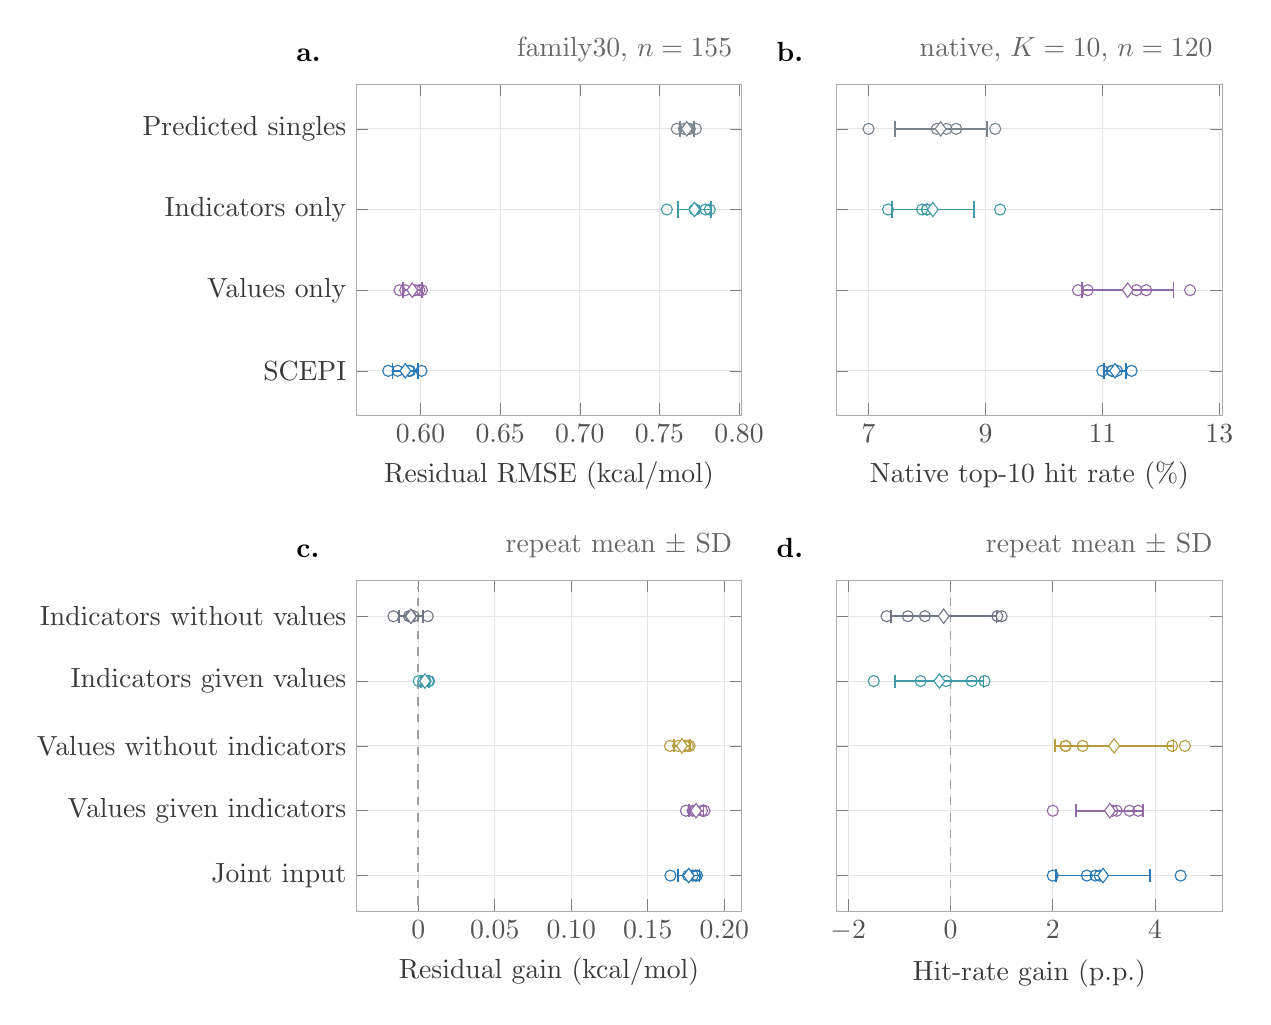
\begin{tikzpicture}[font=\sffamily\fontsize{10}{12}\selectfont]
\definecolor{FactorBlue}{HTML}{2878B5}
\definecolor{ValuesPurple}{HTML}{9368A6}
\definecolor{MaskTeal}{HTML}{3F9BA8}
\definecolor{NeutralGray}{HTML}{7B858E}
\definecolor{ContrastGold}{HTML}{B89B3C}
\definecolor{ContrastGray}{HTML}{6F7785}
\begin{axis}[
at={(47mm,58mm)}, anchor=south west,
width=49mm, height=42mm,
scale only axis,
xmin=0.559529685204, xmax=0.801796303154, ymin=-0.55, ymax=3.55,
axis line style={draw=gray!65},
grid=major, grid style={draw=gray!20, line width=0.35pt},
tick label style={font=\fontsize{10}{12}\selectfont, text=black!68},
label style={font=\fontsize{10}{12}\selectfont, text=black!78},
xticklabel style={/pgf/number format/fixed, /pgf/number format/precision=2},
xtick={0.6,0.65,0.7,0.75,0.8},
ytick={0,1,2,3},
yticklabels={SCEPI,Values only,Indicators only,Predicted singles},
yticklabel style={font=\fontsize{10}{12}\selectfont, text=black!78},
xlabel={Residual RMSE (kcal/mol)}, ylabel={},
clip=false,
xticklabels={0.60,0.65,0.70,0.75,0.80},
]
\node[anchor=south west, font=\bfseries\fontsize{10}{12}\selectfont] at (rel axis cs:-0.18,1.04) {a.};
\node[anchor=south east, font=\fontsize{10}{12}\selectfont, text=black!60] at (rel axis cs:1,1.04) {family30, $n=155$};
\draw[FactorBlue, line width=0.65pt] (axis cs:0.582415650814,0) -- (axis cs:0.598417156258,0);
\draw[FactorBlue, line width=0.65pt] (axis cs:0.582415650814,-0.1) -- (axis cs:0.582415650814,0.1);
\draw[FactorBlue, line width=0.65pt] (axis cs:0.598417156258,-0.1) -- (axis cs:0.598417156258,0.1);
\addplot[only marks, mark=o, mark size=2.0pt, color=FactorBlue, mark options={draw=FactorBlue, fill=white}] coordinates {(0.593461937428,0) (0.585588060775,0) (0.600602174461,0) (0.579718570033,0) (0.592711274986,0)};
\addplot[only marks, mark=diamond*, mark size=2.6pt, color=FactorBlue, mark options={draw=FactorBlue, fill=white}] coordinates {(0.590416403536,0)};
\draw[ValuesPurple, line width=0.65pt] (axis cs:0.58882164198,1) -- (axis cs:0.600809987882,1);
\draw[ValuesPurple, line width=0.65pt] (axis cs:0.58882164198,0.9) -- (axis cs:0.58882164198,1.1);
\draw[ValuesPurple, line width=0.65pt] (axis cs:0.600809987882,0.9) -- (axis cs:0.600809987882,1.1);
\addplot[only marks, mark=o, mark size=2.0pt, color=ValuesPurple, mark options={draw=ValuesPurple, fill=white}] coordinates {(0.596725221325,1) (0.590387929789,1) (0.600888353105,1) (0.586822795804,1) (0.599254774631,1)};
\addplot[only marks, mark=diamond*, mark size=2.6pt, color=ValuesPurple, mark options={draw=ValuesPurple, fill=white}] coordinates {(0.594815814931,1)};
\draw[MaskTeal, line width=0.65pt] (axis cs:0.761485221221,2) -- (axis cs:0.782494671619,2);
\draw[MaskTeal, line width=0.65pt] (axis cs:0.761485221221,1.9) -- (axis cs:0.761485221221,2.1);
\draw[MaskTeal, line width=0.65pt] (axis cs:0.782494671619,1.9) -- (axis cs:0.782494671619,2.1);
\addplot[only marks, mark=o, mark size=2.0pt, color=MaskTeal, mark options={draw=MaskTeal, fill=white}] coordinates {(0.778929230665,2) (0.772716186936,2) (0.781607418325,2) (0.754663139739,2) (0.772033756436,2)};
\addplot[only marks, mark=diamond*, mark size=2.6pt, color=MaskTeal, mark options={draw=MaskTeal, fill=white}] coordinates {(0.77198994642,2)};
\draw[NeutralGray, line width=0.65pt] (axis cs:0.762748653642,3) -- (axis cs:0.771640933055,3);
\draw[NeutralGray, line width=0.65pt] (axis cs:0.762748653642,2.9) -- (axis cs:0.762748653642,3.1);
\draw[NeutralGray, line width=0.65pt] (axis cs:0.771640933055,2.9) -- (axis cs:0.771640933055,3.1);
\addplot[only marks, mark=o, mark size=2.0pt, color=NeutralGray, mark options={draw=NeutralGray, fill=white}] coordinates {(0.772869861166,3) (0.767736311166,3) (0.765399088696,3) (0.760887015469,3) (0.769081690245,3)};
\addplot[only marks, mark=diamond*, mark size=2.6pt, color=NeutralGray, mark options={draw=NeutralGray, fill=white}] coordinates {(0.767194793349,3)};
\end{axis}
\begin{axis}[
at={(108mm,58mm)}, anchor=south west,
width=49mm, height=42mm,
scale only axis,
xmin=6.45, xmax=13.05, ymin=-0.55, ymax=3.55,
axis line style={draw=gray!65},
grid=major, grid style={draw=gray!20, line width=0.35pt},
tick label style={font=\fontsize{10}{12}\selectfont, text=black!68},
label style={font=\fontsize{10}{12}\selectfont, text=black!78},
xticklabel style={/pgf/number format/fixed, /pgf/number format/precision=2},
xtick={7,9,11,13},
ytick={0,1,2,3},
yticklabels={,,,},
yticklabel style={font=\fontsize{10}{12}\selectfont, text=black!78},
xlabel={Native top-10 hit rate (\%)}, ylabel={},
clip=false,
xticklabels={7,9,11,13},
]
\node[anchor=south west, font=\bfseries\fontsize{10}{12}\selectfont] at (rel axis cs:-0.18,1.04) {b.};
\node[anchor=south east, font=\fontsize{10}{12}\selectfont, text=black!60] at (rel axis cs:1,1.04) {native, $K=10$, $n=120$};
\draw[FactorBlue, line width=0.65pt] (axis cs:11.034092480832,0) -- (axis cs:11.399240852502,0);
\draw[FactorBlue, line width=0.65pt] (axis cs:11.034092480832,-0.1) -- (axis cs:11.034092480832,0.1);
\draw[FactorBlue, line width=0.65pt] (axis cs:11.399240852502,-0.1) -- (axis cs:11.399240852502,0.1);
\addplot[only marks, mark=o, mark size=2.0pt, color=FactorBlue, mark options={draw=FactorBlue, fill=white}] coordinates {(11.5,0) (11.25,0) (11,0) (11.166666666667,0) (11.166666666667,0)};
\addplot[only marks, mark=diamond*, mark size=2.6pt, color=FactorBlue, mark options={draw=FactorBlue, fill=white}] coordinates {(11.216666666667,0)};
\draw[ValuesPurple, line width=0.65pt] (axis cs:10.650709541208,1) -- (axis cs:12.215957125458,1);
\draw[ValuesPurple, line width=0.65pt] (axis cs:10.650709541208,0.9) -- (axis cs:10.650709541208,1.1);
\draw[ValuesPurple, line width=0.65pt] (axis cs:12.215957125458,0.9) -- (axis cs:12.215957125458,1.1);
\addplot[only marks, mark=o, mark size=2.0pt, color=ValuesPurple, mark options={draw=ValuesPurple, fill=white}] coordinates {(11.583333333333,1) (10.583333333333,1) (12.5,1) (10.75,1) (11.75,1)};
\addplot[only marks, mark=diamond*, mark size=2.6pt, color=ValuesPurple, mark options={draw=ValuesPurple, fill=white}] coordinates {(11.433333333333,1)};
\draw[MaskTeal, line width=0.65pt] (axis cs:7.399305899681,2) -- (axis cs:8.800694100319,2);
\draw[MaskTeal, line width=0.65pt] (axis cs:7.399305899681,1.9) -- (axis cs:7.399305899681,2.1);
\draw[MaskTeal, line width=0.65pt] (axis cs:8.800694100319,1.9) -- (axis cs:8.800694100319,2.1);
\addplot[only marks, mark=o, mark size=2.0pt, color=MaskTeal, mark options={draw=MaskTeal, fill=white}] coordinates {(8,2) (9.25,2) (7.333333333333,2) (8,2) (7.916666666667,2)};
\addplot[only marks, mark=diamond*, mark size=2.6pt, color=MaskTeal, mark options={draw=MaskTeal, fill=white}] coordinates {(8.1,2)};
\draw[NeutralGray, line width=0.65pt] (axis cs:7.446285403125,3) -- (axis cs:9.020381263541,3);
\draw[NeutralGray, line width=0.65pt] (axis cs:7.446285403125,2.9) -- (axis cs:7.446285403125,3.1);
\draw[NeutralGray, line width=0.65pt] (axis cs:9.020381263541,2.9) -- (axis cs:9.020381263541,3.1);
\addplot[only marks, mark=o, mark size=2.0pt, color=NeutralGray, mark options={draw=NeutralGray, fill=white}] coordinates {(7,3) (8.333333333333,3) (8.166666666667,3) (8.5,3) (9.166666666667,3)};
\addplot[only marks, mark=diamond*, mark size=2.6pt, color=NeutralGray, mark options={draw=NeutralGray, fill=white}] coordinates {(8.233333333333,3)};
\end{axis}
\begin{axis}[
at={(47mm,-5mm)}, anchor=south west,
width=49mm, height=42mm,
scale only axis,
xmin=-0.040608704323, xmax=0.211528500856, ymin=-0.55, ymax=4.55,
axis line style={draw=gray!65},
grid=major, grid style={draw=gray!20, line width=0.35pt},
tick label style={font=\fontsize{10}{12}\selectfont, text=black!68},
label style={font=\fontsize{10}{12}\selectfont, text=black!78},
xticklabel style={/pgf/number format/fixed, /pgf/number format/precision=2},
xtick={0,0.05,0.1,0.15,0.2},
ytick={0,1,2,3,4},
yticklabels={Joint input,Values given indicators,Values without indicators,Indicators given values,Indicators without values},
yticklabel style={font=\fontsize{10}{12}\selectfont, text=black!78},
xlabel={Residual gain (kcal/mol)}, ylabel={},
clip=false,
xticklabels={0,0.05,0.10,0.15,0.20},
]
\node[anchor=south west, font=\bfseries\fontsize{10}{12}\selectfont] at (rel axis cs:-0.18,1.04) {c.};
\node[anchor=south east, font=\fontsize{10}{12}\selectfont, text=black!60] at (rel axis cs:1,1.04) {repeat mean $\pm$ SD};
\draw[dashed, gray!75, line width=0.6pt] (axis cs:0,-0.45) -- (axis cs:0,4.45);
\draw[FactorBlue, line width=0.65pt] (axis cs:0.169729548774,0) -- (axis cs:0.18382723085,0);
\draw[FactorBlue, line width=0.65pt] (axis cs:0.169729548774,-0.1) -- (axis cs:0.169729548774,0.1);
\draw[FactorBlue, line width=0.65pt] (axis cs:0.18382723085,-0.1) -- (axis cs:0.18382723085,0.1);
\addplot[only marks, mark=o, mark size=2.0pt, color=FactorBlue, mark options={draw=FactorBlue, fill=white}] coordinates {(0.179407923738,0) (0.182148250392,0) (0.164796914235,0) (0.181168445436,0) (0.17637041526,0)};
\addplot[only marks, mark=diamond*, mark size=2.6pt, color=FactorBlue, mark options={draw=FactorBlue, fill=white}] coordinates {(0.176778389812,0)};
\draw[ValuesPurple, line width=0.65pt] (axis cs:0.176691222382,1) -- (axis cs:0.186455863386,1);
\draw[ValuesPurple, line width=0.65pt] (axis cs:0.176691222382,0.9) -- (axis cs:0.176691222382,1.1);
\draw[ValuesPurple, line width=0.65pt] (axis cs:0.186455863386,0.9) -- (axis cs:0.186455863386,1.1);
\addplot[only marks, mark=o, mark size=2.0pt, color=ValuesPurple, mark options={draw=ValuesPurple, fill=white}] coordinates {(0.185467293237,1) (0.187128126161,1) (0.181005243864,1) (0.174944569706,1) (0.179322481451,1)};
\addplot[only marks, mark=diamond*, mark size=2.6pt, color=ValuesPurple, mark options={draw=ValuesPurple, fill=white}] coordinates {(0.181573542884,1)};
\draw[ContrastGold, line width=0.65pt] (axis cs:0.16713165816,2) -- (axis cs:0.177626298675,2);
\draw[ContrastGold, line width=0.65pt] (axis cs:0.16713165816,1.9) -- (axis cs:0.16713165816,2.1);
\draw[ContrastGold, line width=0.65pt] (axis cs:0.177626298675,1.9) -- (axis cs:0.177626298675,2.1);
\addplot[only marks, mark=o, mark size=2.0pt, color=ContrastGold, mark options={draw=ContrastGold, fill=white}] coordinates {(0.176144639841,2) (0.177348381377,2) (0.164510735591,2) (0.174064219665,2) (0.169826915614,2)};
\addplot[only marks, mark=diamond*, mark size=2.6pt, color=ContrastGold, mark options={draw=ContrastGold, fill=white}] coordinates {(0.172378978418,2)};
\draw[MaskTeal, line width=0.65pt] (axis cs:0.001647913126,3) -- (axis cs:0.007150909663,3);
\draw[MaskTeal, line width=0.65pt] (axis cs:0.001647913126,2.9) -- (axis cs:0.001647913126,3.1);
\draw[MaskTeal, line width=0.65pt] (axis cs:0.007150909663,2.9) -- (axis cs:0.007150909663,3.1);
\addplot[only marks, mark=o, mark size=2.0pt, color=MaskTeal, mark options={draw=MaskTeal, fill=white}] coordinates {(0.003263283897,3) (0.004799869015,3) (0.000286178644,3) (0.007104225771,3) (0.006543499646,3)};
\addplot[only marks, mark=diamond*, mark size=2.6pt, color=MaskTeal, mark options={draw=MaskTeal, fill=white}] coordinates {(0.004399411395,3)};
\draw[ContrastGray, line width=0.65pt] (axis cs:-0.012806222441,4) -- (axis cs:0.003215916298,4);
\draw[ContrastGray, line width=0.65pt] (axis cs:-0.012806222441,3.9) -- (axis cs:-0.012806222441,4.1);
\draw[ContrastGray, line width=0.65pt] (axis cs:0.003215916298,3.9) -- (axis cs:0.003215916298,4.1);
\addplot[only marks, mark=o, mark size=2.0pt, color=ContrastGray, mark options={draw=ContrastGray, fill=white}] coordinates {(-0.006059369499,4) (-0.00497987577,4) (-0.016208329629,4) (0.00622387573,4) (-0.002952066191,4)};
\addplot[only marks, mark=diamond*, mark size=2.6pt, color=ContrastGray, mark options={draw=ContrastGray, fill=white}] coordinates {(-0.004795153072,4)};
\end{axis}
\begin{axis}[
at={(108mm,-5mm)}, anchor=south west,
width=49mm, height=42mm,
scale only axis,
xmin=-2.23, xmax=5.313333333333, ymin=-0.55, ymax=4.55,
axis line style={draw=gray!65},
grid=major, grid style={draw=gray!20, line width=0.35pt},
tick label style={font=\fontsize{10}{12}\selectfont, text=black!68},
label style={font=\fontsize{10}{12}\selectfont, text=black!78},
xticklabel style={/pgf/number format/fixed, /pgf/number format/precision=2},
xtick={-2,0,2,4},
ytick={0,1,2,3,4},
yticklabels={,,,,},
yticklabel style={font=\fontsize{10}{12}\selectfont, text=black!78},
xlabel={Hit-rate gain (p.p.)}, ylabel={},
clip=false,
xticklabels={$-2$,0,2,4},
]
\node[anchor=south west, font=\bfseries\fontsize{10}{12}\selectfont] at (rel axis cs:-0.18,1.04) {d.};
\node[anchor=south east, font=\fontsize{10}{12}\selectfont, text=black!60] at (rel axis cs:1,1.04) {repeat mean $\pm$ SD};
\draw[dashed, gray!75, line width=0.6pt] (axis cs:0,-0.45) -- (axis cs:0,4.45);
\draw[FactorBlue, line width=0.65pt] (axis cs:2.062132426304,0) -- (axis cs:3.904534240362,0);
\draw[FactorBlue, line width=0.65pt] (axis cs:2.062132426304,-0.1) -- (axis cs:2.062132426304,0.1);
\draw[FactorBlue, line width=0.65pt] (axis cs:3.904534240362,-0.1) -- (axis cs:3.904534240362,0.1);
\addplot[only marks, mark=o, mark size=2.0pt, color=FactorBlue, mark options={draw=FactorBlue, fill=white}] coordinates {(4.5,0) (2.916666666667,0) (2.833333333333,0) (2.666666666667,0) (2,0)};
\addplot[only marks, mark=diamond*, mark size=2.6pt, color=FactorBlue, mark options={draw=FactorBlue, fill=white}] coordinates {(2.983333333333,0)};
\draw[ValuesPurple, line width=0.65pt] (axis cs:2.461558533099,1) -- (axis cs:3.771774800234,1);
\draw[ValuesPurple, line width=0.65pt] (axis cs:2.461558533099,0.9) -- (axis cs:2.461558533099,1.1);
\draw[ValuesPurple, line width=0.65pt] (axis cs:3.771774800234,0.9) -- (axis cs:3.771774800234,1.1);
\addplot[only marks, mark=o, mark size=2.0pt, color=ValuesPurple, mark options={draw=ValuesPurple, fill=white}] coordinates {(3.5,1) (2,1) (3.666666666667,1) (3.166666666667,1) (3.25,1)};
\addplot[only marks, mark=diamond*, mark size=2.6pt, color=ValuesPurple, mark options={draw=ValuesPurple, fill=white}] coordinates {(3.116666666667,1)};
\draw[ContrastGold, line width=0.65pt] (axis cs:2.039899429647,2) -- (axis cs:4.360100570353,2);
\draw[ContrastGold, line width=0.65pt] (axis cs:2.039899429647,1.9) -- (axis cs:2.039899429647,2.1);
\draw[ContrastGold, line width=0.65pt] (axis cs:4.360100570353,1.9) -- (axis cs:4.360100570353,2.1);
\addplot[only marks, mark=o, mark size=2.0pt, color=ContrastGold, mark options={draw=ContrastGold, fill=white}] coordinates {(4.583333333333,2) (2.25,2) (4.333333333333,2) (2.25,2) (2.583333333333,2)};
\addplot[only marks, mark=diamond*, mark size=2.6pt, color=ContrastGold, mark options={draw=ContrastGold, fill=white}] coordinates {(3.2,2)};
\draw[MaskTeal, line width=0.65pt] (axis cs:-1.079880944172,3) -- (axis cs:0.646547610839,3);
\draw[MaskTeal, line width=0.65pt] (axis cs:-1.079880944172,2.9) -- (axis cs:-1.079880944172,3.1);
\draw[MaskTeal, line width=0.65pt] (axis cs:0.646547610839,2.9) -- (axis cs:0.646547610839,3.1);
\addplot[only marks, mark=o, mark size=2.0pt, color=MaskTeal, mark options={draw=MaskTeal, fill=white}] coordinates {(-0.083333333333,3) (0.666666666667,3) (-1.5,3) (0.416666666667,3) (-0.583333333333,3)};
\addplot[only marks, mark=diamond*, mark size=2.6pt, color=MaskTeal, mark options={draw=MaskTeal, fill=white}] coordinates {(-0.216666666667,3)};
\draw[ContrastGray, line width=0.65pt] (axis cs:-1.165119809952,4) -- (axis cs:0.898453143285,4);
\draw[ContrastGray, line width=0.65pt] (axis cs:-1.165119809952,3.9) -- (axis cs:-1.165119809952,4.1);
\draw[ContrastGray, line width=0.65pt] (axis cs:0.898453143285,3.9) -- (axis cs:0.898453143285,4.1);
\addplot[only marks, mark=o, mark size=2.0pt, color=ContrastGray, mark options={draw=ContrastGray, fill=white}] coordinates {(1,4) (0.916666666667,4) (-0.833333333333,4) (-0.5,4) (-1.25,4)};
\addplot[only marks, mark=diamond*, mark size=2.6pt, color=ContrastGray, mark options={draw=ContrastGray, fill=white}] coordinates {(-0.133333333333,4)};
\end{axis}
\end{tikzpicture}
\caption{Measured numerical effects supply the main conditioning gain under 30\% homology grouping. (a) Residual RMSE and (b) native top-10 hit rate for the four input conditions. Values only uses measured numerical inputs with zero indicators; indicators only uses predicted values with observed indicators. Predicted singles removes both measured inputs. External calibration and fitting conditions are matched. (c) Residual reduction and (d) hit-rate gain for the joint and separate input contrasts. Positive gains favor adding the named input. Open points are equal-protein repetition means; diamonds and whiskers show their mean and standard deviation. Residual and selection cohorts contain 155 and 120 held-out proteins.}
\label{fig:components}
\end{figure}

When every method uses the same measured single-effect sum, SCEPI retains an 11.27\% compensation hit rate (Appendix Table~\ref{tab:commonmain}). Additivity gives 4.42\% and global nonlinearity 4.70\%; ThermoMPNN-D reaches 5.30\%, Kermut 5.47\%, and StabilityArc + Kermut 8.17\%. Mean MLP and mean ridge reach 7.17\% and 7.33\%. Recovery gains over the first four controls are 0.170, 0.155, 0.218, and 0.194 kcal/mol, respectively, with a 0.090 kcal/mol gain over StabilityArc + Kermut. Only the predicted four-term nonadditivity differs between paired scores.

Restricting evaluation to measurements at least 0.5 kcal/mol from both assay limits preserves this advantage (Appendix Table~\ref{tab:commonmain}). Hit rates are 11.15\% for SCEPI, 4.52\% for additivity, 4.82\% for global nonlinearity, 5.27\% for ThermoMPNN-D, and 5.29\% for Kermut. StabilityArc + Kermut reaches 8.12\%, mean MLP 7.30\%, and mean ridge 7.48\%.

\subsection{Reference constraints improve residual prediction}

Cycle subtraction enforces the reference constraints and improves residual accuracy against the same-capacity direct head (Tables~\ref{tab:allcomponents} and~\ref{tab:threshold25}). The direct head reaches residual RMSE 0.632 kcal/mol under the primary grouping and 0.630 kcal/mol under the stricter grouping, compared with SCEPI's 0.590 and 0.604 kcal/mol. Native hit-rate gains are 0.68 and $-0.23$ percentage points, respectively. The residual benefit holds across both groupings; the hit-rate effect varies.

Setting the pair term to zero at inference lowers native hit rate from 11.22\% to 4.42\% and raises residual RMSE from 0.590 to 1.076 kcal/mol (Table~\ref{tab:allcomponents}). The trained single head and phenotype map remain fixed during this intervention. Complete representation, mapping, and training-objective comparisons are reported in the appendix.

\interlinepenalty=0
\section{Discussion}

Single-mutant measurements can guide compensatory discovery before any target combination labels are collected. SCEPI uses them to condition an interaction function learned across source proteins. The retrospective comparisons quantify the resulting selection benefit at a fixed budget and across held-out homology groups. This use of target information extends beyond fitting individual effects or a Gaussian-process posterior. StabilityArc supplies a source-trained prior for target adaptation \citep{feller2026}; SCEPI also supplies observed single effects to the shared interaction function. Independently refitted input controls retain the external calibration rule and distinguish numerical effects from availability indicators. Selection gains also persist with the same measured single-effect sum.

The reference constraints fix the model's behavior at wild-type endpoints and improve mean residual accuracy against a direct head. Their hit-rate effects vary across groupings. Measured-input conditioning improves both residual prediction and compensatory selection under the two homology groupings.

\section{Conclusion}

By conditioning a transferable interaction function on measured single effects, SCEPI improves residual prediction and compensatory discovery in matched controls and held-out comparisons. Code, configurations, and reproduction materials are available at \url{https://github.com/SZU-ADDG/SCEPI}, version \texttt{recomb2027-20261021}.

\clearpage
\begin{thebibliography}{10}

\bibitem{azbukina2022}
N. Azbukina, A. Zharikova, and V. Ramensky.
\newblock Intragenic compensation through the lens of deep mutational scanning.
\newblock \emph{Biophysical Reviews}, 14(5):1161--1182, 2022.
\newblock doi:10.1007/s12551-022-01005-w.

\bibitem{davis2009}
B. H. Davis, A. F. Y. Poon, and M. C. Whitlock.
\newblock Compensatory mutations are repeatable and clustered within proteins.
\newblock \emph{Proceedings of the Royal Society B}, 276(1663):1823--1827, 2009.
\newblock doi:10.1098/rspb.2008.1846.

\bibitem{dieckhaus2025}
H. Dieckhaus and B. Kuhlman.
\newblock Protein stability models fail to capture epistatic interactions of double point mutations.
\newblock \emph{Protein Science}, 34(1):e70003, 2025.
\newblock doi:10.1002/pro.70003.

\bibitem{faure2024}
A. J. Faure and B. Lehner.
\newblock MoCHI: neural networks to fit interpretable models and quantify energies, energetic couplings, epistasis, and allostery from deep mutational scanning data.
\newblock \emph{Genome Biology}, 25:303, 2024.
\newblock doi:10.1186/s13059-024-03444-y.

\bibitem{gong2013}
L. I. Gong, M. A. Suchard, and J. D. Bloom.
\newblock Stability-mediated epistasis constrains the evolution of an influenza protein.
\newblock \emph{eLife}, 2:e00631, 2013.
\newblock doi:10.7554/eLife.00631.

\bibitem{groth2024}
P. M. Groth, M. H. Kerrn, L. Olsen, J. Salomon, and W. Boomsma.
\newblock Kermut: Composite kernel regression for protein variant effects.
\newblock In \emph{Advances in Neural Information Processing Systems}, volume 37, 2024.
\newblock doi:10.52202/079017-0929.

\bibitem{horovitz1996}
A. Horovitz.
\newblock Double-mutant cycles: a powerful tool for analyzing protein structure and function.
\newblock \emph{Folding \& Design}, 1(6):R121--R126, 1996.
\newblock doi:10.1016/S1359-0278(96)00056-9.

\bibitem{lin2023}
Z. Lin et al.
\newblock Evolutionary-scale prediction of atomic-level protein structure with a language model.
\newblock \emph{Science}, 379(6637):1123--1130, 2023.
\newblock doi:10.1126/science.ade2574.

\bibitem{ouyang2023}
J. Ouyang-Zhang, D. Diaz, A. Klivans, and P. Krahenbuehl.
\newblock Predicting a protein's stability under a million mutations.
\newblock In \emph{Advances in Neural Information Processing Systems}, volume 36, 2023.
\newblock doi:10.52202/075280-3332.

\bibitem{otwinowski2018}
J. Otwinowski, D. M. McCandlish, and J. B. Plotkin.
\newblock Inferring the shape of global epistasis.
\newblock \emph{Proceedings of the National Academy of Sciences}, 115(32):E7550--E7558, 2018.
\newblock doi:10.1073/pnas.1804015115.

\bibitem{tareen2022}
A. Tareen, M. Kooshkbaghi, A. Posfai, et al.
\newblock MAVE-NN: learning genotype-phenotype maps from multiplex assays of variant effect.
\newblock \emph{Genome Biology}, 23:98, 2022.
\newblock doi:10.1186/s13059-022-02661-7.

\bibitem{reeves2026}
S. Reeves and S. Kalyaanamoorthy.
\newblock Robust multi-mutant protein stability prediction from a fine-tuned evolutionary scale model.
\newblock bioRxiv preprint, 2026.
\newblock doi:10.64898/2026.06.04.730231.

\bibitem{tsuboyama2023}
K. Tsuboyama et al.
\newblock Mega-scale experimental analysis of protein folding stability in biology and design.
\newblock \emph{Nature}, 620:434--444, 2023.
\newblock doi:10.1038/s41586-023-06328-6.

\bibitem{feller2026}
A. L. Feller, A. D. Ellington, and C. O. Wilke.
\newblock StabilityArc: Decoding protein sequence embeddings into generalizable stability landscapes.
\newblock arXiv preprint arXiv:2610.00742, 2026.

\bibitem{park2024}
Y. Park, B. P. H. Metzger, and J. W. Thornton.
\newblock The simplicity of protein sequence-function relationships.
\newblock \emph{Nature Communications}, 15:7953, 2024.
\newblock doi:10.1038/s41467-024-51895-5.

\bibitem{notin2023}
P. Notin et al.
\newblock ProteinGym: Large-Scale Benchmarks for Protein Fitness Prediction and Design.
\newblock In \emph{Advances in Neural Information Processing Systems}, volume 36, pages 64331--64379, 2023.

\bibitem{didi2026}
K. Didi et al.
\newblock FLIP2: Expanding Protein Fitness Landscape Benchmarks for Real-World Machine Learning Applications.
\newblock In \emph{Proceedings of the 43rd International Conference on Machine Learning}, 2026.

\end{thebibliography}
\clearpage
\pagenumbering{arabic}
\renewcommand{\thepage}{S\arabic{page}}
\appendix
\section*{Supplementary material}
\section{Model parameterization and algebraic properties}
\label{app:parameterization}

Residue representations from the frozen ESM-2 model have dimension 1,280. Independent linear projections map wild-type, local-change, and cross-site-change features to the selected projection dimension. Amino-acid states use one-hot encodings. Both heads contain hidden layers of dimensions 256 and 128, GELU activations, and a scalar output. The pair head additionally receives calibrated single effects and observation indicators. Its sequence relation contains the logarithm of one plus the site gap and the gap divided by sequence length. Source-validation measurements select projection dimensions, learning rates, auxiliary weights, and $\omega$.

The cross-site context is the change at one site after the other site is substituted,
\begin{equation}
\chi_{i\leftarrow j}(b)=h_i(x_p(j,b))-h_i(s_p).
\end{equation}
Encoding each single-mutant sequence once supplies residue states for every candidate pair involving that mutation. This gives the pair network mutation-dependent context without encoding double-mutant sequences. Sequence separation describes the endpoint relation; the structural variant adds reference C$\alpha$ distances and residue confidence.

The normalized phenotype map is
\begin{equation}
g(z)=\frac{z+\sum_{k=1}^{20}b_k[\tanh(c_kz+d_k)-\tanh(d_k)]}
{1+\sum_{k=1}^{20}b_kc_k\operatorname{sech}^2(d_k)},\qquad b_k,c_k>0.
\end{equation}
Softplus ensures positive parameters. Substitution of $z=0$ gives $g(0)=0$, and differentiation gives $g'(0)=1$. The derivative is positive for every $z$, with the linear term preserving nonzero slopes in the tails. A positive factor $\tau$ sets the phenotype scale.

For $u=\widetilde a_i(a)$ and $v=\widetilde a_j(b)$, the predicted phenotype contrast decomposes as
\begin{align}
\widehat\epsilon_{\mathrm{global}}&=\tau[g(u+v)-g(u)-g(v)],\\
\widehat\epsilon_{\mathrm{pair}}&=\tau[g(u+v+r_{ij})-g(u+v)].
\end{align}
Their sum is $\widehat\epsilon_p$. With the identity map and unit scale, the phenotype contrast equals $r_{ij}$. With a nonlinear map, the complete contrast includes both contributions.

Symmetry of $F$ carries over to the cycle subtraction. At $b=w_j$, the first two terms cancel and so do the last two, giving $r_{ij}(a,w_j)=0$. The other reference constraint follows identically. An endpoint term $v_i(a)$ contributes $v_i(a)-v_i(a)-v_i(w_i)+v_i(w_i)=0$ to the subtraction. The second endpoint term and the constant cancel in the same way. Endpoint exchange and reference-state outputs are also checked on real data.

\subsection*{Matched controls for the pair function}

For each endpoint state, let $q_i(a)=\mathbf{1}[a\neq w_i]$. The pair network receives $q_i(a)\widetilde a_i(a)$ and $q_i(a)m_i(a)$. Reference-state values and indicators are therefore zero. In S-all, the effective indicators in the four cycle evaluations are $(1,1)$, $(1,0)$, $(0,1)$, and $(0,0)$ whenever both constituent measurements are available. Local changes and substitution scores vanish at a reference endpoint. Cross-site changes vanish when the other endpoint is restored.

The input controls vary calibrated versus model-predicted effects and observed versus zero indicators independently. The values-only control keeps $\widetilde a_i(a),\widetilde a_j(b)$ and removes the indicators. The indicators-only control supplies $a_i(a),a_j(b)$ with the original indicators. Joint input removal supplies predicted effects and zero indicators. Every control retains the state-specific gating, input dimensions, and parameter count. External calibration follows Equation~\eqref{eq:calibration} and the same label-permission rule in all four cases.

The direct-head control predicts $r_{ij}(a,b)=F(i,a;j,b)$ with the same symmetric network. Its projections, endpoint features, measured inputs, hidden dimensions, and parameter count match SCEPI. Cycle subtraction evaluates the symmetric function four times per candidate; the direct head evaluates it once. Both reuse the same frozen sequence representations. The comparison measures the predictive effect and additional pair-function computation of cycle subtraction. A matched configuration with 64-dimensional projections has 836,927 parameters in each predictor. Cached-feature inference on 32 real held-out cycles takes median 6.88 ms for cycle subtraction and 3.39 ms for the direct head using four CPU threads. These medians use 100 timed batches after 20 warm-up batches per predictor. They exclude frozen-encoder computation and feature-cache construction.

All matched controls reuse the full model's source-selected objective and hyperparameters in each outer partition. Each repetition matches the pretrained single checkpoint, random initialization, source rows, sampler, optimizer, and checkpoint-selection rule. Maximum epochs and early-stopping patience are identical, while realized stopping epochs and fitted weights may differ. The label-mixing weight follows the same source-validation procedure.

Evaluation holds proteins, candidate pools, measurement margins, budgets, and aggregation fixed. Repeating the comparisons independently under the stricter homology grouping tests the predictive contributions of cycle subtraction and measured pair inputs across both groupings.

\section{Repetitions, aggregation, and statistical analysis}

Five outer partitions define the 30\% grouping. A source-trained model uses one partition for testing, the next for validation, and the remaining three for training. Training seeds 11, 23, 47, 89, and 131 give all 25 outer-fold and training-seed evaluations per model. Every eligible target protein is evaluated once per seed in its assigned test partition, using all eligible target double mutants. The resulting paired protein-repetition records number 795 for phenotype prediction, 775 for residual prediction, and 600 for standard compensation selection. The 0.5 kcal/mol margin cohort contains 575 records. Each protein's five repetitions are averaged before computing the equal-protein mean.

At each repetition, all compared methods use the same permitted target labels and candidate definition. Means use the paired cohort. Phenotype and residual comparisons cover 159 and 155 proteins, respectively, from 51 homology groups. Standard compensation covers 120 proteins and 44 groups. The 0.5 kcal/mol margin comparison covers 115 proteins and 43 groups. Source-validation configurations are retained across training repetitions. Candidate yield is excluded from source hyperparameter selection. Five outer partitions describe source-data separation; five training seeds describe repeated model fitting.

Uncertainty uses 10,000 homology-group bootstrap draws with statistical seed 20261013. Each draw samples groups with replacement and retains all member proteins. Its effect is the equal-protein mean over the sampled groups. Repeated model fits are averaged within protein before resampling. Comparisons with the same group membership use the same resampling draws. A bootstrap positive fraction is the fraction of resampled mean differences above zero. It describes uncertainty in the observed paired mean under this resampling scheme. Tables~\ref{tab:nativeuncertainty} and~\ref{tab:marginuncertainty} report the top-10 endpoint. Table~\ref{tab:pairfunctionuncertainty} reports the matched pair-function controls.

\begin{table}[H]
\centering
\caption{Paired native top-10 hit-rate advantage of SCEPI. Gains and 95\% bootstrap intervals are in percentage points. Positive fractions refer to resampled mean gains. Every comparison includes 120 proteins, 44 groups, and five model repetitions.}
\label{tab:nativeuncertainty}
\begin{tabular}{lrrr}
\toprule
Comparator & Mean gain & 95\% interval & Positive fraction \\
\midrule
Additive & 4.83 & [1.97, 7.87] & 0.9988 \\
Global nonlinear & 6.77 & [3.20, 9.98] & 1.0000 \\
ThermoMPNN-D & 4.15 & [$-0.41$, 7.02] & 0.9620 \\
Kermut & 5.82 & [2.52, 8.85] & 0.9996 \\
StabilityArc + Kermut & 2.47 & [$-1.38$, 5.47] & 0.9166 \\
Mean MLP & 1.15 & [$-2.89$, 3.84] & 0.7374 \\
Mean ridge & $-0.20$ & [$-4.21$, 1.97] & 0.4297 \\
\bottomrule
\end{tabular}
\end{table}

\begin{table}[H]
\centering
\caption{Paired top-10 hit-rate advantage with the same measured single-effect sum at margin $\geq0.5$ kcal/mol. Gains and 95\% bootstrap intervals are in percentage points. Every comparison includes 115 proteins, 43 groups, and five model repetitions.}
\label{tab:marginuncertainty}
\begin{tabular}{lrr}
\toprule
Comparator & Mean gain & 95\% interval \\
\midrule
Additive & 6.63 & [2.73, 9.80] \\
Global nonlinear & 6.33 & [2.23, 9.27] \\
ThermoMPNN-D & 5.88 & [2.41, 8.49] \\
Kermut & 5.86 & [1.97, 9.22] \\
StabilityArc + Kermut & 3.03 & [$-0.80$, 6.37] \\
Mean MLP & 3.84 & [0.18, 5.77] \\
Mean ridge & 3.67 & [0.72, 6.10] \\
\bottomrule
\end{tabular}
\end{table}

\begin{table}[H]
\centering
\setlength{\tabcolsep}{6pt}
\caption{Paired advantage of SCEPI over matched pair-function controls under the 30\% and 25\% identity groupings. Residual RMSE reductions are in kcal/mol; native top-10 hit-rate gains are in percentage points. Brackets give 95\% homology-group bootstrap intervals. Residual and selection comparisons contain 155 and 120 proteins, respectively. Each protein has five matched repetitions.}
\label{tab:pairfunctionuncertainty}
\begin{tabular}{llrr}
\toprule
Grouping & Pair-function control & Residual reduction & Hit-rate gain \\
\midrule
30\% & Predicted singles & 0.177 [0.154, 0.221] & 2.98 [0.59, 4.28] \\
30\% & Values only & 0.004 [$-0.00008$, 0.01162] & $-0.22$ [$-0.73$, 0.07] \\
30\% & Indicators only & 0.182 [0.157, 0.230] & 3.12 [0.59, 4.49] \\
30\% & Direct residual head & 0.042 [$-0.014$, 0.073] & 0.68 [$-2.86$, 2.55] \\
25\% & Predicted singles & 0.210 [0.156, 0.264] & 3.00 [0.00, 4.39] \\
25\% & Values only & 0.016 [0.001, 0.023] & 0.03 [$-0.63$, 0.40] \\
25\% & Indicators only & 0.213 [0.156, 0.273] & 3.20 [$-0.37$, 4.79] \\
25\% & Direct residual head & 0.026 [$-0.018$, 0.042] & $-0.23$ [$-1.52$, 0.79] \\
\bottomrule
\end{tabular}
\end{table}

Measured pair inputs improve both mean residual error and native hit rate in all five repetitions under each grouping. Their residual comparison has 144 protein-level wins under the primary grouping and 142 under the stricter grouping, out of 155 proteins. The reference contrast lowers mean residual error in all five repetitions at each threshold, with 108 and 97 protein-level wins. Its native hit-rate gain is positive in five repetitions under the 30\% grouping and two under the 25\% grouping.

The numerical-input and indicator contrasts use the same paired proteins. With zero indicators, measured values reduce residual RMSE by 0.172 kcal/mol under 30\% grouping and 0.193 under 25\% grouping. Their 95\% group-bootstrap intervals are [0.150, 0.215] and [0.146, 0.261]. Native hit-rate gains are 3.20 and 2.97 percentage points, with intervals [0.78, 4.61] and [0.16, 4.28]. Both metrics improve in every repetition. With predicted values, indicators change residual accuracy by $-0.005$ and $-0.003$ kcal/mol and native hit rate by $-0.13$ and $-0.20$ points. The corresponding residual intervals are [$-0.014$, 0.001] and [$-0.013$, 0.004]; hit-rate intervals are [$-0.64$, 0.33] and [$-0.48$, 0.50]. These contrasts use 10,000 common group-resampling draws with seed 20261021. Complete contrasts include native ranking, the same measured single-effect sum, recovery, and the 0.5 kcal/mol margin.

\begin{table}[H]
\centering
\caption{Paired native top-10 recovery advantage of SCEPI under 30\% grouping. Gains and 95\% group-bootstrap intervals use kcal/mol. Each comparison contains 120 proteins, 44 groups, and five fitted repetitions.}
\label{tab:recoveryuncertainty}
\begin{tabular}{lrrr}
\toprule
Comparator & Mean gain & 95\% interval & Protein wins \\
\midrule
Additive & 0.125 & [0.050, 0.168] & 84 \\
Global nonlinear & 0.175 & [0.088, 0.218] & 83 \\
ThermoMPNN-D & 0.178 & [0.046, 0.254] & 86 \\
Kermut & 0.195 & [0.119, 0.240] & 94 \\
StabilityArc + Kermut & 0.082 & [$-0.011$, 0.131] & 71 \\
Mean MLP & 0.151 & [0.013, 0.226] & 80 \\
Mean ridge & 0.092 & [$-0.035$, 0.158] & 77 \\
\bottomrule
\end{tabular}
\end{table}

Homology groups differ in size. Under 30\% grouping, residual groups contain a median of one protein and a maximum of 61; compensation groups have a median of one and a maximum of 47. Under 25\% grouping, the maxima are 75 and 56. The primary estimand gives each protein equal weight. Equal-group aggregation instead weights the within-group protein means equally. Removing the largest group and removing each group in turn provide complementary sensitivity analyses.

Against the predicted-singles control, equal-group residual gains are 0.180 and 0.172 kcal/mol under the two groupings. Removing the largest group gives 0.194 and 0.208. Every leave-one-group-out mean remains positive, ranging from 0.171 to 0.194 and from 0.195 to 0.214. Native hit-rate gains after removing the largest group are 2.00 and 1.31 percentage points. Across all group deletions, they range from 2.00 to 3.14 and from 1.31 to 3.22. Under 30\% grouping, equal-group recovery gains over ThermoMPNN-D, Kermut, StabilityArc + Kermut, and mean ridge are 0.093, 0.131, 0.031, and 0.017 kcal/mol. Removing the largest group gives 0.090, 0.176, 0.041, and 0.025. Every single-group deletion retains a positive recovery gain in these four comparisons. Full group sizes and all 220 sensitivity comparisons accompany the reproduction materials.

\section{Source model selection and implementation}
\label{app:training}

\noindent\textbf{Data preparation and partitions.} We use the joint stability estimate \texttt{dG\_ML} from processed Dataset2 and Dataset3 of Tsuboyama et al. \citep{tsuboyama2023}. Their reference backgrounds belong to groups G0 and G1 in the supplied reference list. Declared substitutions and mutant sequences are checked against each reference. Rows marked ``-'' by the data authors are excluded. The symbols ``$<-1$'' and ``$>5$'' become the intervals $(-\infty,-1]$ and $[5,\infty)$; they are retained for interval likelihoods. Numerical observations are not clipped into point targets. Repeated observations of the same biological variant are averaged, with any censored observation propagating an interval. Main evaluation requires four point-valued measurements strictly between $-1$ and 5 kcal/mol. The release preserves source rows, reference identities, measurement status, and interval endpoints.

Sequence groups are connected components of qualifying MMseqs2 alignments. Version 18.8cc5c uses exhaustive pairwise search, alignment mode 3, and the reported identity and query/target coverage fields. An edge requires identity of at least 30\% or 25\% and coverage of at least 80\% in each direction. Additional edges join shared reference scaffolds, Pfam families, and Pfam clans. Pfam 37.0 annotations use HMMER 3.4 with gathering thresholds. Connected components of the merged graph define the final partition units. The 479 reference backgrounds form 74 groups at 30\% and 67 at 25\%; the evaluated phenotype cohorts occupy 51 and 45 of those groups. All recorded edges stay within one outer partition. The released assignments, edge tables, and annotation versions specify these units directly.

The target-combination split assigns an entire site pair to training, validation, or testing. Frozen assignments show no overlap between any two sets in all 355 protein-repetition unseen-pair splits. Test sites may occur in other pairs. Proteins with only two eligible pairs use one training pair and one test pair, with no target validation labels; their hyperparameters come from source validation. These target-combination experiments are separate from S-all, which withholds every target double-mutant label.

Complete source cycles provide the residual target in Equation~\eqref{eq:observed}. For source proteins $P$, the residual objective gives equal weight to proteins and site pairs,
\begin{equation}
\mathcal L_\epsilon=
\frac{1}{|P|}\sum_{p\in P}\frac{1}{|J_p|}\sum_{(i,j)\in J_p}
\frac{1}{|Q_{pij}|}\sum_{q\in Q_{pij}}
\operatorname{Huber}\!\left(\frac{\widehat\epsilon_q-\epsilon_q}{s}\right),
\end{equation}
where $J_p$ contains measured site pairs and $Q_{pij}$ contains their cycles. The stability scale is $s=1$ kcal/mol. Sampling across proteins, then pairs, then cycles implements this weighting.

The joint objective is $\mathcal L_\epsilon+\lambda_y\mathcal L_y$. The observation term $\mathcal L_y$ is the negative log-likelihood for the predicted phenotype. Point observations use a Gaussian density; interval observations use the corresponding Gaussian interval probability. Each original observation appears once in this term. Phenotype-only fitting minimizes $\mathcal L_y$. Both objectives update the single head, pair function, and phenotype map. The objective is selected with the remaining hyperparameters within each source partition. Residual-only fitting is retained as a separate training comparison.

The single-effect model is initialized from source single-mutant fitting. Both objectives compare projection dimensions of 64 and 128 and learning rates of $10^{-4}$, $3\times10^{-4}$, and $10^{-3}$. Joint fitting additionally compares phenotype weights of 0.1 and 1. AdamW uses weight decay $10^{-4}$ and batches of 1,024 records. Training runs for at most 100 epochs, with early stopping after ten epochs without validation improvement. The residual loss uses Huber threshold 1 on the kcal/mol scale.

Single-label availability varies during training. Labels are hidden with probability 0.5; the model receives 128 labels with probability 0.25 and all single labels with probability 0.25. Source validation selects $\omega\in\{0,0.5,1\}$ in the 128-label condition. Model selection uses weighted residual RMSE, assigning weights 0.5 to zero labels, 0.25 to 128 labels, and 0.25 to all single labels. This criterion selects the objective and configuration independently within each outer partition. Nine partitions select joint fitting; fold 3 of the 30\% grouping selects phenotype-only fitting. The selected recipe is retained across its five training repetitions and matched pair-function controls. This selection uses source-validation residuals across information conditions; target candidate yield is excluded. Separately fitted loss and representation variants retain their own source-validation choices. For the additive model, validation uses phenotype error because its four-term residual is zero by construction.

Frozen sequence representations are cached by reference and single-mutant sequence. The pair predictor reuses those caches across double mutants. The structural variant adds C$\alpha$ distance and residue confidence from the reference structure. Geometry permutations preserve the recorded distance values while changing their pair assignments. Inference interventions use the fitted structural model. Retrained interventions also use the changed assignments during fitting. Each comparison retains the same outer partition and information condition.

ThermoMPNN-D is retrained on source proteins with its double-mutant head and the published single-mutant data augmentation \citep{dieckhaus2025}. Its additive counterpart is trained separately. Source fitting uses AdamW, batches of 256, at most 100 epochs, and ten-epoch validation patience. A ReduceLROnPlateau scheduler halves the learning rate. The selected source models use learning rate $10^{-4}$ and weight decay $10^{-4}$, $10^{-3}$, or $10^{-2}$. Checkpoints minimize source-validation macro residual RMSE for the double-mutant head. All 50 source fits finish within 14--45 epochs. Target adaptation uses permitted single-mutant labels.

Standalone Kermut uses its full composite kernel and Gaussian likelihood \citep{groth2024}. It fits permitted target point labels after within-target normalization. Each fit uses 150 AdamW steps, learning rate 0.1, weight decay 0.01, and one initialization. The final fitted state supplies predictions. Across 795 primary-cohort fits, the change between mean negative log marginal likelihoods in steps 130--139 and 140--149 has median 0.00233 and 90th percentile 0.00908 after division by the larger of one and the absolute latter mean. The complete optimization traces are retained in the release.

Mean ridge and mean MLP use mean-pooled residue representations with source supervision and permitted target-single adaptation. ESM-2 additive and context scores provide fixed pretrained representation controls. Table~\ref{tab:permissions} records supervision and structural inputs. The main external comparison evaluates each method's native predictions; matched SCEPI controls test the contribution of conditional inputs. Equation~\eqref{eq:selection} replaces each method's single-effect sum with the same measured sum.

\begin{table}[H]
\centering
\caption{Supervision and structural inputs in the S-all comparison. Source columns refer to phenotype labels used for supervised fitting. Every method receives zero target double-mutant labels. Structure includes the reference geometry used by the predictor or target kernel.}
\label{tab:permissions}
\begin{tabular}{lcccc}
\toprule
Method & \shortstack{Source\\singles} & \shortstack{Source\\doubles} & \shortstack{Target\\singles} & Structure \\
\midrule
SCEPI & Yes & Yes & Yes & No \\
ThermoMPNN-D & Yes & Yes & Yes & Yes \\
StabilityArc + Kermut & Yes & Yes & Yes & Yes \\
Kermut & No & No & Yes & Yes \\
Mean ridge & Yes & Yes & Yes & No \\
Mean MLP & Yes & Yes & Yes & No \\
Global nonlinear & Yes & Yes & Yes & No \\
Additive & Yes & Yes & Yes & No \\
\bottomrule
\end{tabular}
\end{table}

\section{StabilityArc architecture and target calibration}
\label{app:stabilityarc}

The StabilityArc comparison uses frozen ESMC-600M wild-type residue embeddings and attention-derived contacts \citep{feller2026}. Contact scores use symmetrization, average product correction (APC), and attention entropy weighting. Its decoder has four layers, hidden dimension 256, and eight attention heads with rotary position encoding. The full amino-acid embedding, sequence-distance features, and symmetric contact-aware pair residual are retained. Each of the ten source partitions is trained with the five fixed training seeds, giving 50 source models. Every source model excludes its target homology groups from both fitting and validation.

Each source model is trained for 40 epochs with AdamW, learning rate $10^{-4}$, and weight decay $10^{-3}$. Each assay contributes at most 40,000 measured variants per epoch. The objective combines Huber loss with 1,024 measured ranking pairs per assay. The Huber threshold is 1, and the two losses have equal weights. Double-mutant regression targets use the source-assay single-mutant median and median absolute deviation. Ranking uses measured stability order. Checkpoints are selected by source-validation double-mutant Spearman correlation. The public release supplies the architecture and a pooled checkpoint; the matched source-partition models are retrained here. Equal loss weights are an explicit implementation choice because the release does not specify them.

Target calibration uses the full Kermut covariance and Gaussian likelihood \citep{groth2024}. The retrained StabilityArc score replaces the prior mean input. All remaining kernel inputs and permitted target labels match the Kermut comparison. Target fitting uses 150 AdamW steps with learning rate 0.1 and weight decay 0.01. Only the permitted reference and single-mutant point labels are supplied. The posterior scores every eligible target double mutant and its constituent singles. The model's four-prediction contrast defines its residual.

\section{Component comparison details}

\begin{table}[H]
\centering
\caption{Top-10 compensation hit rates with the same measured single-effect sum. Each method contributes its own predicted four-term residual. The standard and margin cohorts contain 120 and 115 proteins, respectively.}
\label{tab:commonmain}
\begin{tabular}{lrr}
\toprule
Residual source & Standard pool (\%) & Margin $\geq0.5$ (\%) \\
\midrule
SCEPI & \textbf{11.27} & \textbf{11.15} \\
ThermoMPNN-D & 5.30 & 5.27 \\
Kermut & 5.47 & 5.29 \\
StabilityArc + Kermut & 8.17 & 8.12 \\
Global nonlinear & 4.70 & 4.82 \\
Additive & 4.42 & 4.52 \\
Mean MLP & 7.17 & 7.30 \\
Mean ridge & 7.33 & 7.48 \\
\bottomrule
\end{tabular}
\end{table}

\begin{table}[!htbp]
\centering
\setlength{\tabcolsep}{5pt}
\caption{Full-target S-all model comparison. RMSE and recovery use kcal/mol; hit rates are native top-10 percentages. Cohorts and repetitions follow Table~\ref{tab:diagnostic}.}
\label{tab:allcomponents}
\begin{tabular}{lrrrr}
\toprule
Predictor or variant & Phenotype & Residual & Hit rate & Recovery \\
\midrule
SCEPI & 0.651 & 0.590 & 11.22 & $-0.262$ \\
Additive & 0.893 & 1.091 & 6.38 & $-0.387$ \\
Global nonlinear & 0.911 & 0.635 & 4.45 & $-0.437$ \\
ThermoMPNN-D & 0.777 & 0.805 & 7.07 & $-0.440$ \\
ThermoMPNN additive & 0.967 & 1.091 & 5.30 & $-0.511$ \\
Kermut & 0.798 & 0.847 & 5.40 & $-0.458$ \\
StabilityArc + Kermut & 0.815 & 0.853 & 8.75 & $-0.344$ \\
Mean MLP & 1.405 & 0.966 & 10.07 & $-0.413$ \\
Mean ridge & 1.328 & 1.002 & 11.42 & $-0.354$ \\
ESM-2 additive & 1.173 & 1.091 & 2.50 & $-0.794$ \\
ESM-2 context & 1.107 & 0.864 & 8.50 & $-0.499$ \\
Pair removed & 1.157 & 1.076 & 4.42 & $-0.432$ \\
Direct residual head & 0.696 & 0.632 & 10.53 & $-0.310$ \\
Predicted singles & 0.806 & 0.767 & 8.23 & $-0.387$ \\
Values only & 0.654 & 0.595 & 11.43 & $-0.256$ \\
Indicators only & 0.812 & 0.772 & 8.10 & $-0.390$ \\
Local context & 0.637 & 0.575 & 11.47 & $-0.258$ \\
Wild-type context & 0.643 & 0.573 & 10.53 & $-0.273$ \\
Identity features & 0.617 & 0.557 & 9.12 & $-0.290$ \\
Phenotype loss & 0.619 & 0.562 & 11.95 & $-0.229$ \\
Residual loss & 1.071 & 0.686 & 8.72 & $-0.334$ \\
Frozen singles & 0.689 & 0.619 & 9.75 & $-0.282$ \\
Identity map & 0.651 & 0.593 & 11.13 & $-0.257$ \\
Structure & 0.644 & 0.583 & 10.82 & $-0.263$ \\
Permuted distances\textsuperscript{I} & 0.648 & 0.586 & 10.95 & $-0.261$ \\
Permuted distances\textsuperscript{R} & 0.650 & 0.590 & 10.53 & $-0.270$ \\
Rewired distances\textsuperscript{I} & 0.646 & 0.585 & 10.78 & $-0.264$ \\
Rewired distances\textsuperscript{R} & 0.633 & 0.572 & 10.47 & $-0.257$ \\
Joint objective & 0.657 & 0.595 & 11.22 & $-0.257$ \\
Joint pair removed & 1.151 & 1.072 & 4.42 & $-0.432$ \\
Joint direct head & 0.700 & 0.635 & 10.70 & $-0.302$ \\
Joint predicted singles & 0.810 & 0.767 & 8.18 & $-0.396$ \\
\bottomrule
\end{tabular}
\end{table}

Pair removal keeps the trained single-effect predictions and phenotype map fixed. The predicted-singles control replaces measured inputs inside $F$ and retains measured single-effect calibration outside $F$. Values only and indicators only vary those inputs independently. Local context omits cross-site changes. Wild-type context uses reference-sequence representations. Identity features use amino-acid identities and single effects, with hidden width adjusted to match the main model's parameter count. The remaining variants change the training loss, freeze the single-effect head, replace the phenotype map with the identity, or add structural distances. Superscripts I and R denote distance interventions during inference and retraining, respectively. Retrained additive and global nonlinear models optimize their own parameters. Joint objective uses the combined loss in every outer partition; its three pair-function controls use the same objective and matched fitting conditions.

Without cross-site context, residual RMSE is 0.575 kcal/mol and native hit rate is 11.47\% under the primary grouping. Using amino-acid identities and single effects gives 0.557 kcal/mol and 9.12\%, and using an identity phenotype map gives 0.593 kcal/mol and 11.13\%.

Phenotype-only training reaches residual RMSE 0.562 kcal/mol and hit rate 11.95\% under the primary grouping. It also improves both metrics under the stricter grouping, lowering residual RMSE from 0.604 to 0.584 kcal/mol and raising hit rate from 11.15\% to 11.98\%. The source-selection criterion averages performance across Z, S128, and S-all. The combined residual objective is a training choice; measured-input conditioning carries the method's central contribution.

\section{Sensitivity to the homology threshold}

At 25\% sequence identity and the same coverage requirement, the phenotype and residual cohorts contain 45 groups. Compensation covers 39 groups, with 38 in the 0.5 kcal/mol margin subset. Protein membership remains unchanged. Every predictor and component is evaluated across five outer partitions and five training repetitions (Table~\ref{tab:threshold25}).

SCEPI retains residual RMSE of 0.604 kcal/mol under this grouping. ThermoMPNN-D reaches 0.771, Kermut 0.847, StabilityArc + Kermut 0.874, and global nonlinearity 0.650. Native compensation hit rates are 11.15\% for SCEPI and 6.97\%, 5.40\%, and 8.23\% for the three external methods, respectively. Mean selected recovery exceeds StabilityArc + Kermut by 0.092 kcal/mol.

With the same measured single-effect sum, top-10 hit rates are 11.17\% for SCEPI, 4.42\% for additivity, 4.63\% for global nonlinearity, 5.68\% for ThermoMPNN-D, 5.47\% for Kermut, 8.57\% for mean MLP, and 5.83\% for mean ridge. At margin 0.5 kcal/mol, the corresponding rates are 11.23\%, 4.52\%, 4.75\%, 5.65\%, 5.29\%, 8.77\%, and 5.83\%. StabilityArc + Kermut reaches 8.02\% with the fixed sum and 7.95\% at margin 0.5 kcal/mol. These paired comparisons retain the same proteins and label permissions. SCEPI's average selection advantage persists under both homology thresholds.

For the matched direct residual head, residual RMSE is 0.630 kcal/mol and native hit rate is 11.38\%. SCEPI reaches 0.604 kcal/mol and 11.15\%. Removing measured pair inputs while keeping external calibration gives 0.814 kcal/mol and 8.15\%. With the same measured single-effect sum, the direct head reaches an 11.45\% hit rate, the removed-input control 8.15\%, and SCEPI 11.17\%. Cycle subtraction retains its residual-accuracy benefit; measured pair inputs improve both prediction and selection.

\begin{table}[!htbp]
\centering
\setlength{\tabcolsep}{5pt}
\caption{Full-target S-all sensitivity comparison at 25\% sequence identity. The columns use the same units and protein cohorts as Table~\ref{tab:allcomponents}. Each predictor is evaluated across five outer partitions and five training repetitions.}
\label{tab:threshold25}
\begin{tabular}{lrrrr}
\toprule
Predictor or variant & Phenotype & Residual & Hit rate & Recovery \\
\midrule
SCEPI & 0.677 & 0.604 & 11.15 & $-0.256$ \\
Additive & 0.994 & 1.091 & 6.65 & $-0.393$ \\
Global nonlinear & 0.938 & 0.650 & 4.42 & $-0.432$ \\
ThermoMPNN-D & 0.758 & 0.771 & 6.97 & $-0.432$ \\
ThermoMPNN additive & 0.986 & 1.091 & 4.95 & $-0.536$ \\
Kermut & 0.798 & 0.847 & 5.40 & $-0.458$ \\
StabilityArc + Kermut & 0.840 & 0.874 & 8.23 & $-0.348$ \\
Mean MLP & 1.211 & 0.922 & 11.20 & $-0.400$ \\
Mean ridge & 1.638 & 1.039 & 11.25 & $-0.393$ \\
ESM-2 additive & 1.173 & 1.091 & 2.50 & $-0.794$ \\
ESM-2 context & 1.104 & 0.864 & 8.50 & $-0.499$ \\
Pair removed & 1.151 & 1.073 & 4.42 & $-0.432$ \\
Direct residual head & 0.699 & 0.630 & 11.38 & $-0.257$ \\
Predicted singles & 0.855 & 0.814 & 8.15 & $-0.386$ \\
Values only & 0.691 & 0.621 & 11.12 & $-0.257$ \\
Indicators only & 0.859 & 0.817 & 7.95 & $-0.387$ \\
Local context & 0.664 & 0.587 & 11.07 & $-0.266$ \\
Wild-type context & 0.655 & 0.588 & 10.12 & $-0.294$ \\
Identity features & 0.622 & 0.554 & 9.82 & $-0.287$ \\
Phenotype loss & 0.653 & 0.584 & 11.98 & $-0.235$ \\
Residual loss & 1.166 & 0.682 & 9.77 & $-0.311$ \\
Frozen singles & 0.684 & 0.611 & 11.32 & $-0.256$ \\
Identity map & 0.680 & 0.609 & 11.07 & $-0.252$ \\
Structure & 0.683 & 0.609 & 11.75 & $-0.240$ \\
Permuted distances\textsuperscript{I} & 0.685 & 0.611 & 11.93 & $-0.241$ \\
Permuted distances\textsuperscript{R} & 0.677 & 0.606 & 11.75 & $-0.238$ \\
Rewired distances\textsuperscript{I} & 0.684 & 0.609 & 11.62 & $-0.243$ \\
Rewired distances\textsuperscript{R} & 0.688 & 0.615 & 10.62 & $-0.257$ \\
Joint objective & 0.677 & 0.604 & 11.15 & $-0.256$ \\
Joint pair removed & 1.151 & 1.073 & 4.42 & $-0.432$ \\
Joint direct head & 0.699 & 0.630 & 11.38 & $-0.257$ \\
Joint predicted singles & 0.855 & 0.814 & 8.15 & $-0.386$ \\
\bottomrule
\end{tabular}
\end{table}

\FloatBarrier
\section{Evaluation on the designated site-pair subset}

The separate site-pair evaluation uses the designated unseen-site-pair test subset within each target protein. It intersects this subset with the same held-out homology groups. Site-pair split seeds are 11, 23, 47, 89, and 131. Candidate eligibility can change across these splits. The residual comparison contains 70 proteins, 34 groups, and 339 paired protein-repetition records. Compensation contains 63 proteins, 32 groups, and 269 records. Table~\ref{tab:pairsubset} reports this subset without combining its values with the full-target results.

\begin{table}[H]
\centering
\caption{Repeated S-all evaluation on the designated unseen-site-pair subset within held-out homology groups. Each eligible protein is averaged over its available repetitions.}
\label{tab:pairsubset}
\begin{tabular}{lrrr}
\toprule
Predictor & Residual RMSE & Native hit rate (\%) & Recovery \\
\midrule
SCEPI & 0.545 & 5.88 & $-0.439$ \\
ThermoMPNN-D & 0.778 & 4.88 & $-0.511$ \\
Kermut & 0.833 & 3.29 & $-0.562$ \\
Global nonlinear & 0.590 & 3.56 & $-0.528$ \\
Additive & 1.080 & 4.71 & $-0.493$ \\
\bottomrule
\end{tabular}
\end{table}

With the same measured single-effect sum, top-10 hit rates on this subset are 5.91\% for SCEPI, 3.29\% for ThermoMPNN-D, 3.07\% for Kermut, 3.91\% for global nonlinearity, and 3.62\% for additivity. At margin 0.5 kcal/mol, the corresponding rates are 5.51\%, 3.12\%, 2.67\%, 3.64\%, and 3.34\%. That margin cohort contains 62 proteins, 32 groups, and 263 paired protein-repetition records. Homology-group resampling with 10,000 draws and seed 20261013 gives an additive-comparison gain of 2.17 percentage points and a 95\% interval of [0.96, 3.44]. Its gain over global nonlinearity is 1.87 points with an interval of [0.78, 3.24]. In S-all, every target double label is withheld from fitting. The site-pair subset defines an additional evaluation population. The target-combination-adaptation experiments use the pair split to test extrapolation from permitted training combinations.

\section{Target-label budgets and unseen-site-pair prediction}

Partial target single-mutant measurements improve the transferred predictor (Table~\ref{tab:singlebudgets}). Across the same 155 residual-evaluation proteins, RMSE is 0.803 kcal/mol in Z, 0.798 in S32, 0.780 in S128, and 0.590 in S-all. Only the target information condition varies. Source training and validation exclude each target homology group, and evaluation uses all eligible target double mutants. Every condition retains 155 proteins and 775 protein-repetition records. Kermut requires target measurements, so Z lists source-trained predictors. The separate target combination-adaptation experiments appear in Tables~\ref{tab:combinationbudgets}--\ref{tab:combinationsecondary}.

Permitted single labels are the point-valued observations in the frozen single-label order. The residual cohort provides a median of 1,019 permitted labels per protein. Median within-protein coverage is 2.97\% of accepted singles in S32, 11.87\% in S128, and 96.16\% in S-all. The smallest S-all coverage is 64.45\%. The compensation cohort provides a median of 1,033 labels and 96.32\% coverage in S-all. Every main-evaluation cycle has both constituent single labels available.

\begin{table}[H]
\centering
\caption{Residual RMSE in kcal/mol at different target single-mutant budgets under 30\% homology grouping. Each row covers the same 155 proteins and five training repetitions. Z supplies no target labels; S-all supplies all permitted target single-mutant labels.}
\label{tab:singlebudgets}
\begin{tabular}{lrrrrr}
\toprule
Condition & SCEPI & Additive & Global nonlinear & ThermoMPNN-D & Kermut \\
\midrule
Z & 0.803 & 1.091 & 0.861 & 1.006 & --- \\
S32 & 0.798 & 1.091 & 0.857 & 0.943 & 0.998 \\
S128 & 0.780 & 1.091 & 0.841 & 0.908 & 0.928 \\
S-all & 0.590 & 1.091 & 0.635 & 0.805 & 0.847 \\
\bottomrule
\end{tabular}
\end{table}

ESM-MSR is evaluated using the epoch-10 source-validation checkpoint from family30, fold 0, and repetition seed 11. All methods share the held-out proteins in that fold: 61 for residual prediction and 65 for phenotype prediction. Table~\ref{tab:msrsubset} separates Z and S-all. This one-fold, one-repetition comparison is distinct from the complete five-fold, five-repetition evaluation.

\begin{table}[H]
\centering
\setlength{\tabcolsep}{4pt}
\caption{Matched comparison with the available epoch-10 ESM-MSR checkpoint. RMSE uses kcal/mol. Columns report residual RMSE, phenotype RMSE, and phenotype Spearman correlation. Every method shares the same 61 residual proteins and 65 phenotype proteins within each information condition. Kermut requires target labels and is omitted in Z.}
\label{tab:msrsubset}
\begin{tabular}{lrrrrrr}
\toprule
 & \multicolumn{3}{c}{Z} & \multicolumn{3}{c}{S-all} \\
\cmidrule(lr){2-4}\cmidrule(lr){5-7}
Predictor & Residual & Phenotype & Spearman & Residual & Phenotype & Spearman \\
\midrule
SCEPI & \textbf{0.744} & \textbf{1.071} & 0.598 & \textbf{0.550} & \textbf{0.621} & \textbf{0.767} \\
ESM-MSR & 0.899 & 1.185 & \textbf{0.646} & 0.891 & 1.091 & 0.678 \\
ThermoMPNN-D & 1.031 & 1.237 & 0.587 & 0.805 & 0.772 & 0.707 \\
Global nonlinear & 0.829 & 1.100 & 0.534 & 0.632 & 0.888 & 0.735 \\
Additive & 1.035 & 1.136 & 0.588 & 1.035 & 0.885 & 0.731 \\
Kermut & --- & --- & --- & 0.829 & 0.793 & 0.731 \\
\bottomrule
\end{tabular}
\end{table}

For the C conditions, SCEPI adapts to permitted target training combinations. Source initialization uses an identity phenotype map and holds the single-effect head fixed during source pair fitting. Target adaptation keeps this head fixed and updates the pair network and observation noise, with stopping selected by target validation. The target-only variant fits its single-effect head without supervised source weights. Both variants have the same target single-label permissions. Pair removal sets the fitted pair output to zero at inference. These adaptation models are evaluated separately from the jointly trained S-all predictor.

Superscripts S and T denote source initialization and target-only fitting. For mean ridge and mean MLP, they denote a source prior and target fitting. Numerical superscripts on MoCHI and MAVE-NN specify interaction order.

Each budget includes proteins with enough permitted training combinations and complete test cycles. Every comparator in a table uses the same protein-repetition intersection. Unseen-site-pair evaluation excludes all test pairs from target combination fitting. Random splitting shares site pairs between training and test combinations. The auxiliary two-pair cohort retains its designated pair split. Coverage reports proteins and matched protein-repetition records. Metrics average repetitions within protein before equal-protein averaging.

\begin{table}[H]
\centering
\setlength{\tabcolsep}{4pt}
\caption{Unseen-site-pair residual RMSE in kcal/mol after target combination adaptation. Coverage lists proteins and matched protein-repetition records. All methods share the cohort at each budget. Superscripts S and T denote source initialization and target fitting; numerical superscripts give interaction order. C-all uses all permitted training combinations. Test site pairs remain excluded from fitting.}
\label{tab:combinationbudgets}
\begin{tabular}{lrrrr}
\toprule
Predictor & C128 & C512 & C2048 & C-all \\
\midrule
Coverage & 70 / 339 & 45 / 219 & 4 / 17 & 70 / 339 \\
\midrule
SCEPI adaptation\textsuperscript{S} & 0.567 & 0.570 & 0.424 & 0.559 \\
Pair removed\textsuperscript{S} & 1.080 & 1.163 & 0.967 & 1.080 \\
SCEPI adaptation\textsuperscript{T} & 0.799 & 0.788 & 0.495 & 0.774 \\
Pair removed\textsuperscript{T} & 1.080 & 1.163 & 0.967 & 1.080 \\
SCEPI structure\textsuperscript{S} & \textbf{0.558} & \textbf{0.563} & \textbf{0.408} & \textbf{0.551} \\
SCEPI structure\textsuperscript{T} & 0.795 & 0.785 & 0.467 & 0.772 \\
ThermoMPNN-D & 0.775 & 0.787 & 0.618 & 0.771 \\
ThermoMPNN additive & 1.080 & 1.163 & 0.967 & 1.080 \\
Kermut & 0.758 & 0.770 & 0.577 & 0.740 \\
MoCHI\textsuperscript{1} & 0.857 & 0.946 & 0.834 & 0.900 \\
MoCHI\textsuperscript{2} & 0.859 & 0.935 & 0.845 & 0.895 \\
Mean ridge\textsuperscript{T} & 0.933 & 0.994 & 0.767 & 0.921 \\
Mean MLP\textsuperscript{T} & 0.666 & 0.635 & 0.430 & 0.620 \\
Mean ridge\textsuperscript{S} & 1.000 & 1.067 & 0.917 & 0.999 \\
Mean MLP\textsuperscript{S} & 0.849 & 0.882 & 0.670 & 0.816 \\
\bottomrule
\end{tabular}
\end{table}

\begin{table}[H]
\centering
\setlength{\tabcolsep}{4pt}
\caption{Random-split residual RMSE in kcal/mol after target combination adaptation. Every row shares the cohort and averaging rule within each budget. Superscripts follow Table~\ref{tab:combinationbudgets}. Random splitting evaluates new amino-acid combinations at site pairs represented in training.}
\label{tab:combinationrandom}
\begin{tabular}{lrrrr}
\toprule
Predictor & C128 & C512 & C2048 & C-all \\
\midrule
Coverage & 125 / 601 & 90 / 450 & 11 / 55 & 125 / 601 \\
\midrule
SCEPI adaptation\textsuperscript{S} & 0.355 & 0.315 & 0.279 & 0.277 \\
Pair removed\textsuperscript{S} & 1.065 & 1.122 & 1.212 & 1.065 \\
SCEPI adaptation\textsuperscript{T} & 0.401 & 0.358 & 0.311 & 0.311 \\
Pair removed\textsuperscript{T} & 1.065 & 1.122 & 1.212 & 1.065 \\
SCEPI structure\textsuperscript{S} & \textbf{0.351} & \textbf{0.310} & \textbf{0.273} & \textbf{0.274} \\
SCEPI structure\textsuperscript{T} & 0.399 & 0.350 & 0.303 & 0.304 \\
ThermoMPNN-D & 0.424 & 0.394 & 0.381 & 0.385 \\
ThermoMPNN additive & 1.065 & 1.122 & 1.212 & 1.065 \\
Kermut & 0.447 & 0.405 & 0.355 & 0.346 \\
MoCHI\textsuperscript{1} & 0.737 & 0.802 & 0.991 & 0.810 \\
MoCHI\textsuperscript{2} & 0.736 & 0.800 & 0.997 & 0.813 \\
Mean ridge\textsuperscript{T} & 0.527 & 0.498 & 0.568 & 0.449 \\
Mean MLP\textsuperscript{T} & 0.389 & 0.339 & 0.283 & 0.305 \\
Mean ridge\textsuperscript{S} & 0.971 & 1.031 & 1.124 & 0.967 \\
Mean MLP\textsuperscript{S} & 0.749 & 0.746 & 0.726 & 0.690 \\
\bottomrule
\end{tabular}
\end{table}

\begin{table}[H]
\centering
\setlength{\tabcolsep}{4pt}
\caption{Residual RMSE in kcal/mol on the auxiliary two-pair cohort. Coverage lists proteins and matched protein-repetition records. Superscripts follow Table~\ref{tab:combinationbudgets}.}
\label{tab:combinationsecondary}
\begin{tabular}{lrr}
\toprule
Predictor & C128 & C-all \\
\midrule
Coverage & 27 / 131 & 29 / 140 \\
\midrule
SCEPI adaptation\textsuperscript{S} & 0.683 & 0.687 \\
Pair removed\textsuperscript{S} & 1.163 & 1.172 \\
SCEPI adaptation\textsuperscript{T} & 1.138 & 1.149 \\
Pair removed\textsuperscript{T} & 1.163 & 1.172 \\
SCEPI structure\textsuperscript{S} & \textbf{0.653} & \textbf{0.659} \\
SCEPI structure\textsuperscript{T} & 1.147 & 1.157 \\
ThermoMPNN-D & 0.813 & 0.823 \\
ThermoMPNN additive & 1.163 & 1.172 \\
Kermut & 0.840 & 0.827 \\
Mean ridge\textsuperscript{S} & 1.063 & 1.074 \\
Mean MLP\textsuperscript{S} & 1.002 & 1.001 \\
\bottomrule
\end{tabular}
\end{table}

\section{Functional assays and higher-order target adaptation}
\label{app:externaladaptation}

Six ProteinGym assays supply 74,598 functional double mutants on their original measurement scales \citep{notin2023}. Keeping the three KRAS abundance blocks separate gives eight conditions and 7,898 single mutants. Seven conditions provide measured wild-type values, yielding 70,198 complete cycles. HIS7 lacks an observed wild type and contributes phenotype-ranking tests. Each fit uses only its permitted measurement condition (Table~\ref{tab:functionalcoverage}).

We evaluate random combination splits and held-out site pairs at C128, C512, C2048, and C-all. Each condition supplies its permitted single mutants and training combinations. Test combinations remain excluded from fitting and validation. The C2048 condition excludes HIS7 because its training pool is smaller than the budget. Phenotype rank correlation is computed on measured test double mutants. Residual evaluation requires at least 30 complete test cycles. To compare assay scales, residual RMSE is divided by the population standard deviation of permitted training point values. Tables report equal-assay means. Repetitions are averaged within condition, the three KRAS conditions are averaged within their assay, and assays receive equal weight.

\begin{table}[H]
\centering
\setlength{\tabcolsep}{5pt}
\caption{Accepted functional double-mutant data and complete measured cycles. Each row retains its original measurement condition. The three KRAS conditions belong to one abundance assay. HIS7 lacks an observed wild type and contributes no complete cycles.}
\label{tab:functionalcoverage}
\begin{tabular}{lrrr}
\toprule
Assay condition & Singles & Doubles & Complete cycles \\
\midrule
D7PM05\_CLYGR fluorescence & 1,169 & 10,148 & 9,517 \\
GFP\_AEQVI fluorescence & 1,084 & 12,777 & 11,954 \\
HIS7\_YEAST selection fitness & 168 & 1,475 & 0 \\
Q6WV12\_9MAXI fluorescence & 1,141 & 15,992 & 15,717 \\
Q8WTC7\_9CNID fluorescence & 1,201 & 11,260 & 10,822 \\
KRAS abundance, block 1 & 1,188 & 11,946 & 11,904 \\
KRAS abundance, block 2 & 1,122 & 7,345 & 7,184 \\
KRAS abundance, block 3 & 825 & 3,655 & 3,100 \\
\midrule
Total & 7,898 & 74,598 & 70,198 \\
\bottomrule
\end{tabular}
\end{table}

Functional adaptation separates single-effect fitting from pair fitting. The SCEPI variant fits single-effect predictions and a target-specific monotone phenotype map, freezes both, and then fits the pair function. Source initialization uses models trained with an identity phenotype map and a fixed single-effect head. The recorded homology relation excludes related source proteins, and eligible source models are averaged at the effect level. Target-only fitting uses no supervised source weights. Both variants supply predicted single effects to the pair network. They test source initialization and target combination fitting separately from measured-input conditioning in the primary S-all predictor.

The independent no-pair control fits the first stage without adding pair effects. Inference-time pair removal uses the fitted two-stage model and sets its pair output to zero. Learning rates are $10^{-4}$, $3\times10^{-4}$, and $10^{-3}$. Target-only models compare projection dimensions 64 and 128. Pair fitting compares observation-loss weights 0.1 and 1. Each stage runs for at most 100 epochs with ten-epoch validation patience. Target validation selects phenotype rank correlation, with identifiable phenotype RMSE breaking ties.

MoCHI and MAVE-NN compare first-order and second-order sequence models \citep{faure2024,tareen2022}. Reference-free analysis (RFA) uses second-order effects with the author's sigmoid phenotype link \citep{park2024}. The fixed configuration sets $\lambda=0$. Its optimization budget is 500 L-BFGS iterations, with gradient threshold $10^{-5}$ and relative objective tolerance $10^{-4}$ over 25 iterations. Normalization has a separate 500-iteration cap. The validation-selected configuration compares twelve penalties, $\lambda/n\in\{0,10^{-6},10^{-5.5},\ldots,10^{-1}\}$. Test outcomes are excluded from fitting and configuration selection.

RFA covers 350 eligible fits, comprising 310 functional-assay fits and 40 FLIP2 fits. Of these, 284 use the fixed configuration and 66 use validation-selected penalties. Thirty additional tasks lack the required sample budget or target training and validation labels and are excluded from fitting.

RFA gives constant GFP predictions in all five C128 repetitions under each split and in two unseen-pair C512 repetitions. Their twelve Spearman correlations are undefined. Rank comparisons use the same finite protein-repetition records for every method. C128 therefore excludes GFP and retains five assays, seven conditions, and 35 records. Unseen-pair C512 retains six assays, eight conditions, and 38 records. The other six-assay rank columns contain 40 records. C2048 retains five assays and 35 records after excluding HIS7. Residual evaluation retains all seven eligible conditions and 35 records at every budget, including the constant-prediction cases.

On unseen pairs at C128, the source-initialized interaction variant reaches normalized residual RMSE 0.508 (Table~\ref{tab:functionalresidual}). Pair removal gives 0.551 and target-only interaction fitting 0.537. First-order MAVE-NN reaches 0.484. At C-all, RFA reaches 0.409 and the source-initialized variant 0.448.

Phenotype ranking favors pair removal at C128 (Table~\ref{tab:functionalrank}). On the full six-assay unseen-pair ranking cohort, the source-initialized variant has Spearman correlation 0.730, compared with 0.741 after pair removal. Pair fitting improves residual accuracy and reduces phenotype rank correlation in this setting.

\begin{table}[H]
\centering
\setlength{\tabcolsep}{3.5pt}
\caption{Normalized residual RMSE on functional double mutants. Every column contains five assays, seven measurement conditions, and five repetitions. Errors are divided by each condition's training phenotype standard deviation before equal-assay averaging. Superscripts S and T denote source initialization and target-only fitting; numerical superscripts give interaction order. C-all uses the permitted training combinations.}
\label{tab:functionalresidual}
\begin{tabular}{lrrrrrrrr}
\toprule
 & \multicolumn{4}{c}{Random combinations} & \multicolumn{4}{c}{Unseen site pairs} \\
\cmidrule(lr){2-5}\cmidrule(lr){6-9}
Predictor & C128 & C512 & C2048 & C-all & C128 & C512 & C2048 & C-all \\
\midrule
SCEPI adaptation\textsuperscript{S} & 0.503 & 0.484 & 0.465 & 0.435 & 0.508 & 0.491 & 0.472 & 0.448 \\
Pair removed\textsuperscript{S} & 0.551 & 0.529 & 0.508 & 0.478 & 0.551 & 0.532 & 0.514 & 0.488 \\
Independent no-pair\textsuperscript{S} & 0.551 & 0.529 & 0.508 & 0.480 & 0.551 & 0.532 & 0.514 & 0.490 \\
SCEPI adaptation\textsuperscript{T} & 0.537 & 0.515 & 0.489 & 0.439 & 0.537 & 0.519 & 0.491 & 0.459 \\
Pair removed\textsuperscript{T} & 0.549 & 0.527 & 0.499 & 0.459 & 0.549 & 0.530 & 0.502 & 0.469 \\
Independent no-pair\textsuperscript{T} & 0.549 & 0.527 & 0.499 & 0.459 & 0.549 & 0.530 & 0.502 & 0.469 \\
MoCHI\textsuperscript{1} & 0.545 & 0.497 & 0.453 & 0.452 & 0.543 & 0.499 & 0.458 & 0.427 \\
MoCHI\textsuperscript{2} & 0.532 & 0.498 & 0.453 & 0.444 & 0.533 & 0.497 & 0.464 & 0.430 \\
MAVE-NN\textsuperscript{1} & 0.476 & 0.457 & 0.429 & 0.407 & 0.484 & 0.464 & 0.431 & 0.415 \\
MAVE-NN\textsuperscript{2} & 0.481 & 0.460 & 0.442 & 0.425 & 0.484 & 0.461 & 0.446 & 0.437 \\
RFA & 0.544 & 0.524 & 0.446 & 0.398 & 0.548 & 0.528 & 0.441 & 0.409 \\
Mean ridge & 0.749 & 0.687 & 0.633 & 0.576 & 0.792 & 0.716 & 0.651 & 0.610 \\
Mean MLP & 0.800 & 0.715 & 0.657 & 0.604 & 0.793 & 0.738 & 0.673 & 0.619 \\
\bottomrule
\end{tabular}
\end{table}

\begin{table}[H]
\centering
\setlength{\tabcolsep}{3.5pt}
\caption{Phenotype Spearman correlation on common finite records for functional double mutants. Every model has five fitting repetitions. Assay counts are given for each budget. Conditions are averaged within assay before equal-assay averaging. Superscripts follow Table~\ref{tab:functionalresidual}.}
\label{tab:functionalrank}
\begin{tabular}{lrrrrrrrr}
\toprule
 & \multicolumn{4}{c}{Random combinations} & \multicolumn{4}{c}{Unseen site pairs} \\
\cmidrule(lr){2-5}\cmidrule(lr){6-9}
Predictor & C128 & C512 & C2048 & C-all & C128 & C512 & C2048 & C-all \\
\midrule
Assays & 5 & 6 & 5 & 6 & 5 & 6 & 5 & 6 \\
\midrule
SCEPI adaptation\textsuperscript{S} & 0.739 & 0.731 & 0.828 & 0.771 & 0.748 & 0.737 & 0.827 & 0.763 \\
Pair removed\textsuperscript{S} & 0.754 & 0.734 & 0.830 & 0.767 & 0.758 & 0.742 & 0.829 & 0.767 \\
Independent no-pair\textsuperscript{S} & 0.755 & 0.734 & 0.830 & 0.769 & 0.755 & 0.745 & 0.830 & 0.767 \\
SCEPI adaptation\textsuperscript{T} & 0.716 & 0.719 & 0.824 & 0.766 & 0.731 & 0.734 & 0.824 & 0.769 \\
Pair removed\textsuperscript{T} & 0.720 & 0.723 & 0.823 & 0.767 & 0.733 & 0.733 & 0.824 & 0.769 \\
Independent no-pair\textsuperscript{T} & 0.720 & 0.723 & 0.823 & 0.766 & 0.732 & 0.733 & 0.824 & 0.769 \\
MoCHI\textsuperscript{1} & 0.706 & 0.711 & 0.824 & 0.772 & 0.707 & 0.718 & 0.833 & 0.760 \\
MoCHI\textsuperscript{2} & 0.713 & 0.727 & 0.836 & 0.773 & 0.721 & 0.738 & 0.844 & 0.766 \\
MAVE-NN\textsuperscript{1} & 0.726 & 0.731 & 0.830 & 0.775 & 0.753 & 0.741 & 0.838 & 0.769 \\
MAVE-NN\textsuperscript{2} & 0.726 & 0.732 & 0.831 & 0.769 & 0.751 & 0.741 & 0.840 & 0.763 \\
RFA & 0.705 & 0.692 & 0.791 & 0.747 & 0.716 & 0.692 & 0.798 & 0.739 \\
Mean ridge & 0.602 & 0.592 & 0.695 & 0.662 & 0.617 & 0.597 & 0.691 & 0.659 \\
Mean MLP & 0.557 & 0.548 & 0.662 & 0.649 & 0.566 & 0.555 & 0.661 & 0.641 \\
\bottomrule
\end{tabular}
\end{table}

FLIP2 evaluates TrpB one-to-many, two-to-many, and by-position splits; amylase one-to-many; IRED two-to-many; Hydro three-to-many; and three Hydro background-transfer splits \citep{didi2026}. We retain the continuous phenotypes and official test assignments. Each split is evaluated separately across five repetitions. Hydro three-to-many averages its three target backgrounds equally. The background-transfer tests provide training measurements from the other backgrounds. Per-background MoCHI, MAVE-NN, and RFA fits require target-background training labels and are unavailable in those three tests. Pooled representation controls and the adaptation variants use the permitted cross-background training pool.

TrpB by-position correlation rises from 0.167 to 0.233 after source-initialized pair fitting (Tables~\ref{tab:flipenzymes} and \ref{tab:fliphydro}). One-to-many correlation falls from 0.252 to $-0.214$. On Hydro three-to-many, the corresponding values are 0.356 and 0.201. The source-initialized independent no-pair model reaches 0.703 on amylase. Each split compares source initialization, target fitting, and inference-time pair removal for the predicted-single adaptation variant.

\begin{table}[H]
\centering
\setlength{\tabcolsep}{4.5pt}
\caption{FLIP2 phenotype Spearman correlation on TrpB, amylase, and IRED. All values use the official test split and average five repetitions. TrpB columns distinguish one-to-many, two-to-many, and by-position protocols. Amylase uses one-to-many; IRED uses two-to-many. Superscripts follow Table~\ref{tab:functionalresidual}.}
\label{tab:flipenzymes}
\begin{tabular}{lrrrrr}
\toprule
 & \multicolumn{3}{c}{TrpB} & Amylase & IRED \\
\cmidrule(lr){2-4}
Predictor & 1-to-many & 2-to-many & By position & 1-to-many & 2-to-many \\
\midrule
SCEPI adaptation\textsuperscript{S} & $-0.214$ & 0.155 & 0.233 & 0.697 & 0.200 \\
Pair removed\textsuperscript{S} & 0.252 & 0.172 & 0.167 & 0.697 & 0.221 \\
Independent no-pair\textsuperscript{S} & 0.252 & 0.215 & 0.172 & 0.703 & 0.221 \\
SCEPI adaptation\textsuperscript{T} & 0.388 & 0.206 & 0.180 & 0.677 & 0.222 \\
Pair removed\textsuperscript{T} & 0.388 & 0.413 & 0.180 & 0.677 & 0.219 \\
Independent no-pair\textsuperscript{T} & 0.388 & 0.413 & 0.180 & 0.677 & 0.219 \\
MoCHI\textsuperscript{1} & 0.247 & 0.481 & 0.256 & 0.593 & 0.173 \\
MoCHI\textsuperscript{2} & 0.336 & 0.482 & 0.218 & 0.621 & 0.191 \\
MAVE-NN\textsuperscript{1} & 0.245 & 0.393 & 0.254 & 0.574 & 0.175 \\
MAVE-NN\textsuperscript{2} & 0.338 & 0.460 & 0.135 & 0.584 & 0.175 \\
RFA & 0.319 & 0.180 & 0.263 & 0.625 & 0.181 \\
Mean ridge & 0.454 & 0.466 & 0.283 & 0.693 & 0.199 \\
Mean MLP & 0.437 & 0.485 & 0.302 & 0.695 & 0.173 \\
\bottomrule
\end{tabular}
\end{table}

\begin{table}[H]
\centering
\setlength{\tabcolsep}{4pt}
\caption{FLIP2 Hydro phenotype Spearman correlation. Three-to-many averages three target backgrounds; each remaining column holds out the indicated background. Every value averages five repetitions. Dashes indicate local fits without target-background training labels. Superscripts follow Table~\ref{tab:functionalresidual}.}
\label{tab:fliphydro}
\begin{tabular}{lrrrr}
\toprule
Predictor & Three-to-many & P01053 & P06241 & P0A9X9 \\
\midrule
SCEPI adaptation\textsuperscript{S} & 0.201 & 0.368 & 0.193 & 0.025 \\
Pair removed\textsuperscript{S} & 0.356 & 0.420 & 0.197 & 0.188 \\
Independent no-pair\textsuperscript{S} & 0.356 & 0.420 & 0.215 & 0.188 \\
SCEPI adaptation\textsuperscript{T} & 0.059 & 0.408 & 0.219 & 0.036 \\
Pair removed\textsuperscript{T} & 0.284 & 0.408 & 0.251 & 0.193 \\
Independent no-pair\textsuperscript{T} & 0.284 & 0.404 & 0.258 & 0.209 \\
MoCHI\textsuperscript{1} & 0.549 & --- & --- & --- \\
MoCHI\textsuperscript{2} & 0.557 & --- & --- & --- \\
MAVE-NN\textsuperscript{1} & 0.554 & --- & --- & --- \\
MAVE-NN\textsuperscript{2} & 0.565 & --- & --- & --- \\
RFA & 0.519 & --- & --- & --- \\
Mean ridge & 0.586 & 0.239 & 0.025 & 0.168 \\
Mean MLP & 0.614 & 0.317 & 0.303 & 0.025 \\
\bottomrule
\end{tabular}
\end{table}

\section{Interpretation of the selection endpoint}

Complete, point-valued double-mutant cycles define the retrospective evaluation cohort. Their double-mutant outcomes are excluded from model training and candidate scores. Measurement status and distance from assay limits define evaluation strata. The margin is the minimum of $y+1$ and $5-y$ across all four observations. A threshold of 0.5 kcal/mol excludes cycles close to either assay limit. This analysis conditions the evaluation on measured outcomes inside the assay range.

Recovery is $y_{AB}-\max(y_A,y_B)$. A hit requires at least 0.5 kcal/mol recovery, with each single losing at least 0.5 kcal/mol relative to wild type. Hit rate measures successful discoveries at a fixed budget; mean recovery measures continuous candidate quality. Meeting the recovery criterion does not require restoring wild-type stability.

General stability ranking is evaluated on a broader continuous pool of 65 proteins in one repetition with seed 11. With the same measured single-effect sum, top-10 mean stability changes differ from additive and global nonlinear ranking by $-0.0018$ and $-0.0054$ kcal/mol, respectively.

\section{Random selection and compensatory enrichment}
\label{app:random}

For protein $p$, let $N_p$ be the number of eligible candidates and $H_p$ the number satisfying the measured recovery threshold. Uniform sampling of $K$ candidates without replacement gives a hit count $X_p\sim\operatorname{Hypergeometric}(N_p,H_p,K)$. Its expected hit rate is $q_p=H_p/N_p$, and
\begin{equation}
\operatorname{Var}(X_p/K)=\frac{q_p(1-q_p)(N_p-K)}{K(N_p-1)}.
\end{equation}
Expected mean recovery equals the candidate-pool mean. Both expectations are independent of $K$ and are calculated exactly from all eligible candidates without random-ranking simulation.

Let $\overline h_p(K)$ be a predictor's hit rate averaged over its five fitted repetitions. For the same $P$ eligible proteins, enrichment is
\begin{equation}
E(K)=\frac{|P|^{-1}\sum_{p\in P}\overline h_p(K)}{|P|^{-1}\sum_{p\in P}q_p}.
\end{equation}
This ratio uses the same equal-protein aggregation as the primary results. It remains defined when individual proteins have no observed hits. The standard cohort contains 79,564 candidates and 1,718 hits across 120 proteins. Its pooled candidate hit fraction is 2.16\%, and its equal-protein mean random hit rate is 2.63\%. The latter is the denominator for every reported enrichment.

The random comparison uses the same fixed model predictions, candidate eligibility, recovery threshold, budgets, and measurement margins as the other selection comparisons. Each predictor's five repetitions are averaged within protein before aggregation. Uncertainty uses 10,000 paired homology-group bootstrap draws with seed 20261019. Each draw resamples model and random results together and recalculates both means and their ratio. These intervals quantify sampling uncertainty in the observed cohort. The exact random expectation has no Monte Carlo ranking error.

\begin{table}[H]
\centering
\caption{SCEPI native selection relative to exact uniform random selection under 30\% homology grouping. The same 120 proteins and 44 groups enter every budget. Random hit rate is 2.63\%. Hit-rate gains are percentage points; recovery gains are kcal/mol. Brackets give 95\% homology-group bootstrap intervals for enrichment.}
\label{tab:randombudgets}
\begin{tabular}{rrrrr}
\toprule
Budget & SCEPI hit rate (\%) & Hit-rate gain & Enrichment ($\times$) & Recovery gain \\
\midrule
1 & 13.83 & 11.20 & 5.26 [2.20, 7.83] & 0.763 \\
3 & 12.61 & 9.98 & 4.80 [2.44, 6.97] & 0.716 \\
10 & 11.22 & 8.59 & 4.27 [2.73, 5.88] & 0.637 \\
30 & 8.62 & 5.99 & 3.28 [2.46, 4.45] & 0.531 \\
\bottomrule
\end{tabular}
\end{table}

At $K=10$, SCEPI's hit-rate gain over random selection has a 95\% interval of [4.01, 12.00] percentage points. Its recovery gain has an interval of [0.486, 0.718] kcal/mol. The stricter homology grouping gives 4.24-fold native enrichment. A margin of 0.5 kcal/mol retains 115 proteins and 75,017 candidates. Native enrichment is 4.15 and 4.19 under the 30\% and 25\% groupings. With the same measured single-effect sum, enrichment is 4.17 and 4.20 in these cohorts (Table~\ref{tab:randomsensitivity}).

\begin{table}[H]
\centering
\caption{Top-10 random-selection sensitivity. Random rates and model rates are equal-protein means. The last two columns report SCEPI enrichment with native predictions and the fixed measured single-effect sum. Both use the same random expectation. The 30\% grouping has 44/44/43 groups at the three margins; the 25\% grouping has 39/39/38.}
\label{tab:randomsensitivity}
\begin{tabular}{rrrrrr}
\toprule
Grouping & Margin & Proteins & Random hit (\%) & Native ($\times$) & Fixed sum ($\times$) \\
\midrule
30\% & 0.00 & 120 & 2.63 & 4.27 & 4.29 \\
30\% & 0.25 & 120 & 2.68 & 4.17 & 4.19 \\
30\% & 0.50 & 115 & 2.68 & 4.15 & 4.17 \\
25\% & 0.00 & 120 & 2.63 & 4.24 & 4.25 \\
25\% & 0.25 & 120 & 2.68 & 4.17 & 4.17 \\
25\% & 0.50 & 115 & 2.68 & 4.19 & 4.20 \\
\bottomrule
\end{tabular}
\end{table}

\end{document}
